\documentclass[aspectratio=169]{beamer}

% ===== 基本パッケージ =====
\usepackage{adjustbox}
\usepackage{appendixnumberbeamer}
\usepackage[english]{babel}
\usepackage[utf8x]{inputenc}
\usepackage{amssymb,booktabs,amsfonts,mathtools}
\usepackage[babel]{csquotes}
\usepackage{subfiles}
\usepackage{threeparttable}
\usepackage{graphicx}
\usepackage[round]{natbib}
\usepackage{tabularray}
\usepackage{float}
\usepackage[normalem]{ulem}
\usepackage{multirow}
\usepackage{multicol}
\usepackage{comment}
\usepackage{tikz}
\usetikzlibrary{arrows.meta}
\setlength{\emergencystretch}{3em}
\newcommand{\notefont}{\fontsize{5pt}{6pt}\selectfont}

% NOTE: threeparttable's \tablenotes is only width-aware inside a threeparttable.
% Used bare, it ignores \linewidth and runs off the right edge of the slide without
% any Overfull warning, so the note frames below use an explicit minipage instead.

% ===== フォント =====
%\usetheme{Boadilla}
\usefonttheme{professionalfonts}
\renewcommand{\familydefault}{\sfdefault}

% ===== カラー定義 =====
\definecolor{myOrange}{RGB}{230,120,0}
\definecolor{myGreen}{RGB}{0,130,60} 
\definecolor{myDarkGray}{RGB}{50,50,50}

% ===== カラーテーマ設定 =====
\setbeamercolor{structure}{fg=myGreen}
\setbeamercolor{title}{fg=myGreen}
\setbeamercolor{frametitle}{fg=white, bg=myGreen}
\setbeamercolor{normal text}{fg=myDarkGray, bg=white}

% ===== フレームタイトル =====
\setbeamertemplate{frametitle}{
	\vspace{0.2em}
	\begin{beamercolorbox}[wd=\paperwidth,ht=2.8ex,dp=1.2ex,leftskip=1em]{frametitle}
		\insertframetitle
	\end{beamercolorbox}
}

% ===== フッター（左：著者 / 中：スライドタイトル / 右：ページ）=====
\setbeamertemplate{footline}{
	\leavevmode
	\hbox{
		% 左
		\begin{beamercolorbox}[wd=.33\paperwidth,ht=2.5ex,dp=1.2ex,left]{author in head/foot}
			\hspace{1em}\insertshortauthor
		\end{beamercolorbox}%
		% 中
 		 \begin{beamercolorbox}[wd=.33\paperwidth,ht=2.5ex,dp=1.2ex,center]{title in head/foot}% \hspace{1em}
			\usebeamerfont{title in head/foot}
		\end{beamercolorbox}%
		% 右
		\begin{beamercolorbox}[wd=.33\paperwidth,ht=2.5ex,dp=1.2ex,right]{date in head/foot}
			\insertframenumber{} / \inserttotalframenumber\hspace{1em}
		\end{beamercolorbox}%
	}
}

\setbeamercolor{author in head/foot}{fg=white,bg=myGreen}
\setbeamercolor{title in head/foot}{fg=white,bg=myGreen}
\setbeamercolor{date in head/foot}{fg=white,bg=myGreen}

% ===== ナビゲーション消去 =====
\setbeamertemplate{navigation symbols}{}

% ===== 情報 =====
\makeatletter
\newcommand*\exInput[1]{\@@input#1 }
\makeatother
\title[Improving extension services]{Improving extension services through non-monetary incentives: Experimental evidence from Ghana}
\author[Takahashi et al.]{Kazushi Takahashi, Wataru Kodama, Yukichi Mano}
\date{October 26, 2026}
\begin{document}
	
	% --- 1枚目のスライド（タイトルページ） ---
	\begin{frame}{}
		\titlepage
        \centering
        13th CARD3 Research Seminar
	\end{frame}
	
	% --- 2枚目のスライド ---
	\begin{frame}{Contents} % 
		\begin{itemize}
			\item Motivation % 
			\item Research Questions and What We Do
			\item Study Areas and Research Design
			\item Data and Descriptive Statistics
			\item Results: Bi-weekly and Endline
			\item Appendix: Reparameterization, Robustness, 2SLS
		\end{itemize}
	\end{frame}

% --- Motivation ---
\begin{frame}{Motivation}
	
	\begin{itemize}
		\item Improving agricultural productivity requires the adoption of new technologies,
		such as improved seeds, chemical fertilizers, and appropriate crop management practices.
		
		\vspace{0.3cm}
		
		\item Since technology development, adoption, and diffusion involve externality, public institutions play a central role.
		Public agricultural extension workers are key actors in disseminating technologies developed at research stations.
		
		\vspace{0.3cm}
		
		\item However, in many developing countries, particularly in Sub-Saharan Africa, public extension systems often function poorly.
		
		\vspace{0.3cm}
		
		\item One explanation is weak incentives:
		\begin{itemize}
			\item Limited monitoring and weak linkage between performance and rewards (lack of extrinsic motivation)
			\item Extension workers may not perceive extension activities as meaningful (lack of intrinsic motivation)
		\end{itemize}
		
		\vspace{0.3cm}
		
		
	\end{itemize}
	
\end{frame}

% --- Research gap \& Aim of the paper ---
\begin{frame}{Research Questions} % 
	\begin{itemize}
		\item This study focuses on intrinsic motivation and evaluates interventions that can improve the effectiveness of extension activities.
		
		\vspace{0.3cm}
		
		\begin{itemize}
			
			\item \textbf{Is low extension effort driven by a lack of locus of control?}
			\begin{itemize}
				\item Extension workers do not believe that their efforts can improve farmers' lives.
			\end{itemize}
			
			\vspace{0.3cm}
			
			\item \textbf{Is low effort driven by weak social recognition?}
			\begin{itemize}
				\item No matter how hard AEAs try, their efforts are not particularly recognized or appreciated by their superiors or the farmers. 
			\end{itemize}
			
			\vspace{0.3cm}
			
			
		\end{itemize}
		
	\end{itemize}
\end{frame}

\begin{frame}{What We Do}
	
	\begin{itemize}
		\item This study focuses on intrinsic motivation and evaluates interventions
		that can improve the effectiveness of extension activities.
		
		\vspace{0.3cm}
		\begin{itemize}
			\item \textbf{Is low extension effort driven by a lack of locus of control?}
			\begin{itemize}
				\item Extension workers do not believe that their efforts can improve farmers' lives.
				\item $\Rightarrow$ Provide training emphasizing the social significance of extension activities
			\end{itemize}
			
			\vspace{0.3cm}
			
			\item \textbf{Is low effort driven by weak social recognition?}
			\begin{itemize}
				\item  No matter how hard AEAs try, their efforts are not particularly recognized or appreciated by their superiors or the farmers. 
				\item $\Rightarrow$ Introduce a feedback system communicating farmers' satisfaction
				\item $\Rightarrow$ Ask AEAs to stamp their location information when visit farmer fields (somewhat related to extrinsic motivation?)
			\end{itemize}
			
			\vspace{0.3cm}
			
			
		\end{itemize}
	\end{itemize}
	
\end{frame}

\begin{frame}{Study Areas}
	\begin{itemize}
		\item Rainfed areas covered by GRIP:
		\begin{itemize}
			\item Oti (Biakoye and Krachi West)
			\item Bono East (Pru West and Sene West)
			\item Western North (Bibiani and Sefwi Wiaoso)
			\item Eastern Regions (Achiase and Lower Manya) 
			\vspace{0.3cm}
		\end{itemize}
		\item Irrigation schemes:
		\begin{itemize}
			\item Weta (Volta)
			\item Kpong (Eastern)
		\end{itemize}
		\vspace{0.3cm}
		\item Total: 
		\begin{itemize}
			\item 10 study sites across major rice-producing environments in Ghana
			\item 44 agricultural extension agents (AEAs)
			\item 390 rice-growing farmers
			
		\end{itemize}
		
	\end{itemize}
\end{frame}

\begin{frame}{Random Assignment}
	\scriptsize
	\textbf{Sample}
	\begin{itemize}
		\item 44 AEAs who participated in the baseline survey
		\item Random assignment conducted at the district level
	\end{itemize}
	
	
	\textbf{Treatment Arms}
	\begin{itemize}
		\item \textbf{Group 1: Feedback Treatment (T1)}
		\begin{itemize}
			\item Extension agents and their supervisors receive feedback from farmers regarding their extension activities: biweekly
			\item \textcolor{blue}{Sene West, Achiase, Bibiani}
		\end{itemize}
		
		\item \textbf{Group 2: Feedback + Training (T2)}
		\begin{itemize}
			\item Farmer feedback provided
			\item Additional training emphasizing the social importance and impact of extension services
			\item \textcolor{blue}{Lower Manya, Krachi West, Sefwi Wiaoso}
		\end{itemize}
		
		\item \textbf{Group 3: Control Group (C)}
		\begin{itemize}
			\item No intervention (Collect the satisfaction level, but do not inform the result to AEAs) 
			\item \textcolor{blue}{Pru West, Biakoye, and 2 irrigation schemes}
		\end{itemize}
		
		\item \textbf{Half of AEAs are subject to stamp treatment}
		
	\end{itemize}
	
\end{frame}

\begin{frame}{Main outcomes of interest}
	\begin{itemize}
		\item Rice Production (Farmer data at baseline and endline)
		\begin{itemize}
			\item Yield
			\item Income 
			\item Profits
			\item Rice management practices
			\vspace{0.3cm}
		\end{itemize}
		\item Extension Activities (Biweekly data) 
		\begin{itemize}
			\item Number of visits
			\item Number of successful communication
			\item Satisfaction level 
		\end{itemize}
		
		
		
	\end{itemize}
\end{frame}

\begin{frame}{Project Timeline}
	
	\begin{itemize}
		\item \textbf{January 2025:} Baseline Survey
		\vspace{0.3cm}
		
		\item \textbf{April -- September 2025:} Intervention
		\begin{itemize}
			\item Satisfaction Survey
			\item Training
		\end{itemize}
		\vspace{0.3cm}
		
		\item \textbf{January--February 2026:} Endline Survey 
	\end{itemize}
	
\end{frame}

\begin{frame}{Number of Obs by District (Baseline / Endline)}
\begin{table}[hbtp]
	\centering
	\begin{threeparttable}
		\scalebox{0.72}{%
		\begin{tabular}{llccccccc}
			\hline
			Province & District & \multicolumn{2}{c}{Baseline} & \multicolumn{2}{c}{Endline} & \multicolumn{2}{c}{Analysis} & Treatment\\
 & & Farmers & AEAs & Farmers & AEAs & Farmers & AEAs & \\ \hline
Bono East Region & Pru West &   40 &   4 &   39 &   4 &   39 &   4 & C \\
Bono East Region & Sene West &   40 &   4 &   39 &   4 &   39 &   4 & T1 \\
Eastern Region & Achiase &   33 &   4 &   34 &   4 &   33 &   4 & T1 \\
Eastern Region & Kpong Irrigation &    2 &   1 &    2 &   1 &    0 &   0 & C \\
Eastern Region & Lower Manya &   17 &   2 &   18 &   2 &   17 &   2 & T2 \\
Oti Region & Biakoye &   52 &   7 &   51 &   6 &   50 &   6 & C \\
Oti Region & Krachi West &   59 &   7 &   63 &   7 &   59 &   7 & T2 \\
Volta Region & Ketu North &   10 &   1 &   10 &   1 &    0 &   0 & C \\
Western North region & Bibiani &   79 &   8 &   79 &   8 &   79 &   8 & T1 \\
Western North region & Sefwi Wiaoso &   58 &   6 &   59 &   6 &   57 &   6 & T2 \\
\hline  & & 390 & 44 & 394 & 43 &  373 &  41 & \\ \hline

		\end{tabular}}
	\end{threeparttable}
\end{table}
\vspace{-4pt}
\begin{itemize}\notefont
	\item \textbf{385 matched panel households} ($\approx$99\% of baseline); 1 AEA retired (Worawora).
	      Attrition concentrated in Kpong irrigation and Achiase, largely non-random
	\item \textbf{Analysis} $=$ the sample the estimation tables actually use: the two irrigation
	      schemes (\textbf{Kpong} and \textbf{Ketu North / Weta}) are dropped everywhere, and the
	      farmer columns additionally require a matched baseline value --- leaving
	      \textbf{8 districts} (2 control, 3 T1, 3 T2)
\end{itemize}
\end{frame}

\begin{frame}{Intrinsic and Extrinsic Motivation}
	\begin{itemize}
		\item Intrinsic motivation
		\begin{itemize}
			\item Because this activity is fun 
			\item Because I feel good when doing this activity
			\vspace{0.3cm}
		\end{itemize}
		\item Extrinsic Motivation (External regulation and identified regulation)
		\begin{itemize}
			\item Because I am supposed to do it
			\item Because I don't have any choice
			\item Because I am doing it for my own good 
			\item Because I think that this activity is good for me. 
		\end{itemize}
		
		
		
	\end{itemize}
\end{frame}

\begin{frame}{Descriptives by Treatment Arm (AEA)}
	\centering
	\adjustbox{width=\textwidth,totalheight=0.70\textheight,keepaspectratio}{\def\sym#1{\ifmmode^{#1}\else\(^{#1}\)\fi}
\begin{tabular}{lcccccc}
\toprule
 & \multicolumn{3}{c}{Baseline} & \multicolumn{3}{c}{Endline} \\
\cmidrule(lr){2-4}\cmidrule(lr){5-7}
 & Control & T1 & T2 & Control & T1 & T2 \\
\midrule
Prosocialness (6-30) &    26.900 (    2.846) &    26.625 (    3.594) &    27.467 (    2.416) &    25.900 (    5.567) &    26.312 (    2.774) &    25.867 (    3.758) \\
Intrinsic motivation (2-10) &     6.500 (    1.716) &     7.500 (    2.251) &     7.133 (    1.685) &     7.000 (    1.700) &     6.688 (    2.726) &     6.600 (    1.404) \\
Extrinsic motivation (2-10) &     5.000 (    2.160) &     5.625 (    1.784) &     4.133 (    2.066) &     5.000 (    2.582) &     5.375 (    2.363) &     4.533 (    2.100) \\
Locus: agriculture (5-25) &    17.300 (    3.653) &    17.875 (    2.825) &    16.800 (    3.121) &    13.900 (    2.923) &    16.688 (    3.535) &    16.867 (    3.998)\sym{**} \\
Locus: general (5-25) &    18.300 (    2.497) &    19.188 (    3.167) &    18.867 (    2.774) &    18.800 (    2.821) &    21.188 (    1.797)\sym{***} &    18.733 (    3.955) \\
\midrule
Obs &        10 &        16 &        15 &        10 &        16 &        15 \\
\bottomrule
\end{tabular}
}
	\begin{itemize}\notefont
		\item Note: baseline and endline means by assigned arm; SD in parentheses. Stars on T1/T2:
		difference vs Control \emph{within the wave} (district-clustered); ***, **, * : 1, 5, 10\%.
	\end{itemize}
\end{frame}









	







\begin{frame}{Locus of Control (AEA)}
	\centering
	\adjustbox{width=\textwidth,totalheight=0.70\textheight,keepaspectratio}{\def\sym#1{\ifmmode^{#1}\else\(^{#1}\)\fi}
\begin{tabular}{lcccccc}
\toprule
 & \multicolumn{3}{c}{Baseline} & \multicolumn{3}{c}{Endline} \\
\cmidrule(lr){2-4}\cmidrule(lr){5-7}
 & Control & T1 & T2 & Control & T1 & T2 \\
\midrule
\multicolumn{7}{l}{\textit{Agriculture / work-specific (items A--E, 1--5)}}\\
A. I have little control over agricultural production of farmers &     3.400 (    1.897) &     2.375 (    1.586) &     3.133 (    1.727) &     4.500 (    0.972) &     3.000 (    1.549)\sym{**} &     3.067 (    1.668)\sym{**} \\
B. I feel like what happens in my life in the civil service is mostly determined &     2.800 (    1.476) &     4.375 (    1.258)\sym{**} &     3.600 (    1.805) &     3.900 (    1.370) &     4.000 (    1.317) &     3.600 (    1.920) \\
C. Luck is very important for success in agricultural production &     2.300 (    1.703) &     2.312 (    1.493) &     1.933 (    1.223) &     3.200 (    1.932) &     2.375 (    1.628)\sym{**} &     2.600 (    1.920) \\
D. Whether or not I am promoted depends mostly on my ability. &     3.500 (    1.780) &     4.312 (    1.352) &     3.867 (    1.552) &     3.700 (    1.767) &     4.250 (    1.238) &     4.067 (    1.534) \\
E. Agricultural production of farmers depends on the effort I put in &     4.300 (    1.059) &     4.625 (    0.806) &     3.600 (    1.183)\sym{*} &     3.800 (    1.398) &     3.812 (    1.471) &     4.067 (    1.335) \\
\multicolumn{7}{l}{\textit{General (items F--J, 1--5)}}\\
F. When I make plans, I am almost certain to make them work. &     4.200 (    1.033) &     4.812 (    0.403)\sym{**} &     4.533 (    0.640) &     4.600 (    0.966) &     4.688 (    0.479) &     4.600 (    1.056) \\
G. How many friends I make depends on how nice a person I am. &     3.400 (    1.265) &     3.562 (    1.632) &     3.867 (    1.407) &     3.900 (    1.595) &     4.312 (    1.014)\sym{**} &     2.733 (    1.831)\sym{***} \\
H. My life is determined by my own actions &     4.600 (    0.699) &     4.438 (    1.209) &     4.467 (    1.125) &     4.800 (    0.422) &     4.875 (    0.342) &     4.667 (    1.047) \\
I. People like myself have very limited chance of protecting our personal intere &     3.300 (    1.252) &     3.500 (    1.506) &     3.733 (    1.534)\sym{*} &     3.700 (    1.703) &     3.250 (    1.438) &     3.000 (    1.512) \\
J. When I get what I want, it’s usually because I am lucky. &     2.600 (    1.897) &     2.125 (    1.544) &     2.267 (    1.387) &     2.800 (    1.814) &     1.438 (    0.629)\sym{***} &     2.267 (    1.751) \\
\multicolumn{7}{l}{\textit{Composite scales (5--25; internal-control items reverse-coded)}}\\
Locus: agriculture (5-25) &    17.300 (    3.653) &    17.875 (    2.825) &    16.800 (    3.121) &    13.900 (    2.923) &    16.688 (    3.535) &    16.867 (    3.998)\sym{**} \\
Locus: general (5-25) &    18.300 (    2.497) &    19.188 (    3.167) &    18.867 (    2.774) &    18.800 (    2.821) &    21.188 (    1.797)\sym{***} &    18.733 (    3.955) \\
\midrule
Obs &        10 &        16 &        15 &        10 &        16 &        15 \\
\bottomrule
\end{tabular}
}
	\begin{itemize}\notefont
		\item Note: baseline and endline means by assigned arm (panel AEAs, N=41; rainfed sites only); SD in
		parentheses. Stars on T1/T2: difference vs Control \emph{within the wave}
		(district-clustered); ***, **, * : 1, 5, 10\%. Items are 1--5 Likert; the composite
		scales reverse-code the external-control items so that higher $=$ more internal control.
		Items A--E refer to agricultural production and the respondent's civil-service career;
		items F--J are the general (Rotter-type) items.
	\end{itemize}
\end{frame}

\begin{frame}{Descriptives by Treatment Arm (AEA: Knowledge, Effort, Satisfaction)}
	\centering
	\adjustbox{width=\textwidth,totalheight=0.70\textheight,keepaspectratio}{\def\sym#1{\ifmmode^{#1}\else\(^{#1}\)\fi}
\begin{tabular}{lcccccc}
\toprule
 & \multicolumn{3}{c}{Baseline} & \multicolumn{3}{c}{Endline} \\
\cmidrule(lr){2-4}\cmidrule(lr){5-7}
 & Control & T1 & T2 & Control & T1 & T2 \\
\midrule
Knowledge of rice production (0-5) &     2.300 (    0.823) &     2.875 (    1.147) &     2.600 (    0.910) &     2.300 (    0.823) &     2.875 (    0.500)\sym{**} &     3.267 (    1.280)\sym{**} \\
Knowledge of rice production (0-8) &     3.100 (    0.738) &     4.250 (    1.483)\sym{**} &     4.000 (    1.512) &     3.800 (    1.135) &     5.000 (    1.211)\sym{***} &     5.533 (    1.959)\sym{*} \\
Attended rice agronomic training (=1) &     0.500 (    0.527) &     0.562 (    0.512) &     0.333 (    0.488) &     0.900 (    0.316) &     0.875 (    0.342) &     1.000 (    0.000) \\
\quad of which JICA was a provider (=1) &     0.100 (    0.316) &     0.250 (    0.447) &     0.133 (    0.352) &     0.800 (    0.422) &     0.812 (    0.403) &     0.867 (    0.352) \\
Self-reported avg visits &     6.500 (    5.543) &    10.562 (   11.627) &     8.867 (    9.133) &    14.700 (    9.753) &    10.688 (   10.287) &    13.200 (   12.167) \\
Job satisfaction (1-5) &     3.500 (    1.434) &     3.875 (    1.258) &     4.333 (    0.617) &     3.900 (    1.449) &     3.812 (    1.167) &     4.000 (    0.756) \\
\midrule
Obs &        10 &        16 &        15 &        10 &        16 &        15 \\
\bottomrule
\end{tabular}
}
	\begin{itemize}\notefont
		\item Note: baseline and endline means by assigned arm (panel AEAs, N=41; rainfed sites only); SD in
		parentheses. Stars on T1/T2: difference vs Control \emph{within the wave}
		(district-clustered); ***, **, * : 1, 5, 10\%. Job satisfaction on a 1--5 scale.
		\item The two knowledge indices score the same five questions --- seed selection,
		levelling, planting spacing, water management and drying --- but differ in the first.
		The \textbf{0--5} index scores seed selection as a single 0/1 item; because it is a
		multiple-response question and the coding rule is satisfied by every AEA in both waves,
		that item carries no variation and the index is effectively 0--4. The \textbf{0--8}
		index replaces the dummy with a count of how many of the four defensible purposes of
		seed selection the AEA names (0--4), keeping the other four items.
		\item The training rows are the AEA's own report of attending an agronomic training on
		rice during the season, and whether JICA was among the providers. For T2 this partly
		\emph{is} the intervention (the April DAES sensitization training), so it should not be
		read as an omitted variable for that arm.
	\end{itemize}
\end{frame}

\begin{frame}{Descriptives by Treatment Arm (Farmer I: Characteristics and Inputs)}
	\centering
	\adjustbox{width=\textwidth,totalheight=0.70\textheight,keepaspectratio}{\def\sym#1{\ifmmode^{#1}\else\(^{#1}\)\fi}
\begin{tabular}{lcccccc}
\toprule
 & \multicolumn{3}{c}{Baseline} & \multicolumn{3}{c}{Endline} \\
\cmidrule(lr){2-4}\cmidrule(lr){5-7}
 & Control & T1 & T2 & Control & T1 & T2 \\
\midrule
\multicolumn{7}{l}{\textit{Farm and household characteristics}}\\
Landsize (ha) &     2.492 (    3.329) &     2.152 (    2.361) &     1.783 (    1.261) &     2.233 (    3.415) &     1.773 (    1.626) &     1.808 (    1.598) \\
Head: age (years) &    48.921 (   12.934) &    46.788 (   10.420) &    46.699 (   10.004) &    50.333 (   12.976) &    47.605 (   10.584) &    47.929 (    9.676) \\
Head: education level &     2.742 (    1.466) &     2.033 (    1.572) &     2.391 (    1.580) &     2.733 (    1.467) &     1.914 (    1.569) &     2.357 (    1.627) \\
Head: female (=1) &     0.944 (    0.232) &     0.974 (    0.161) &     0.947 (    0.224) &     0.911 (    0.286) &     0.954 (    0.210) &     0.950 (    0.219) \\
Household size &     6.719 (    3.911) &     6.616 (    2.735) &     6.707 (    3.162) &     6.100 (    2.953) &     6.211 (    2.440) &     6.336 (    2.660) \\
Assets owned (GHS, market value) &     92,962.4 (   170,394.4) &    100,482.9 (   220,492.3) &     90,948.9 (   161,176.9) &    129,793.0 (   199,352.4) &    137,113.3 (   495,518.1) &    138,143.8 (   266,396.0) \\
\quad of which productive equipment (GHS) &      8,633.3 (    37,310.6) &        119.9 (       903.2)\sym{**} &        443.6 (     2,220.5)\sym{*} &      3,685.2 (    22,543.0) &     37,332.2 (   459,079.2) &        500.0 (     1,990.1) \\
\multicolumn{7}{l}{\textit{Inputs}}\\
Seed quantity (kg/ha) &    70.249 (   41.273) &    79.231 (   53.100) &    72.521 (   44.849) &    99.431 (   57.720) &    94.952 (   54.636) &    92.189 (   52.796) \\
Fertilizer use (=1) &     0.652 (    0.479) &     0.483 (    0.501) &     0.519 (    0.502) &     0.633 (    0.485) &     0.632 (    0.484) &     0.621 (    0.487) \\
Fertilizer qty (kg/ha) &        148.6 (       174.9) &         86.8 (       115.3) &        104.2 (       157.0) &        104.2 (       129.7) &        118.3 (       133.1) &        142.4 (       197.0) \\
Herb/Insecticide use (=1) &     0.809 (    0.395) &     0.828 (    0.379) &     0.812 (    0.392) &     0.833 (    0.375) &     0.803 (    0.399) &     0.779 (    0.417) \\
Machine use (=1) &     0.730 (    0.446) &     0.384 (    0.488) &     0.504 (    0.502) &     0.600 (    0.493) &     0.408 (    0.493) &     0.529 (    0.501) \\
\quad Tractor / power tiller (=1) &     0.674 (    0.471) &     0.219 (    0.415) &     0.459 (    0.500) &     0.589 (    0.495) &     0.191 (    0.394) &     0.443 (    0.499) \\
\quad Combine harvester (=1) &     0.079 (    0.271) &     0.007 (    0.081) &     0.083 (    0.276) &     0.100 (    0.302) &     0.000 (    0.000) &     0.136 (    0.344) \\
\quad Thresher (=1) &     0.056 (    0.232) &     0.159 (    0.367) &     0.053 (    0.224) &     0.078 (    0.269) &     0.270 (    0.445)\sym{**} &     0.114 (    0.319) \\
\quad Other machinery (=1) &     0.034 (    0.181) &     0.040 (    0.196) &     0.023 (    0.149) &     0.011 (    0.105) &     0.000 (    0.000) &     0.029 (    0.167) \\
Hired labor (days/ha) &    53.117 (   61.326) &        103.5 (       122.3)\sym{*} &    59.875 (   66.675) &    33.470 (   39.341) &    70.848 (   98.076)\sym{***} &    57.140 (   60.934)\sym{***} \\
\quad Hired labor, excl. crop failure (days/ha) &    56.356 (   63.011) &        105.2 (       123.5)\sym{*} &    61.928 (   67.807) &    35.632 (   39.837) &    71.909 (   98.724)\sym{***} &    57.841 (   61.314)\sym{***} \\
Family labor (days/ha) &    49.895 (   75.582) &        130.3 (       142.6)\sym{**} &        129.2 (       183.1) &        101.7 (       181.9) &        114.5 (       177.4) &        106.3 (       148.0) \\
\quad Family labor, excl. crop failure (days/ha) &    49.984 (   78.492) &        131.1 (       144.2)\sym{**} &        136.1 (       186.6)\sym{*} &        107.9 (       186.7) &        114.8 (       178.8) &        108.4 (       148.9) \\
\midrule
Obs &        89 &       151 &       133 &        90 &       152 &       140 \\
\bottomrule
\end{tabular}
}
	\begin{itemize}\notefont
		\item Note: baseline and endline means by assigned arm; SD in parentheses. Rainfed sites
		only ($N=382$): the two irrigation schemes (Kpong and Weta; 12 endline households, all
		in the control arm) are excluded here and from every estimation in the deck.
		Stars on T1/T2: difference vs Control
		\emph{within the wave} (district-clustered); ***, **, * : 1, 5, 10\%.
	\end{itemize}
\end{frame}

\begin{frame}{Descriptives by Treatment Arm (Farmer II: Production and Technology)}
	\centering
	\adjustbox{width=\textwidth,totalheight=0.70\textheight,keepaspectratio}{\def\sym#1{\ifmmode^{#1}\else\(^{#1}\)\fi}
\begin{tabular}{lcccccc}
\toprule
 & \multicolumn{3}{c}{Baseline} & \multicolumn{3}{c}{Endline} \\
\cmidrule(lr){2-4}\cmidrule(lr){5-7}
 & Control & T1 & T2 & Control & T1 & T2 \\
\midrule
\multicolumn{7}{l}{\textit{Production and income}}\\
Crop failure (=1) &     0.135 (    0.343) &     0.026 (    0.161)\sym{***} &     0.060 (    0.239)\sym{*} &     0.067 (    0.251) &     0.020 (    0.140) &     0.021 (    0.145) \\
Yield (t/ha) &     0.863 (    1.129) &     1.299 (    0.986) &     1.258 (    1.654) &     1.438 (    1.631) &     1.548 (    1.050) &     1.710 (    1.637) \\
\quad Yield, excl. crop failure (t/ha) &     0.998 (    1.158) &     1.335 (    0.976) &     1.339 (    1.675) &     1.541 (    1.641) &     1.579 (    1.037) &     1.748 (    1.634) \\
Revenue (GHS/ha) &      7,422.1 (     9,275.5) &     11,324.9 (     8,799.4) &     10,538.2 (    14,436.6) &      6,878.3 (     7,857.9) &      9,695.8 (     6,662.1) &     10,609.4 (    10,369.8) \\
Income (GHS/ha) &      1,355.7 (     9,662.5) &      4,586.2 (     7,298.6)\sym{*} &      3,435.3 (    17,868.5) &      2,416.2 (     6,078.4) &      4,386.9 (     5,963.4) &      4,017.0 (     9,521.9) \\
Profit (GHS/ha) &     -1,139.0 (    10,188.9) &     -3,824.6 (    10,392.9) &     -4,065.5 (    19,298.0) &     -4,926.7 (    14,225.3) &     -3,119.3 (    12,370.5) &     -2,739.2 (    13,662.9) \\
Profit excl. bird scaring (GHS/ha) &       -495.7 (     9,962.6) &        -62.0 (     7,396.1) &       -393.3 (    17,927.7) &     -1,191.0 (     7,097.7) &       -854.5 (    11,752.2) &       -141.5 (    11,755.1) \\
\multicolumn{7}{l}{\textit{Technology adoption}}\\
Any improved variety (=1) &     0.472 (    0.502) &     0.695 (    0.462) &     0.759 (    0.429) &     0.411 (    0.495) &     0.757 (    0.431) &     0.629 (    0.485) \\
Certified seed (=1) &     0.157 (    0.366) &     0.205 (    0.405) &     0.218 (    0.414) &     0.144 (    0.354) &     0.158 (    0.366) &     0.221 (    0.417) \\
Seed treatment (=1) &     0.180 (    0.386) &     0.132 (    0.340) &     0.105 (    0.308) &     0.333 (    0.474) &     0.230 (    0.422) &     0.286 (    0.453) \\
Dibbling (=1) &     0.045 (    0.208) &     0.543 (    0.500)\sym{*} &     0.286 (    0.453) &     0.033 (    0.181) &     0.421 (    0.495)\sym{*} &     0.236 (    0.426) \\
Transplant in row (=1) &     0.079 (    0.271) &     0.026 (    0.161) &     0.060 (    0.239) &     0.067 (    0.251) &     0.066 (    0.249) &     0.043 (    0.203) \\
Bunds construction (=1) &     0.067 (    0.252) &     0.093 (    0.291) &     0.180 (    0.386) &     0.133 (    0.342) &     0.086 (    0.281) &     0.193 (    0.396) \\
Levelling (=1) &     0.303 (    0.462) &     0.113 (    0.317) &     0.308 (    0.464) &     0.433 (    0.498) &     0.322 (    0.469) &     0.400 (    0.492) \\
\midrule
Obs &        89 &       151 &       133 &        90 &       152 &       140 \\
\bottomrule
\end{tabular}
}
	\begin{itemize}\notefont
		\item Note: as the previous slide. Revenue $=$ output value; income $=$ revenue $-$
		paid-out costs; profit $=$ income $-$ family labor valued at the district median hired
		wage. Stars on T1/T2: difference vs Control \emph{within the wave} (district-clustered);
		***, **, * : 1, 5, 10\%.
	\end{itemize}
\end{frame}

\begin{frame}{Descriptives by Treatment Arm (Farmer--AEA Contact)}
	\centering
	\adjustbox{width=\textwidth,totalheight=0.70\textheight,keepaspectratio}{\def\sym#1{\ifmmode^{#1}\else\(^{#1}\)\fi}
\begin{tabular}{lcccccc}
\toprule
 & \multicolumn{3}{c}{Baseline} & \multicolumn{3}{c}{Endline} \\
\cmidrule(lr){2-4}\cmidrule(lr){5-7}
 & Control & T1 & T2 & Control & T1 & T2 \\
\midrule
Any contact with AEA (=1) &     0.921 (    0.271) &     0.673 (    0.471)\sym{**} &     0.767 (    0.424)\sym{***} &     0.900 (    0.302) &     0.921 (    0.271) &     0.900 (    0.301) \\
Number of contacts with AEA &     5.270 (    6.510) &     2.740 (    3.341) &     4.414 (    6.318) &     5.600 (    5.605) &     7.355 (    8.004) &     6.571 (    6.655) \\
Satisfaction with AEA service (1--5) &     3.857 (    0.959) &     4.079 (    0.857)\sym{*} &     4.142 (    0.856)\sym{*} &     4.415 (    0.785) &     4.493 (    0.692)\sym{**} &     4.611 (    0.632)\sym{**} \\
Satisfied with AEA service (=1) &     0.697 (    0.462) &     0.570 (    0.497) &     0.647 (    0.480) &     0.833 (    0.375) &     0.868 (    0.339) &     0.857 (    0.351) \\
\midrule
Obs &        89 &       151 &       133 &        90 &       152 &       140 \\
\bottomrule
\end{tabular}
}
	\begin{itemize}\notefont
		\item Note: farmer-reported contact with the extension worker in the baseline (2024
		season) and endline (2025 season) household surveys; means by assigned arm, SD in
		parentheses. Stars on T1/T2: difference vs Control \emph{within the wave}
		(district-clustered); ***, **, * : 1, 5, 10\%. Contacts $=$ successful contacts
		($0$ if none). Satisfaction level (1--5) is reported only by farmers with any
		contact; the satisfied dummy is defined for all farmers ($=0$ if no contact).
		Round-level (bi-weekly, Apr--Sep 2025) results follow.
	\end{itemize}
\end{frame}


\begin{frame}{Descriptive Results of Biweekly Survey}
	\begin{figure}
		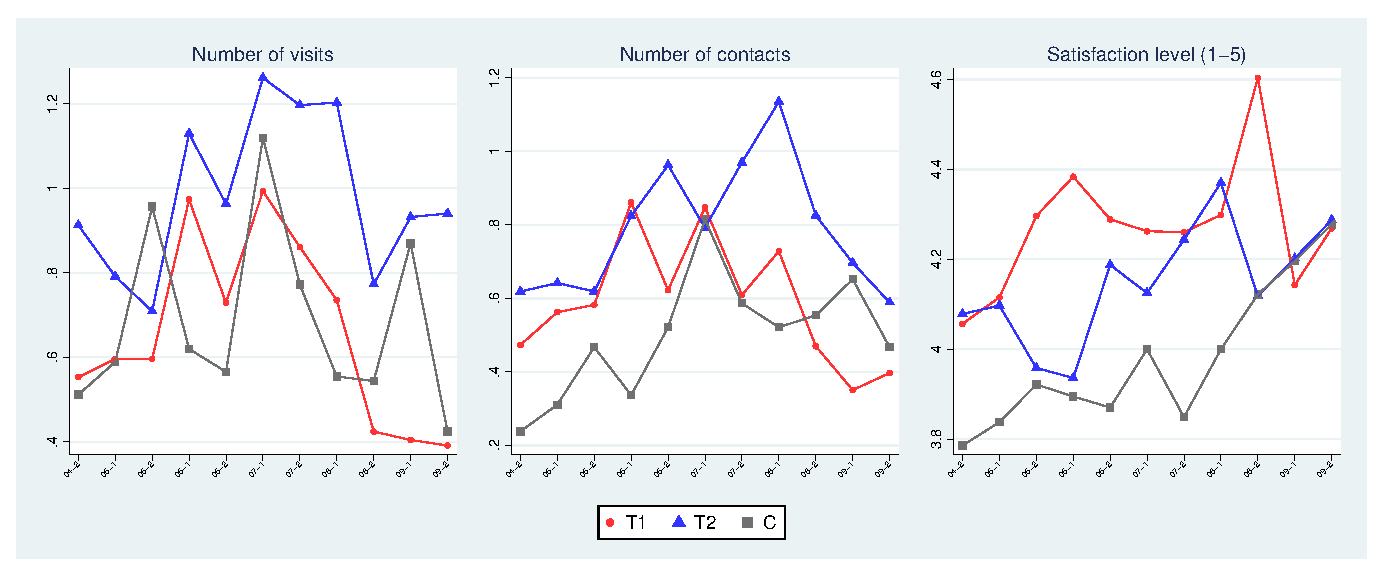
\includegraphics[width=12cm,height=0.78\textheight,keepaspectratio]{tmp/b_basic.eps}
	\end{figure}
\end{frame}

\begin{frame}{Satisfaction Level by District and Time}
	\begin{figure}
		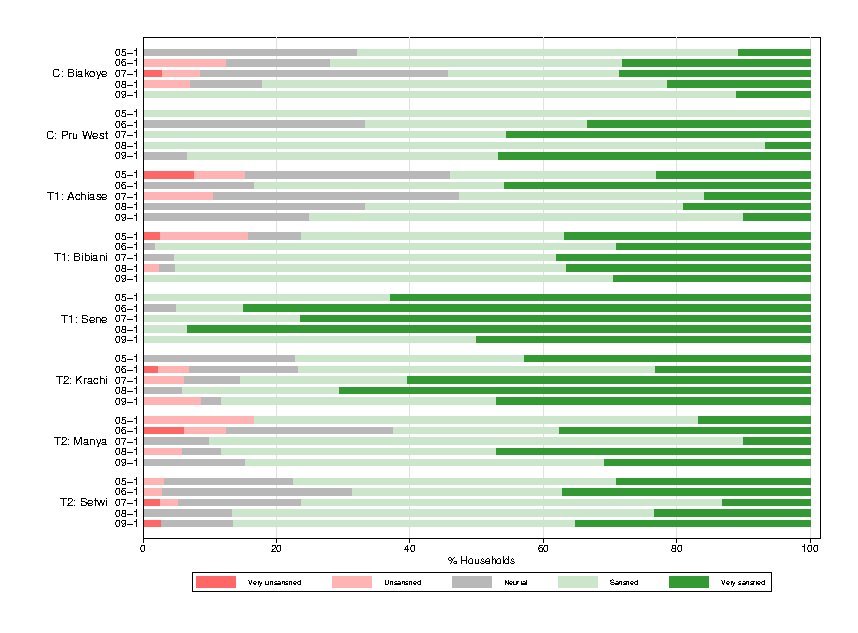
\includegraphics[width=10cm,height=0.78\textheight,keepaspectratio]{tmp/b_satisfy.eps}
	\end{figure}
\end{frame}

\begin{frame}{AEA Effort: Self-Reported vs Farmer-Reported Visits}
	\centering
	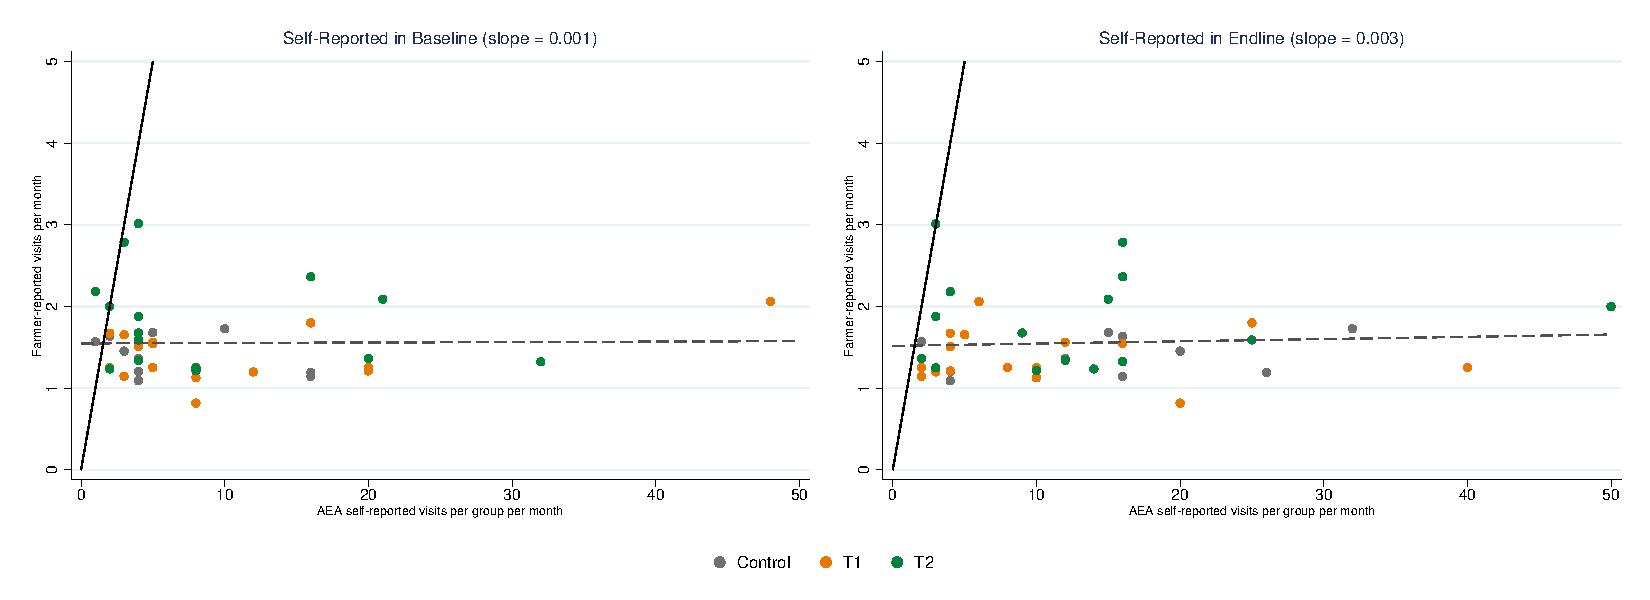
\includegraphics[width=\textwidth,keepaspectratio]{tmp/fig_selfrep_farmer.pdf}
	\begin{minipage}{0.94\textwidth}
		\notefont
		Note: one dot per AEA (N=41, rainfed sites only). Both axes are visits \emph{per month}. The AEA question asks
		``How often do you visit farmer group on average \ldots\ times per month'', so the
		self-report is already a per-group monthly rate and is used as answered; farmer reports are
		the mean cumulative visits over the 11 bi-weekly rounds divided by 5.5 months.
		Solid line: 45$^\circ$; dashed line and the slope in each panel title: OLS. All 41 AEAs
		are plotted.
		\par AEAs report 9.4 (baseline) and 13.0 (endline) visits per group per month against 1.6
		reported by farmers, and 42 of 43 lie below the 45$^\circ$ line.
		***, **, * : 1, 5, 10\%.
	\end{minipage}
\end{frame}

\begin{frame}{AEA Effort: Distance to the Communities Served}
	\centering
	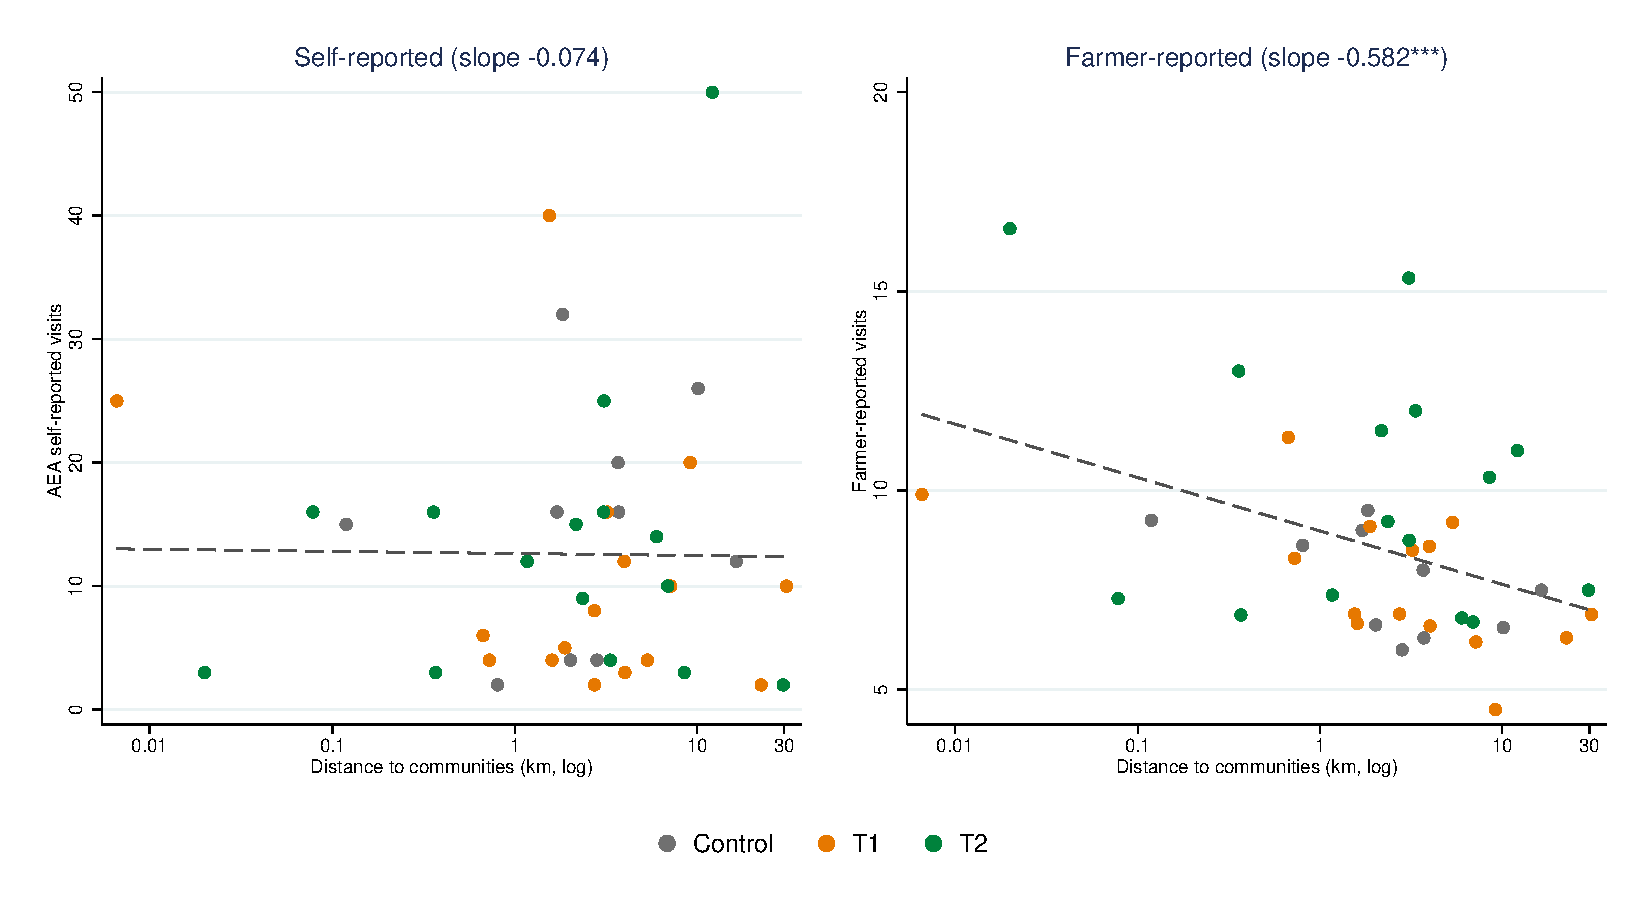
\includegraphics[width=\textwidth,keepaspectratio]{tmp/fig_dist_visits.pdf}
	\begin{minipage}{0.94\textwidth}
		\notefont
		Note: one dot per AEA (N=41, rainfed sites only; third panel: the AEAs with stamp records). Distance $=$
		mean distance from the AEA's duty station to the communities served, log scale. Dashed line
		and the slope in each panel title: OLS on $\ln$(distance). ***, **, * : 1, 5, 10\%.
	\end{minipage}
\end{frame}

\begin{frame}{Baseline -- Preliminary results of Correlation (AEA)}
	\centering
	\adjustbox{width=\textwidth,totalheight=0.70\textheight,keepaspectratio}{{
\def\sym#1{\ifmmode^{#1}\else\(^{#1}\)\fi}
\begin{tabular}{l*{5}{c}}
\hline\hline
                    &\multicolumn{1}{c}{(1)}         &\multicolumn{1}{c}{(2)}         &\multicolumn{1}{c}{(3)}         &\multicolumn{1}{c}{(4)}         &\multicolumn{1}{c}{(5)}         \\
                    &Prosocial         &Intrinsic         &Extrinsic         &Locus (Gen)         &Locus (Agri)         \\
\hline
Male (=1 yes)       &6.666\sym{**} &0.415         &-1.074         &-1.331         &-0.225         \\
                    &(2.588)         &(1.132)         &(2.074)         &(2.144)         &(1.744)         \\
Tenured (=1 yes)    &1.049         &-0.752         &0.046         &-0.575         &0.342         \\
                    &(0.767)         &(0.645)         &(0.765)         &(1.026)         &(1.122)         \\
G. Total years of experience as an extension agent:&0.037         &-0.067\sym{**} &0.061\sym{*}  &0.015         &-0.006         \\
                    &(0.038)         &(0.032)         &(0.033)         &(0.056)         &(0.079)         \\
K. Monthly salary (gross):&-0.000         &0.000         &-0.001\sym{*}  &0.000         &0.000         \\
                    &(0.000)         &(0.000)         &(0.000)         &(0.000)         &(0.000)         \\
E. Is motorbike provided by the office?&0.613         &-1.038         &0.238         &-0.982         &0.763         \\
                    &(0.928)         &(0.687)         &(0.686)         &(0.982)         &(1.137)         \\
Knowledge of Rice Production (0-4)&0.375         &-0.068         &0.266         &0.197         &-0.341         \\
                    &(0.307)         &(0.241)         &(0.305)         &(0.373)         &(0.483)         \\
Intrinsic motivation (2-10)&0.274         &              &0.435\sym{**} &-0.246         &0.406         \\
                    &(0.248)         &              &(0.174)         &(0.353)         &(0.309)         \\
Extrinsic motivation (2-10)&0.077         &0.380\sym{***}&              &0.008         &-0.275         \\
                    &(0.223)         &(0.121)         &              &(0.214)         &(0.242)         \\
General (F-J) (5-25)&0.193         &-0.098         &0.004         &              &0.486\sym{***}\\
                    &(0.211)         &(0.132)         &(0.098)         &              &(0.165)         \\
Agriculture (A-E) (5-25)&-0.072         &0.129         &-0.100         &0.389\sym{***}&              \\
                    &(0.133)         &(0.084)         &(0.084)         &(0.140)         &              \\
Total proscialness (6-30)&              &0.121         &0.039         &0.213         &-0.099         \\
                    &              &(0.122)         &(0.108)         &(0.249)         &(0.184)         \\
Constant            &13.798\sym{***}&3.343         &4.324         &8.547         &9.341\sym{*}  \\
                    &(3.794)         &(3.370)         &(3.854)         &(5.154)         &(5.452)         \\
\hline
Observations        &   42         &   42         &   42         &   42         &   42         \\
\hline\hline
\end{tabular}
}
}
	
\end{frame}

\begin{frame}{Endline -- Preliminary results of Correlation (AEA)}
	\centering
	\adjustbox{width=\textwidth,totalheight=0.70\textheight,keepaspectratio}{{
\def\sym#1{\ifmmode^{#1}\else\(^{#1}\)\fi}
\begin{tabular}{l*{5}{c}}
\hline\hline
                    &\multicolumn{1}{c}{(1)}         &\multicolumn{1}{c}{(2)}         &\multicolumn{1}{c}{(3)}         &\multicolumn{1}{c}{(4)}         &\multicolumn{1}{c}{(5)}         \\
                    &Prosocial         &Intrinsic         &Extrinsic         &Locus (Gen)         &Locus (Agri)         \\
\hline
Male (=1 yes)       &6.278         &2.273         &-0.795         &-3.443\sym{*}  &1.510         \\
                    &(5.059)         &(2.046)         &(2.180)         &(1.867)         &(1.914)         \\
F. Working tenure:  &-0.085         &0.652         &-0.768         &-1.347         &0.416         \\
                    &(0.946)         &(0.473)         &(0.537)         &(0.822)         &(0.850)         \\
G. Total years of experience as an extension agent:&0.050         &-0.075         &0.077         &0.113         &-0.113\sym{*}  \\
                    &(0.085)         &(0.056)         &(0.064)         &(0.078)         &(0.066)         \\
K. Monthly salary (gross):&0.000         &-0.000         &0.000         &-0.000         &0.001\sym{*}  \\
                    &(0.001)         &(0.000)         &(0.000)         &(0.000)         &(0.000)         \\
E. Is motorbike provided by the office?&-0.441         &-1.901\sym{**} &1.276         &2.308         &1.190         \\
                    &(2.079)         &(0.929)         &(1.096)         &(1.494)         &(1.319)         \\
Knowledge of rice production (0-5)&-0.534         &-0.382         &0.324         &-0.017         &0.713         \\
                    &(0.740)         &(0.369)         &(0.458)         &(0.654)         &(0.679)         \\
Intrinsic motivation (2-10)&-0.107         &              &0.384         &0.304         &0.503\sym{**} \\
                    &(0.432)         &              &(0.238)         &(0.273)         &(0.190)         \\
Extrinsic motivation (2-10)&-0.068         &0.228         &              &-0.284         &-0.266         \\
                    &(0.308)         &(0.161)         &              &(0.207)         &(0.182)         \\
Locus: general (5-25)&0.189         &0.114         &-0.180         &              &0.305\sym{*}  \\
                    &(0.273)         &(0.089)         &(0.139)         &              &(0.154)         \\
Locus: agriculture (5-25)&-0.113         &0.155\sym{*}  &-0.138         &0.249         &              \\
                    &(0.232)         &(0.083)         &(0.103)         &(0.169)         &              \\
Prosocialness (6-30)&              &-0.023         &-0.025         &0.107         &-0.079         \\
                    &              &(0.091)         &(0.113)         &(0.145)         &(0.173)         \\
Constant            &20.309\sym{**} &2.752         &6.901         &14.527\sym{***}&2.069         \\
                    &(9.000)         &(2.215)         &(4.896)         &(4.556)         &(4.346)         \\
\hline
Observations        &   41         &   41         &   41         &   41         &   41         \\
\hline\hline
\end{tabular}
}
}
	
\end{frame}

\begin{frame}{Baseline -- Preliminary results of Correlation (Farming)}
	\centering
	\adjustbox{width=\textwidth,totalheight=0.86\textheight,keepaspectratio}{{
\def\sym#1{\ifmmode^{#1}\else\(^{#1}\)\fi}
\begin{tabular}{l*{7}{c}}
\hline\hline
                    &\multicolumn{1}{c}{(1)}         &\multicolumn{1}{c}{(2)}         &\multicolumn{1}{c}{(3)}         &\multicolumn{1}{c}{(4)}         &\multicolumn{1}{c}{(5)}         &\multicolumn{1}{c}{(6)}         &\multicolumn{1}{c}{(7)}         \\
                    &Yield         &Log (Yield)         &Rice income (ha)         &Fertilizer (ha)         &Seed (ha)         &Hired labor(ha)         &Machinery (ha)         \\
\hline
Landsize (ha)       &-0.081         &-0.044         &-478.352         &-48.769         &-18.263         &-116.230         &175.963\sym{**} \\
                    &(0.043)         &(0.033)         &(364.775)         &(22.604)         &(8.438)         &(140.126)         &(46.212)         \\
Head age            &0.005         &-0.001         &-87.591         &0.725         &4.500\sym{**} &105.363         &0.048         \\
                    &(0.005)         &(0.003)         &(101.141)         &(3.986)         &(1.234)         &(99.095)         &(3.501)         \\
no edu              &0.000         &0.000         &0.000         &0.000         &0.000         &0.000         &0.000         \\
                    &  (.)         &  (.)         &  (.)         &  (.)         &  (.)         &  (.)         &  (.)         \\
primary             &-0.043         &-0.227         &1011.053         &352.887         &22.592         &-711.221         &-468.475\sym{*}  \\
                    &(0.339)         &(0.156)         &(2684.029)         &(313.572)         &(65.301)         &(1005.616)         &(187.642)         \\
junior high         &0.269         &-0.053         &1759.014         &100.063         &199.454         &-67.609         &25.525         \\
                    &(0.221)         &(0.148)         &(1962.700)         &(130.921)         &(96.396)         &(462.865)         &(64.729)         \\
senior high         &-0.225\sym{*}  &-0.253\sym{***}&-3.3e+03\sym{**} &34.660         &9.788         &1623.018\sym{**} &83.915         \\
                    &(0.087)         &(0.039)         &(869.052)         &(69.345)         &(87.159)         &(389.204)         &(42.394)         \\
tertiary            &-0.247         &-0.348         &-3.6e+03         &163.402         &-33.185         &1722.467         &23.131         \\
                    &(0.149)         &(0.148)         &(2554.623)         &(157.010)         &(65.267)         &(1982.255)         &(46.447)         \\
Head male (=1 yes)  &-0.489         &-0.283         &-6.6e+03         &-510.694         &158.284\sym{**} &2439.439\sym{**} &30.298         \\
                    &(0.414)         &(0.243)         &(3195.071)         &(314.556)         &(41.392)         &(473.499)         &(141.918)         \\
Fertilizer use (=1 yes)&0.267         &0.358         &533.570         &1512.300\sym{***}&-46.584         &44.563         &-22.365         \\
                    &(0.199)         &(0.163)         &(1553.037)         &(164.649)         &(39.512)         &(486.532)         &(59.891)         \\
Herbicides/Insecticides use (=1 yes)&-0.021         &0.048         &-727.982         &88.250         &-81.837         &315.920         &31.101         \\
                    &(0.248)         &(0.194)         &(1223.653)         &(124.799)         &(91.197)         &(1472.961)         &(67.768)         \\
Tractor (=1 yes)    &-0.437\sym{*}  &-0.370         &-3.6e+03         &177.367         &-159.693\sym{*}  &-1.1e+03         &805.405\sym{***}\\
                    &(0.147)         &(0.170)         &(2676.994)         &(197.646)         &(53.734)         &(1500.206)         &(140.887)         \\
Combine harvester (=1 yes)&1.657\sym{*}  &0.977\sym{**} &1.4e+04\sym{*}  &1072.299\sym{**} &216.034\sym{*}  &-2.1e+03         &1680.206\sym{**} \\
                    &(0.568)         &(0.214)         &(5010.995)         &(214.425)         &(71.582)         &(933.189)         &(452.270)         \\
Thresher (=1 yes)   &0.565\sym{***}&0.558\sym{***}&4471.094\sym{*}  &209.553         &-20.548         &-179.838         &466.781\sym{**} \\
                    &(0.099)         &(0.094)         &(1237.441)         &(151.406)         &(52.424)         &(820.341)         &(96.961)         \\
Other machinery (=1 yes)&1.079         &0.375         &8760.552         &317.994         &219.435         &631.921         &428.385\sym{*}  \\
                    &(0.562)         &(0.207)         &(6870.455)         &(258.390)         &(126.345)         &(1810.505)         &(152.214)         \\
Water/Salt treatment (=1 yes)&0.012         &0.087         &-1.9e+03         &305.662         &-104.978\sym{*}  &1120.631         &48.221         \\
                    &(0.177)         &(0.172)         &(1581.274)         &(275.381)         &(33.101)         &(1367.356)         &(81.765)         \\
CSIR-AGRA/Exbaika (=1 yes)&0.417\sym{**} &0.295\sym{*}  &-79.332         &-104.307         &5.824         &2368.900\sym{*}  &-101.528         \\
                    &(0.087)         &(0.096)         &(1244.638)         &(192.858)         &(110.391)         &(923.808)         &(88.922)         \\
Bunds construction (=1 yes)&0.356         &0.229         &274.393         &258.569         &156.300         &1776.762         &-214.394         \\
                    &(0.207)         &(0.103)         &(3008.358)         &(113.857)         &(104.138)         &(1801.680)         &(115.363)         \\
Levelling the field (=1 yes)&0.108         &-0.080         &-756.806         &102.658         &29.292         &1190.022         &-7.468         \\
                    &(0.262)         &(0.164)         &(1792.664)         &(93.096)         &(41.730)         &(845.768)         &(90.437)         \\
Any improved variety (=1 yes)&-0.372         &-0.241         &-1.6e+03         &299.298         &-19.236         &-1.5e+03\sym{*}  &233.285\sym{*}  \\
                    &(0.201)         &(0.161)         &(1896.887)         &(226.625)         &(109.548)         &(566.220)         &(96.507)         \\
Certified seed (=1 yes)&0.011         &0.075         &1060.866         &-94.177         &722.053\sym{***}&-943.025         &-50.387         \\
                    &(0.159)         &(0.186)         &(1269.710)         &(153.409)         &(88.997)         &(871.158)         &(68.733)         \\
Seed dibbling (=1 yes)&0.307         &0.492         &2068.006         &62.180         &-52.000         &1036.973         &48.755         \\
                    &(0.246)         &(0.313)         &(2518.148)         &(80.370)         &(29.085)         &(1116.319)         &(63.925)         \\
Transplanting in row (=1 yes)&1.266\sym{*}  &0.904\sym{*}  &9986.059         &17.659         &-202.337         &1775.599         &-181.887\sym{*}  \\
                    &(0.448)         &(0.260)         &(4703.609)         &(267.811)         &(144.339)         &(1061.121)         &(68.314)         \\
Constant            &1.420\sym{*}  &-0.122         &1.8e+04\sym{**} &92.969         &-48.451         &-4.8e+03         &-482.576\sym{**} \\
                    &(0.561)         &(0.480)         &(3535.671)         &(243.381)         &(152.252)         &(5418.600)         &(112.874)         \\
\hline
Obs                 &  354         &  354         &  321         &  378         &  378         &  378         &  378         \\
\hline\hline
\end{tabular}
}
}
	
\end{frame}

\begin{frame}{Endline -- Preliminary results of Correlation (Farming)}
	\centering
	\adjustbox{width=\textwidth,totalheight=0.86\textheight,keepaspectratio}{{
\def\sym#1{\ifmmode^{#1}\else\(^{#1}\)\fi}
\begin{tabular}{l*{9}{c}}
\hline\hline
                    &\multicolumn{1}{c}{(1)}         &\multicolumn{1}{c}{(2)}         &\multicolumn{1}{c}{(3)}         &\multicolumn{1}{c}{(4)}         &\multicolumn{1}{c}{(5)}         &\multicolumn{1}{c}{(6)}         &\multicolumn{1}{c}{(7)}         &\multicolumn{1}{c}{(8)}         &\multicolumn{1}{c}{(9)}         \\
                    &Yield         &Log (Yield)         &Revenue (ha)         &Income (ha)         &Profit (ha)         &Fertilizer (ha)         &Seed (ha)         &Hired labor(ha)         &Machinery (ha)         \\
\hline
Landsize (ha)       &-0.105         &-0.090\sym{**} &-645.964\sym{*}  &-373.017         &369.021         &-45.521         &82.244         &-169.701\sym{*}  &-52.056\sym{***}\\
                    &(0.055)         &(0.033)         &(329.594)         &(220.467)         &(358.872)         &(38.589)         &(119.969)         &(87.734)         &(6.620)         \\
Age of household head&0.006         &0.002         &17.138         &6.155         &-37.378         &-4.283         &-3.064         &16.291\sym{*}  &-3.884\sym{*}  \\
                    &(0.006)         &(0.004)         &(36.911)         &(33.510)         &(51.298)         &(4.224)         &(7.924)         &(7.783)         &(1.960)         \\
primary             &0.280         &0.171         &1638.727         &3331.208         &1866.539         &-307.727\sym{*}  &-548.746         &89.977         &67.436         \\
                    &(0.427)         &(0.206)         &(2645.490)         &(3108.356)         &(2031.122)         &(132.925)         &(638.520)         &(473.296)         &(135.770)         \\
junior high         &-0.026         &0.096         &-426.522         &1312.359         &-1.4e+03         &-102.824         &-145.754         &48.695         &-111.664         \\
                    &(0.385)         &(0.258)         &(2382.564)         &(1462.619)         &(2536.818)         &(193.238)         &(302.509)         &(553.543)         &(122.000)         \\
senior high         &-0.228         &-0.062         &-2.2e+03\sym{*}  &-614.430         &-1.5e+03         &-377.311\sym{*}  &-176.217         &-365.845         &-0.812         \\
                    &(0.195)         &(0.136)         &(1135.646)         &(641.634)         &(2212.884)         &(184.233)         &(95.429)         &(326.933)         &(27.743)         \\
tertiary            &0.074         &0.083         &-114.583         &437.758         &474.404         &-174.850         &172.756         &37.742         &109.482\sym{***}\\
                    &(0.084)         &(0.070)         &(655.450)         &(881.216)         &(1404.555)         &(209.619)         &(237.555)         &(433.018)         &(22.824)         \\
Gender of household head&0.026         &-0.018         &810.490         &-30.650         &1879.912         &-243.853         &595.446         &165.881         &14.940         \\
                    &(0.461)         &(0.223)         &(2720.908)         &(2340.357)         &(3384.048)         &(382.819)         &(578.759)         &(457.403)         &(131.739)         \\
Chemical fertilizer (=1 yes)&0.328\sym{**} &0.232\sym{**} &2150.218\sym{**} &-134.754         &-1.3e+03         &1393.264\sym{***}&54.551         &726.782\sym{**} &-16.029         \\
                    &(0.132)         &(0.072)         &(777.964)         &(887.373)         &(1299.511)         &(112.815)         &(79.780)         &(268.092)         &(33.443)         \\
Herbicide/insecticide (=1 yes)&0.264         &0.068         &1542.970\sym{*}  &427.003         &-3.7e+03\sym{*}  &58.943         &79.565         &29.119         &-50.312         \\
                    &(0.141)         &(0.097)         &(805.228)         &(499.601)         &(1590.788)         &(174.638)         &(79.020)         &(163.347)         &(37.060)         \\
Tractor (=1 yes)    &-0.401\sym{**} &-0.343\sym{*}  &-2.8e+03\sym{**} &-2.5e+03\sym{**} &2288.804\sym{*}  &-169.663         &-83.879         &-444.657         &920.307\sym{***}\\
                    &(0.159)         &(0.153)         &(984.321)         &(768.710)         &(1099.508)         &(196.787)         &(100.528)         &(385.319)         &(98.712)         \\
Combine harvester (=1 yes)&2.215\sym{***}&1.053\sym{***}&1.3e+04\sym{***}&6360.589\sym{***}&6756.211\sym{*}  &1161.893\sym{***}&2138.397         &99.535         &2158.089\sym{***}\\
                    &(0.288)         &(0.126)         &(1978.721)         &(1494.548)         &(2934.540)         &(294.666)         &(1302.954)         &(568.856)         &(239.112)         \\
Thresher (=1 yes)   &0.286         &0.152         &2322.998         &1946.783         &2779.194         &178.303         &-3.777         &4.551         &564.712\sym{***}\\
                    &(0.229)         &(0.133)         &(1262.477)         &(1287.319)         &(1838.056)         &(318.920)         &(103.109)         &(291.089)         &(65.636)         \\
Other machinery (=1 yes)&-1.492         &-0.749         &-8.5e+03         &-9.3e+03\sym{**} &-9.0e+03\sym{**} &266.434         &-1.3e+03         &90.706         &2104.934         \\
                    &(1.034)         &(0.713)         &(6119.260)         &(3343.955)         &(3202.404)         &(345.069)         &(1589.992)         &(571.144)         &(1772.011)         \\
Seed treatment (=1 yes)&-0.180         &-0.143         &-1.6e+03         &-1.3e+03         &-6.0e+03\sym{***}&21.144         &-209.467         &-181.316         &24.553         \\
                    &(0.208)         &(0.117)         &(1320.400)         &(985.929)         &(1318.913)         &(103.212)         &(222.098)         &(361.425)         &(86.079)         \\
Improved seed (=1 yes)&0.121         &-0.127         &34.445         &-96.418         &-2.9e+03         &644.914         &231.801         &-385.824         &18.750         \\
                    &(0.470)         &(0.300)         &(2501.572)         &(1711.579)         &(2193.722)         &(354.818)         &(370.718)         &(498.217)         &(159.878)         \\
Bunds construction (=1 yes)&0.259         &0.249\sym{**} &1742.362         &296.130         &1047.161         &121.786         &1014.695         &540.098         &75.911         \\
                    &(0.186)         &(0.095)         &(1253.751)         &(1007.397)         &(1725.692)         &(109.149)         &(961.920)         &(609.663)         &(66.298)         \\
Levelling the field (=1 yes)&0.023         &0.022         &62.378         &957.999         &1292.091         &147.092         &-725.378         &199.452         &-46.617         \\
                    &(0.133)         &(0.102)         &(812.654)         &(1268.466)         &(1332.076)         &(150.166)         &(722.029)         &(227.437)         &(35.752)         \\
Any improved variety (=1 yes)&0.142         &0.204         &817.320         &767.895         &-121.645         &-21.681         &-270.057         &322.000         &34.183         \\
                    &(0.155)         &(0.149)         &(1004.533)         &(835.441)         &(1209.630)         &(149.261)         &(213.771)         &(414.134)         &(77.662)         \\
Certified seed (=1 yes)&0.486\sym{**} &0.130\sym{*}  &3339.313\sym{**} &1621.409         &5930.265\sym{**} &156.018         &1283.479\sym{*}  &295.008         &44.470         \\
                    &(0.180)         &(0.062)         &(1087.369)         &(1086.060)         &(2290.950)         &(152.486)         &(669.729)         &(292.913)         &(76.025)         \\
Seed dibbling (=1 yes)&0.214         &0.176         &1833.690\sym{**} &1022.227         &887.714         &-34.961         &-26.742         &525.754         &-22.209         \\
                    &(0.115)         &(0.108)         &(765.765)         &(715.341)         &(1726.913)         &(126.387)         &(113.386)         &(300.172)         &(70.201)         \\
Transplanting in row (=1 yes)&0.493\sym{*}  &0.223         &2976.106\sym{**} &1241.163         &-4.5e+03         &140.439         &-431.916         &1250.512\sym{*}  &-24.317         \\
                    &(0.231)         &(0.143)         &(1076.110)         &(1532.139)         &(5630.335)         &(196.813)         &(910.933)         &(546.112)         &(128.662)         \\
Constant            &0.769         &-0.178         &5273.296         &2823.020         &-1.5e+03         &554.232         &-175.228         &1081.670         &251.550\sym{*}  \\
                    &(0.734)         &(0.401)         &(4333.594)         &(3279.816)         &(3051.320)         &(590.172)         &(202.877)         &(865.551)         &(126.310)         \\
\hline
Obs                 &  382         &  370         &  382         &  382         &  382         &  382         &  382         &  382         &  382         \\
\hline\hline
\end{tabular}
}
}
	
\end{frame}

\begin{frame}{Baseline -- Correlates of Practice Adoption (Farming)}
	\centering
	\adjustbox{width=\textwidth,totalheight=0.70\textheight,keepaspectratio}{{
\def\sym#1{\ifmmode^{#1}\else\(^{#1}\)\fi}
\begin{tabular}{l*{8}{c}}
\hline\hline
                    &\multicolumn{1}{c}{(1)}         &\multicolumn{1}{c}{(2)}         &\multicolumn{1}{c}{(3)}         &\multicolumn{1}{c}{(4)}         &\multicolumn{1}{c}{(5)}         &\multicolumn{1}{c}{(6)}         &\multicolumn{1}{c}{(7)}         &\multicolumn{1}{c}{(8)}         \\
                    &Any improved         &Certified         &Seed trt         &Dibbling         &Row trans         &Bunds         &Levelling         &No. practices         \\
\hline
Landsize (ha)       &-0.056\sym{***}&-0.010         &-0.017\sym{***}&-0.042\sym{**} &-0.007         &-0.012         &0.022\sym{**} &-0.121\sym{***}\\
                    &(0.006)         &(0.010)         &(0.004)         &(0.014)         &(0.004)         &(0.007)         &(0.008)         &(0.024)         \\
Age of household head&0.004         &0.002         &0.002\sym{*}  &0.001         &-0.000         &-0.000         &0.001         &0.009         \\
                    &(0.003)         &(0.001)         &(0.001)         &(0.002)         &(0.001)         &(0.002)         &(0.002)         &(0.006)         \\
primary             &0.335\sym{*}  &0.221         &0.055         &0.027         &-0.015         &0.114         &0.137         &0.875\sym{**} \\
                    &(0.142)         &(0.161)         &(0.103)         &(0.173)         &(0.018)         &(0.077)         &(0.113)         &(0.294)         \\
junior high         &0.054         &0.116         &0.118         &-0.106         &0.027         &0.035         &0.125         &0.368         \\
                    &(0.066)         &(0.116)         &(0.077)         &(0.088)         &(0.034)         &(0.063)         &(0.085)         &(0.205)         \\
senior high         &0.081         &0.082         &0.075\sym{*}  &-0.017         &0.028         &0.037         &0.053         &0.339\sym{**} \\
                    &(0.105)         &(0.063)         &(0.034)         &(0.098)         &(0.023)         &(0.027)         &(0.041)         &(0.137)         \\
tertiary            &0.092         &0.082         &0.039         &-0.249\sym{**} &0.043\sym{*}  &0.076         &0.088         &0.171         \\
                    &(0.078)         &(0.054)         &(0.046)         &(0.077)         &(0.021)         &(0.061)         &(0.055)         &(0.134)         \\
Gender of household head&0.026         &-0.101         &0.080         &0.156         &-0.069         &-0.049         &-0.102         &-0.059         \\
                    &(0.092)         &(0.136)         &(0.101)         &(0.113)         &(0.047)         &(0.116)         &(0.169)         &(0.539)         \\
Household size      &-0.021\sym{***}&-0.004         &-0.005         &-0.006         &-0.006\sym{*}  &-0.013         &0.007         &-0.050\sym{*}  \\
                    &(0.003)         &(0.004)         &(0.005)         &(0.011)         &(0.003)         &(0.007)         &(0.007)         &(0.022)         \\
Total assets owned  &0.000         &-0.000         &0.000         &-0.000         &0.000         &-0.000         &0.000         &0.000         \\
                    &(0.000)         &(0.000)         &(0.000)         &(0.000)         &(0.000)         &(0.000)         &(0.000)         &(0.000)         \\
Constant            &0.610\sym{**} &0.206         &-0.033         &0.353         &0.152\sym{*}  &0.252         &0.137         &1.677\sym{**} \\
                    &(0.208)         &(0.158)         &(0.100)         &(0.217)         &(0.077)         &(0.166)         &(0.231)         &(0.686)         \\
\hline
Obs                 &  378         &  378         &  378         &  378         &  378         &  378         &  378         &  378         \\
\hline\hline
\end{tabular}
}
}
	\begin{minipage}{0.94\textwidth}
		\notefont
		Note: OLS at baseline; each column regresses the practice indicator (No.\ practices
		$=$ count of the seven) on household characteristics; SE clustered at district.
		***, **, * : 1, 5, 10\%.
	\end{minipage}
\end{frame}

\begin{frame}{Endline -- Correlates of Practice Adoption (Farming)}
	\centering
	\adjustbox{width=\textwidth,totalheight=0.70\textheight,keepaspectratio}{{
\def\sym#1{\ifmmode^{#1}\else\(^{#1}\)\fi}
\begin{tabular}{l*{8}{c}}
\hline\hline
                    &\multicolumn{1}{c}{(1)}         &\multicolumn{1}{c}{(2)}         &\multicolumn{1}{c}{(3)}         &\multicolumn{1}{c}{(4)}         &\multicolumn{1}{c}{(5)}         &\multicolumn{1}{c}{(6)}         &\multicolumn{1}{c}{(7)}         &\multicolumn{1}{c}{(8)}         \\
                    &Any improved         &Certified         &Seed trt         &Dibbling         &Row trans         &Bunds         &Levelling         &No. practices         \\
\hline
Landsize (ha)       &-0.039\sym{**} &-0.008         &-0.008         &-0.027\sym{*}  &-0.001         &-0.007         &0.040\sym{***}&-0.050\sym{**} \\
                    &(0.013)         &(0.009)         &(0.007)         &(0.012)         &(0.007)         &(0.005)         &(0.009)         &(0.020)         \\
Age of household head&0.002         &-0.000         &0.004         &-0.000         &0.000         &-0.002         &-0.000         &0.004         \\
                    &(0.003)         &(0.002)         &(0.003)         &(0.003)         &(0.001)         &(0.002)         &(0.003)         &(0.009)         \\
primary             &-0.024         &0.165         &0.020         &0.164         &-0.025         &0.063         &-0.064         &0.299         \\
                    &(0.156)         &(0.166)         &(0.106)         &(0.163)         &(0.019)         &(0.124)         &(0.151)         &(0.257)         \\
junior high         &0.016         &0.090\sym{*}  &0.232\sym{**} &0.071         &0.055         &-0.063         &-0.072         &0.329         \\
                    &(0.062)         &(0.040)         &(0.080)         &(0.117)         &(0.035)         &(0.048)         &(0.077)         &(0.239)         \\
senior high         &0.049         &0.110\sym{**} &0.136\sym{*}  &0.029         &0.061\sym{***}&-0.038         &-0.061         &0.286\sym{*}  \\
                    &(0.082)         &(0.038)         &(0.058)         &(0.093)         &(0.014)         &(0.058)         &(0.083)         &(0.136)         \\
tertiary            &-0.037         &0.101\sym{**} &0.074         &-0.089         &0.023         &0.017         &-0.053         &0.035         \\
                    &(0.070)         &(0.040)         &(0.083)         &(0.053)         &(0.029)         &(0.060)         &(0.064)         &(0.157)         \\
Gender of household head&0.068         &-0.042         &0.027         &0.160         &-0.025         &-0.353\sym{**} &-0.282\sym{**} &-0.447         \\
                    &(0.095)         &(0.080)         &(0.118)         &(0.090)         &(0.066)         &(0.114)         &(0.108)         &(0.278)         \\
Household size      &-0.012         &-0.012\sym{*}  &-0.006         &-0.000         &-0.007\sym{**} &0.003         &-0.000         &-0.034\sym{*}  \\
                    &(0.010)         &(0.006)         &(0.009)         &(0.013)         &(0.003)         &(0.008)         &(0.013)         &(0.018)         \\
Total assets owned  &-0.000\sym{*}  &0.000         &0.000\sym{**} &0.000         &0.000         &0.000         &0.000\sym{*}  &0.000         \\
                    &(0.000)         &(0.000)         &(0.000)         &(0.000)         &(0.000)         &(0.000)         &(0.000)         &(0.000)         \\
Constant            &0.647\sym{**} &0.226         &-0.012         &0.190         &0.077         &0.545\sym{**} &0.587\sym{**} &2.261\sym{***}\\
                    &(0.227)         &(0.160)         &(0.195)         &(0.197)         &(0.132)         &(0.189)         &(0.219)         &(0.526)         \\
\hline
Obs                 &  382         &  382         &  382         &  382         &  382         &  382         &  382         &  382         \\
\hline\hline
\end{tabular}
}
}
	\begin{minipage}{0.94\textwidth}
		\notefont
		Note: OLS at endline; each column regresses the practice indicator (No.\ practices
		$=$ count of the seven) on household characteristics; SE clustered at district.
		***, **, * : 1, 5, 10\%.
		\par Levelling rises with plot size alongside mechanisation: in the smallest area quartile
		(mean 0.63\,ha) 31.3\% level and 38.1\% use any machine (27.6\% a tractor), against 48.3\%
		and 65.2\% (58.4\% a tractor) in the largest quartile (mean 4.42\,ha). Bunds move the other
		way (18.7\% in Q1 vs 12.4\% in Q4), so the negative area gradient in the table is on bunds,
		not levelling.
	\end{minipage}
\end{frame}









% ======================= ENDLINE IMPACT RESULTS =======================






\begin{frame}{Empirical Strategy}
\begin{itemize}
	\item \textbf{ANCOVA}: regress endline outcome on treatment status, controlling for
	      the baseline value of the outcome
	\item Arms: T1 (Feedback), T2 (Feedback + Training); plus the cross-cutting Stamp (GPS)
	\item \textbf{Sample}: \emph{rainfed sites only} --- the two irrigation schemes (Kpong and
	      Weta) are dropped from every estimation (12 farmers, 2 AEAs, all in the control arm;
	      yields, seed rates and labour there are on a different scale). Farmers $N=382$, AEAs $N=41$
	\item Farmer models add region (province) FE; SEs clustered at district
	      (\textbf{8 clusters}: 2 control, 3 T1, 3 T2)
	\item Few clusters $\Rightarrow$ \textbf{wild cluster bootstrap} (Webb, 9{,}999) and
	      \textbf{randomization-inference} $p$-values alongside clustered SEs. With 2 control
	      districts these bind --- read the clustered SEs as the optimistic bound
	\item Crop failure = realized \textbf{zero} output (kept in sample); logs use $\ln(1+x)$;
	      outcomes are not winsorized
\end{itemize}
\end{frame}

\begin{frame}{AEA: Motivation and Locus of Control}
	\centering
	\adjustbox{width=\textwidth,totalheight=0.70\textheight,keepaspectratio}{{
\def\sym#1{\ifmmode^{#1}\else\(^{#1}\)\fi}
\begin{tabular}{l*{5}{c}}
\toprule
                    &\multicolumn{1}{c}{(1)}&\multicolumn{1}{c}{(2)}&\multicolumn{1}{c}{(3)}&\multicolumn{1}{c}{(4)}&\multicolumn{1}{c}{(5)}\\
                    &\multicolumn{1}{c}{Intrinsic}&\multicolumn{1}{c}{Extrinsic}&\multicolumn{1}{c}{Prosocial}&\multicolumn{1}{c}{Locus: gen}&\multicolumn{1}{c}{Locus: agri}\\
\midrule
T1: Feedback        &      -0.578         &       0.249         &       0.510         &       2.133\sym{***}&       2.709         \\
                    &     (1.087)         &     (0.269)         &     (1.090)         &     (0.412)         &     (1.576)         \\
T2: Feedback+Training&      -0.568         &      -0.317         &      -0.271         &      -0.234         &       3.129\sym{***}\\
                    &     (0.468)         &     (0.317)         &     (0.817)         &     (0.629)         &     (0.853)         \\
Stamp (GPS)         &      -0.131         &       0.124         &       0.134         &       1.746         &      -0.613         \\
                    &     (0.423)         &     (0.702)         &     (0.632)         &     (1.175)         &     (1.618)         \\
\midrule
T1=T2 [p]           &       0.992         &       0.138         &       0.371         &       0.008         &       0.780         \\
Ctrl mean (base)    &       6.500         &       5.000         &      26.900         &      18.300         &      17.300         \\
Ctrl mean (end)     &       7.000         &       5.000         &      25.900         &      18.800         &      13.900         \\
Wild-boot p (T1)    &       0.678         &       0.493         &       0.770         &       0.025         &       0.130         \\
Wild-boot p (T2)    &       0.509         &       0.301         &       0.770         &       0.667         &       0.034         \\
RI p (T1)           &       0.636         &       0.369         &       0.656         &       0.000         &       0.145         \\
RI p (T2)           &       0.310         &       0.364         &       0.766         &       0.750         &       0.022         \\
Obs                 &          41         &          41         &          41         &          41         &          41         \\
\bottomrule
\end{tabular}
}
}
	\begin{minipage}{0.94\textwidth}
		\notefont
		Note: ANCOVA controlling for the baseline value; SE clustered at district ($N=41$ AEAs, 8 districts).
		Wild-boot = Webb wild cluster bootstrap (9{,}999); RI = randomization inference (1{,}000).
		***, **, * : 1, 5, 10\%.
	\end{minipage}
\end{frame}

\begin{frame}{AEA: Knowledge, Effort, Satisfaction}
	\centering
	\adjustbox{width=\textwidth,totalheight=0.52\textheight,keepaspectratio}{{
\def\sym#1{\ifmmode^{#1}\else\(^{#1}\)\fi}
\begin{tabular}{l*{6}{c}}
\toprule
                    &\multicolumn{1}{c}{(1)}&\multicolumn{1}{c}{(2)}&\multicolumn{1}{c}{(3)}&\multicolumn{1}{c}{(4)}&\multicolumn{1}{c}{(5)}&\multicolumn{1}{c}{(6)}\\
                    &\multicolumn{1}{c}{Knowledge (0--5)}&\multicolumn{1}{c}{Knowledge (0--8)}&\multicolumn{1}{c}{Training attend.}&\multicolumn{1}{c}{Knowl. (0--5) direct}&\multicolumn{1}{c}{Self-rep. visits}&\multicolumn{1}{c}{Job satisf.}\\
\midrule
T1: Feedback        &       0.472\sym{**} &       0.919\sym{**} &      -0.020         &       0.487\sym{**} &      -4.327         &      -0.053         \\
                    &     (0.196)         &     (0.306)         &     (0.076)         &     (0.159)         &     (2.687)         &     (0.718)         \\
T2: Feedback+Training&       0.923\sym{**} &       1.498\sym{*}  &       0.074\sym{*}  &       0.875\sym{**} &      -1.668\sym{**} &       0.143         \\
                    &     (0.292)         &     (0.718)         &     (0.036)         &     (0.292)         &     (0.631)         &     (0.589)         \\
Attended training (=1)&                     &                     &                     &       0.497\sym{**} &                     &                     \\
                    &                     &                     &                     &     (0.171)         &                     &                     \\
Stamp (GPS)         &      -0.686         &      -1.297\sym{**} &       0.042         &      -0.705         &      -1.805         &      -0.218         \\
                    &     (0.416)         &     (0.486)         &     (0.039)         &     (0.416)         &     (5.428)         &     (0.243)         \\
\midrule
T1=T2 [p]           &       0.159         &       0.316         &       0.148         &       0.206         &       0.336         &       0.714         \\
Ctrl mean (base)    &       2.300         &       3.100         &       0.500         &       2.300         &       6.500         &       3.500         \\
Ctrl mean (end)     &       2.300         &       3.800         &       0.900         &       2.300         &      14.700         &       3.900         \\
Wild-boot p (T1)    &       0.053         &       0.064         &       0.831         &       0.037         &       0.276         &       0.957         \\
Wild-boot p (T2)    &       0.066         &       0.145         &       0.115         &       0.092         &       0.121         &       0.740         \\
RI p (T1)           &       0.066         &       0.022         &       0.818         &       0.022         &       0.191         &       0.952         \\
RI p (T2)           &       0.024         &       0.111         &       0.065         &       0.023         &       0.034         &       0.818         \\
Obs                 &          41         &          41         &          41         &          41         &          41         &          41         \\
\bottomrule
\end{tabular}
}
}
	\begin{minipage}{0.94\textwidth}
		\notefont
		Note: ANCOVA controlling for the baseline value; SE clustered at district ($N=41$, 8 districts).
		Knowledge (0--8) replaces the earlier 0--5 index: item A (``seed selection by salt or urea
		water is good for what?'') is a \emph{multiple}-response question and the old 0/1 coding
		scored 1 for every AEA in both waves, so it carried no information; the new score counts how
		many of the four defensible purposes are named and adds the four single-choice items.
		Self-reported visits remain noisy --- the bi-weekly farmer reports are the preferred effort
		measure.
		\par \textbf{Mediation analysis:} The indirect share is $-3.2\%$ (T1) and $5.2\%$ (T2). 
		Restricting the mediator to
		JICA-provided courses gives the same picture ($-2.3\%$ and $1.9\%$).
		\emph{Caveat}: a post-treatment mediator is a bad control, so this split is descriptive,
		not a causal mediation estimate.
		***, **, * : 1, 5, 10\%.
	\end{minipage}
\end{frame}

\begin{frame}{Bi-weekly (AEA): Effort Level Reported by Farmers}
	\centering
	\adjustbox{width=\textwidth,totalheight=0.66\textheight,keepaspectratio}{{
\def\sym#1{\ifmmode^{#1}\else\(^{#1}\)\fi}
\begin{tabular}{l*{6}{c}}
\toprule
                    &\multicolumn{2}{c}{All rounds (Apr--Sep)}  &\multicolumn{2}{c}{Planting window (05-1--06-2)}&\multicolumn{2}{c}{Growing season (07-1--08-2)}\\\cmidrule(lr){2-3}\cmidrule(lr){4-5}\cmidrule(lr){6-7}
                    &\multicolumn{1}{c}{(1)}&\multicolumn{1}{c}{(2)}&\multicolumn{1}{c}{(3)}&\multicolumn{1}{c}{(4)}&\multicolumn{1}{c}{(5)}&\multicolumn{1}{c}{(6)}\\
                    &\multicolumn{1}{c}{Visits}&\multicolumn{1}{c}{Contacts}&\multicolumn{1}{c}{Visits}&\multicolumn{1}{c}{Contacts}&\multicolumn{1}{c}{Visits}&\multicolumn{1}{c}{Contacts}\\
\midrule
T1: Feedback        &      -0.043         &      -0.057         &       0.111         &       0.146\sym{**} &      -0.060         &      -0.169         \\
                    &     (0.059)         &     (0.075)         &     (0.146)         &     (0.052)         &     (0.117)         &     (0.163)         \\
T2: Feedback+Training&       0.150\sym{**} &       0.057         &       0.140         &       0.159\sym{***}&       0.164         &       0.048         \\
                    &     (0.050)         &     (0.057)         &     (0.133)         &     (0.042)         &     (0.089)         &     (0.120)         \\
Stamp (GPS)         &       0.121         &       0.046         &       0.185         &      -0.019         &       0.132         &       0.078         \\
                    &     (0.114)         &     (0.186)         &     (0.106)         &     (0.201)         &     (0.187)         &     (0.272)         \\
\midrule
T1=T2 [p]           &       0.027         &       0.387         &       0.729         &       0.867         &       0.272         &       0.460         \\
Control mean        &       0.511         &       0.239         &       0.683         &       0.410         &       0.747         &       0.620         \\
Wild-boot p (T1)    &       0.709         &       0.707         &       0.869         &       0.243         &       0.769         &       0.547         \\
Wild-boot p (T2)    &       0.187         &       0.548         &       0.700         &       0.166         &       0.369         &       0.807         \\
RI p (T1)           &       0.486         &       0.492         &       0.481         &       0.021         &       0.626         &       0.339         \\
RI p (T2)           &       0.022         &       0.365         &       0.320         &       0.004         &       0.087         &       0.705         \\
Obs                 &        4120         &        4120         &        1503         &        1503         &        1499         &        1499         \\
\bottomrule
\end{tabular}
}
}
	\begin{minipage}{0.94\textwidth}
		\notefont
		Note: farmer$\times$round panel, estimated by OLS; outcomes are the \emph{number} of AEA
		visits and contacts the farmer reports in the two-week round. Three seasonal windows: all 11 rounds, the
		planting/establishment window (05-1--06-2) and the growing/harvest window (07-1--09-2).
		Round and province FE; SE clustered at district. Control mean measured in the first round
		(all-rounds columns) or within the window. Wild-boot (Webb, 9{,}999) and RI (1{,}000)
		$p$-values. ***, **, * : 1, 5, 10\%.
	\end{minipage}
\end{frame}

\begin{frame}{Bi-weekly (farmer): Satisfaction to Extension Service}
	\centering
	\adjustbox{width=\textwidth,totalheight=0.66\textheight,keepaspectratio}{{
\def\sym#1{\ifmmode^{#1}\else\(^{#1}\)\fi}
\begin{tabular}{l*{12}{c}}
\toprule
                    &\multicolumn{4}{c}{All rounds (Apr--Sep)}                                              &\multicolumn{4}{c}{Planting window (05-1--06-2)}                                       &\multicolumn{4}{c}{Growing season (07-1--08-2)}                                        \\\cmidrule(lr){2-5}\cmidrule(lr){6-9}\cmidrule(lr){10-13}
                    &\multicolumn{1}{c}{(1)}&\multicolumn{1}{c}{(2)}&\multicolumn{1}{c}{(3)}&\multicolumn{1}{c}{(4)}&\multicolumn{1}{c}{(5)}&\multicolumn{1}{c}{(6)}&\multicolumn{1}{c}{(7)}&\multicolumn{1}{c}{(8)}&\multicolumn{1}{c}{(9)}&\multicolumn{1}{c}{(10)}&\multicolumn{1}{c}{(11)}&\multicolumn{1}{c}{(12)}\\
                    &\multicolumn{1}{c}{Satisfied}&\multicolumn{1}{c}{Satisfied (full)}&\multicolumn{1}{c}{Add.\ ctrl}&\multicolumn{1}{c}{Full, add.\ ctrl}&\multicolumn{1}{c}{Satisfied}&\multicolumn{1}{c}{Satisfied (full)}&\multicolumn{1}{c}{Add.\ ctrl}&\multicolumn{1}{c}{Full, add.\ ctrl}&\multicolumn{1}{c}{Satisfied}&\multicolumn{1}{c}{Satisfied (full)}&\multicolumn{1}{c}{Add.\ ctrl}&\multicolumn{1}{c}{Full, add.\ ctrl}\\
\midrule
T1: Feedback        &       0.147\sym{**} &       0.055\sym{*}  &       0.152\sym{**} &       0.069\sym{**} &       0.161\sym{**} &       0.214\sym{***}&       0.167\sym{**} &       0.173\sym{***}&       0.151\sym{*}  &       0.022         &       0.154\sym{*}  &       0.041         \\
                    &     (0.047)         &     (0.027)         &     (0.047)         &     (0.026)         &     (0.048)         &     (0.047)         &     (0.057)         &     (0.011)         &     (0.073)         &     (0.077)         &     (0.067)         &     (0.051)         \\
T2: Feedback+Training&       0.075\sym{**} &       0.043\sym{*}  &       0.062\sym{**} &       0.001         &       0.044         &       0.093\sym{*}  &       0.034         &       0.043\sym{**} &       0.124\sym{**} &       0.046         &       0.112\sym{**} &       0.005         \\
                    &     (0.025)         &     (0.020)         &     (0.026)         &     (0.025)         &     (0.032)         &     (0.042)         &     (0.039)         &     (0.015)         &     (0.038)         &     (0.064)         &     (0.034)         &     (0.046)         \\
Stamp (GPS)         &       0.049         &       0.051         &       0.043         &       0.018         &       0.042         &       0.074         &       0.028         &       0.019         &       0.054         &       0.079         &       0.051         &       0.045         \\
                    &     (0.030)         &     (0.055)         &     (0.027)         &     (0.033)         &     (0.032)         &     (0.043)         &     (0.029)         &     (0.026)         &     (0.037)         &     (0.086)         &     (0.034)         &     (0.046)         \\
Number visits (2 weeks)&                     &                     &       0.062\sym{**} &       0.259\sym{***}&                     &                     &       0.100\sym{**} &       0.304\sym{***}&                     &                     &       0.054\sym{**} &       0.238\sym{***}\\
                    &                     &                     &     (0.018)         &     (0.033)         &                     &                     &     (0.030)         &     (0.037)         &                     &                     &     (0.022)         &     (0.052)         \\
Number contacts (2 weeks)&                     &                     &       0.006         &       0.048         &                     &                     &       0.010         &       0.051         &                     &                     &       0.004         &       0.028         \\
                    &                     &                     &     (0.005)         &     (0.025)         &                     &                     &     (0.012)         &     (0.033)         &                     &                     &     (0.004)         &     (0.020)         \\
\midrule
T1=T2 [p]           &       0.230         &       0.792         &       0.121         &       0.042         &       0.034         &       0.011         &       0.025         &       0.001         &       0.776         &       0.817         &       0.628         &       0.524         \\
Control mean        &       0.750         &       0.239         &       0.750         &       0.239         &       0.750         &       0.369         &       0.750         &       0.369         &       0.794         &       0.418         &       0.794         &       0.418         \\
Wild-boot p (T1)    &       0.203         &       0.272         &       0.189         &       0.185         &       0.238         &       0.112         &       0.250         &       0.040         &       0.403         &       0.886         &       0.346         &       0.706         \\
Wild-boot p (T2)    &       0.395         &       0.320         &       0.453         &       0.975         &       0.660         &       0.204         &       0.783         &       0.188         &       0.347         &       0.774         &       0.330         &       0.951         \\
RI p (T1)           &       0.014         &       0.094         &       0.014         &       0.029         &       0.011         &       0.008         &       0.022         &       0.001         &       0.073         &       0.764         &       0.049         &       0.450         \\
RI p (T2)           &       0.020         &       0.091         &       0.050         &       0.962         &       0.224         &       0.079         &       0.436         &       0.034         &       0.012         &       0.493         &       0.012         &       0.914         \\
Obs                 &        2184         &        4120         &        2184         &        4120         &         846         &        1503         &         846         &        1503         &         854         &        1499         &         854         &        1499         \\
\bottomrule
\end{tabular}
}
}
	\begin{minipage}{0.94\textwidth}
		\notefont
		Note: farmer$\times$round panel, estimated by OLS. ``Satisfied'' $=1$ if the farmer rates
		the service 4 or 5, defined on the rounds in which the farmer had \emph{either} a visit or
		an online/face-to-face interaction ($N=2{,}184$) --- the same rounds in which the
		satisfaction question was actually asked; ``full'' additionally codes a round with no
		contact at all as 0 (all 4{,}120 rounds). ``Add.\ ctrl'' adds the number of visits and
		contacts in the round. Three seasonal
		windows: all 11 rounds, planting/establishment (05-1--06-2) and growing/harvest
		(07-1--09-2). Round and province FE; SE clustered at district. Wild-boot (Webb, 9{,}999)
		and RI (1{,}000) $p$-values. ***, **, * : 1, 5, 10\%.
	\end{minipage}
\end{frame}

\begin{frame}{Bi-weekly (farmer): Change in Extension Service Content (I)}
	\centering
	{\small\textbf{``Did your extension agent give you helpful advice?'' (rounds with a visit or an interaction)}}\\[3pt]
	\adjustbox{width=\textwidth,totalheight=0.58\textheight,keepaspectratio}{{
\def\sym#1{\ifmmode^{#1}\else\(^{#1}\)\fi}
\begin{tabular}{l*{3}{c}}
\toprule
                    &\multicolumn{1}{c}{(1)}&\multicolumn{1}{c}{(2)}&\multicolumn{1}{c}{(3)}\\
                    &\multicolumn{1}{c}{Helpful advice (=1)}&\multicolumn{1}{c}{No advice (=1)}&\multicolumn{1}{c}{Had no problem (=1)}\\
\midrule
T1: Feedback        &       0.352\sym{***}&      -0.032\sym{**} &      -0.319\sym{***}\\
                    &     (0.088)         &     (0.012)         &     (0.090)         \\
T2: Feedback+Training&       0.377\sym{***}&      -0.037\sym{***}&      -0.340\sym{***}\\
                    &     (0.048)         &     (0.008)         &     (0.054)         \\
Stamp (GPS)         &       0.055         &      -0.016         &      -0.039         \\
                    &     (0.040)         &     (0.011)         &     (0.033)         \\
\midrule
T1=T2 [p]           &       0.816         &       0.491         &       0.846         \\
Ctrl mean           &       0.429         &       0.071         &       0.500         \\
Wild-boot p (T1)    &       0.144         &       0.143         &       0.174         \\
Wild-boot p (T2)    &       0.130         &       0.200         &       0.165         \\
RI p (T1)           &       0.005         &       0.020         &       0.008         \\
RI p (T2)           &       0.000         &       0.001         &       0.000         \\
Obs                 &        2186         &        2186         &        2186         \\
\bottomrule
\end{tabular}
}
}
	\begin{minipage}{0.94\textwidth}
		\notefont
		Note: farmer$\times$round panel, 11 bi-weekly rounds (Apr--Sep 2025), estimated by OLS,
		restricted to the rounds in which the farmer had \emph{either} a visit or an
		online/face-to-face interaction with the AEA --- the skip pattern under which this
		question was actually administered, and the same restriction as the satisfaction table.
		The three answers are mutually exclusive and sum to one.
		Round and province FE; SE clustered at district; control mean in the first
		round. Wild-boot (Webb, 9{,}999) and RI (1{,}000) $p$-values.
		***, **, * : 1, 5, 10\%.
	\end{minipage}
\end{frame}

\begin{frame}{Bi-weekly (farmer): What the Advice Was About}
	\centering
	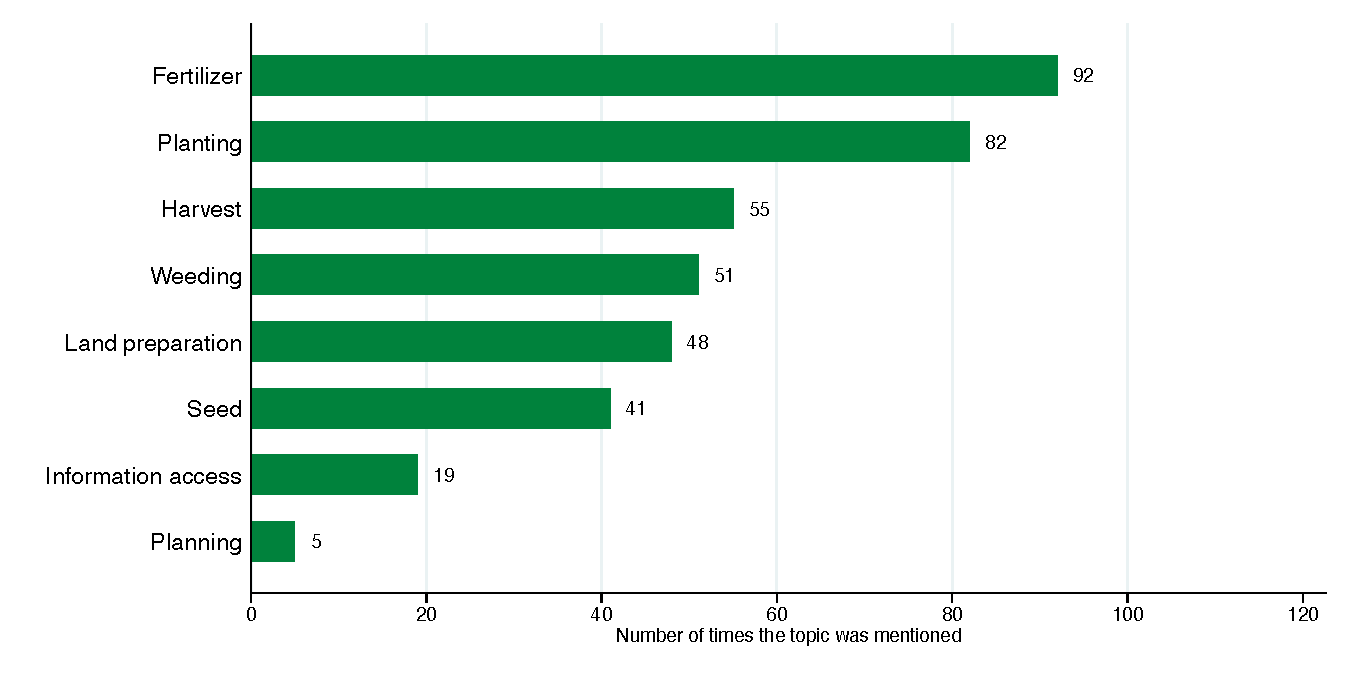
\includegraphics[width=\textwidth,height=0.60\textheight,keepaspectratio]{tmp/fig_advice_themes.pdf}
	\begin{minipage}{0.94\textwidth}
		\notefont
		Note: the open-ended reason farmers gave for their satisfaction rating (Q5), hand-coded by
		the PI, pooled over the three arms. Rainfed sites only: of the 2{,}173 rounds carrying any
		text, 302 name at least one of these eight topics (a response can name more than one).
		Bars are counts of mentions. Fertilizer, planting and weeding dominate the advice farmers
		recall.
	\end{minipage}
\end{frame}

\begin{frame}{Farmer: Production and Income}
	\centering
	\adjustbox{width=\textwidth,totalheight=0.70\textheight,keepaspectratio}{{
\def\sym#1{\ifmmode^{#1}\else\(^{#1}\)\fi}
\begin{tabular}{l*{9}{c}}
\toprule
                    &\multicolumn{1}{c}{(1)}&\multicolumn{1}{c}{(2)}&\multicolumn{1}{c}{(3)}&\multicolumn{1}{c}{(4)}&\multicolumn{1}{c}{(5)}&\multicolumn{1}{c}{(6)}&\multicolumn{1}{c}{(7)}&\multicolumn{1}{c}{(8)}&\multicolumn{1}{c}{(9)}\\
                    &\multicolumn{1}{c}{Yield}&\multicolumn{1}{c}{Log yield}&\multicolumn{1}{c}{Crop fail}&\multicolumn{1}{c}{Income/ha}&\multicolumn{1}{c}{Log income}&\multicolumn{1}{c}{Profit/ha}&\multicolumn{1}{c}{Log profit}&\multicolumn{1}{c}{Profit excl.\ bird}&\multicolumn{1}{c}{Log profit excl.}\\
\midrule
T1: Feedback        &      -0.372         &      -0.058         &      -0.056\sym{**} &     -48.399         &       2.168         &    2650.676\sym{*}  &       3.488\sym{**} &     746.224         &       3.310\sym{*}  \\
                    &     (0.387)         &     (0.128)         &     (0.021)         &  (1309.169)         &     (1.827)         &  (1124.603)         &     (1.462)         &   (997.086)         &     (1.439)         \\
T2: Feedback+Training&      -0.358         &      -0.103         &      -0.032\sym{*}  &    -271.043         &      -0.107         &    4803.059\sym{***}&       3.716\sym{**} &    2014.714\sym{**} &       3.130\sym{**} \\
                    &     (0.342)         &     (0.116)         &     (0.017)         &  (1152.423)         &     (1.720)         &   (882.331)         &     (1.301)         &   (749.093)         &     (1.318)         \\
Stamp (GPS)         &       0.056         &      -0.002         &      -0.016         &     425.752         &      -0.686         &    3261.548         &       0.220         &    2444.711         &      -0.164         \\
                    &     (0.092)         &     (0.042)         &     (0.016)         &   (718.046)         &     (1.013)         &  (2034.732)         &     (1.188)         &  (1335.265)         &     (1.202)         \\
\midrule
T1=T2 [p]           &       0.956         &       0.543         &       0.282         &       0.819         &       0.083         &       0.284         &       0.851         &       0.358         &       0.879         \\
Ctrl mean (base)    &       0.863         &       0.499         &       0.135         &    1355.693         &       0.230         &   -1139.048         &      -2.323         &    -495.675         &      -1.968         \\
Ctrl mean (end)     &       1.438         &       0.732         &       0.067         &    2416.185         &       1.910         &   -4926.736         &      -4.659         &   -1191.023         &      -3.750         \\
Wild-boot p (T1)    &       0.626         &       0.837         &       0.252         &       0.986         &       0.768         &       0.227         &       0.334         &       0.675         &       0.350         \\
Wild-boot p (T2)    &       0.775         &       0.844         &       0.078         &       0.939         &       0.983         &       0.120         &       0.211         &       0.169         &       0.200         \\
RI p (T1)           &       0.376         &       0.669         &       0.041         &       0.962         &       0.289         &       0.047         &       0.055         &       0.519         &       0.069         \\
RI p (T2)           &       0.338         &       0.418         &       0.108         &       0.820         &       0.941         &       0.000         &       0.033         &       0.020         &       0.059         \\
Obs                 &         373         &         373         &         373         &         373         &         373         &         373         &         373         &         373         &         373         \\
\bottomrule
\end{tabular}
}
}
	\begin{minipage}{0.94\textwidth}
		\notefont
		Note: ANCOVA with region FE and baseline-outcome control; SE clustered at district.
		\textbf{Income} $=$ value of output at district-median prices $-$ paid-out costs (seed,
		fertilizer, agro-chemicals, machinery services, hired labor, \emph{and what tenants pay for
		the land} --- a share of gross output for share croppers, cash or in-kind rent otherwise;
		about a third of the sample rents, and share croppers hand over a median 30\% of output);
		\textbf{profit} $=$ income
		$-$ the imputed value of own resources, here family labor valued at the district
		\emph{median} hired wage ((cash $+$ in-kind payments) $/$ hired man-days, genders pooled,
		per wave). Own machinery, recycled seed and manure are not imputed, so profit is an upper
		bound on the full-cost measure. Columns (8)--(9) exclude the family days spent on bird
		scaring, which absorb about half of all family labor. Crop failure $=0$ output, so income
		and profit can be negative; logs use the inverse hyperbolic sine. Wild-boot (Webb,
		9{,}999) and RI (1{,}000) $p$-values reported. ***, **, * : 1, 5, 10\%.
	\end{minipage}
\end{frame}

\begin{frame}{Farmer: Production and Income (controlling for technology)}
	\centering
	\adjustbox{width=\textwidth,totalheight=0.70\textheight,keepaspectratio}{{
\def\sym#1{\ifmmode^{#1}\else\(^{#1}\)\fi}
\begin{tabular}{l*{9}{c}}
\toprule
                    &\multicolumn{1}{c}{(1)}&\multicolumn{1}{c}{(2)}&\multicolumn{1}{c}{(3)}&\multicolumn{1}{c}{(4)}&\multicolumn{1}{c}{(5)}&\multicolumn{1}{c}{(6)}&\multicolumn{1}{c}{(7)}&\multicolumn{1}{c}{(8)}&\multicolumn{1}{c}{(9)}\\
                    &\multicolumn{1}{c}{Yield}&\multicolumn{1}{c}{Log yield}&\multicolumn{1}{c}{Crop fail}&\multicolumn{1}{c}{Income/ha}&\multicolumn{1}{c}{Log income}&\multicolumn{1}{c}{Profit/ha}&\multicolumn{1}{c}{Log profit}&\multicolumn{1}{c}{Profit excl.\ bird}&\multicolumn{1}{c}{Log profit excl.}\\
\midrule
T1: Feedback        &      -0.279         &      -0.043         &      -0.054\sym{**} &     148.202         &       1.742         &    2618.249\sym{***}&       3.179\sym{**} &     576.538         &       2.642\sym{*}  \\
                    &     (0.283)         &     (0.098)         &     (0.018)         &  (1028.191)         &     (1.743)         &   (614.099)         &     (1.231)         &   (778.346)         &     (1.368)         \\
T2: Feedback+Training&      -0.371         &      -0.116         &      -0.036\sym{*}  &    -450.733         &      -0.617         &    2766.374\sym{**} &       2.569         &    1036.788         &       1.916         \\
                    &     (0.275)         &     (0.098)         &     (0.017)         &  (1010.735)         &     (1.696)         &   (792.257)         &     (1.359)         &   (694.694)         &     (1.476)         \\
Stamp (GPS)         &       0.112         &       0.016         &      -0.018         &     664.138         &      -0.477         &    3092.517         &       0.340         &    2750.455         &       0.019         \\
                    &     (0.118)         &     (0.048)         &     (0.019)         &   (889.139)         &     (1.217)         &  (1889.756)         &     (1.272)         &  (1706.925)         &     (1.245)         \\
Any improved variety (=1)&      -0.075         &      -0.010         &      -0.010         &      61.889         &       0.345         &   -1315.951         &      -0.038         &     568.603         &       0.270         \\
                    &     (0.125)         &     (0.052)         &     (0.014)         &   (994.861)         &     (1.141)         &  (1848.294)         &     (1.318)         &  (1600.407)         &     (1.164)         \\
Certified seed (=1) &       0.336\sym{**} &       0.068\sym{***}&       0.007         &    1925.041\sym{**} &      -0.459         &    7552.767\sym{***}&       3.293\sym{**} &    5113.109\sym{***}&       1.887\sym{*}  \\
                    &     (0.103)         &     (0.018)         &     (0.026)         &   (785.077)         &     (0.955)         &  (1640.068)         &     (1.082)         &  (1260.599)         &     (0.834)         \\
Seed treatment (=1) &      -0.244         &      -0.080         &      -0.010         &   -1631.029         &      -0.859         &   -6871.212\sym{**} &      -3.275\sym{**} &   -6138.135\sym{**} &      -3.619\sym{**} \\
                    &     (0.274)         &     (0.081)         &     (0.019)         &  (1388.695)         &     (0.696)         &  (2168.662)         &     (0.953)         &  (2071.567)         &     (1.498)         \\
Dibbling (=1)       &       0.118         &       0.055         &      -0.013         &     877.254         &       1.699         &    1373.379         &       1.466         &     506.786         &       1.393         \\
                    &     (0.156)         &     (0.048)         &     (0.017)         &   (935.935)         &     (1.601)         &  (2347.111)         &     (1.456)         &  (2121.841)         &     (1.105)         \\
Transplant in row (=1)&       0.117         &      -0.032         &       0.020         &     302.124         &      -0.303         &   -3917.934         &      -2.155         &    1241.906         &      -1.984         \\
                    &     (0.243)         &     (0.086)         &     (0.047)         &  (1113.993)         &     (1.612)         &  (6243.599)         &     (2.034)         &  (2063.920)         &     (2.307)         \\
Bunds construction (=1)&       0.445\sym{**} &       0.137\sym{**} &       0.019         &    2083.296         &       2.764\sym{*}  &    3404.995         &       3.171         &    2910.321\sym{*}  &       2.647         \\
                    &     (0.185)         &     (0.047)         &     (0.020)         &  (1478.543)         &     (1.274)         &  (2609.792)         &     (1.712)         &  (1509.383)         &     (1.549)         \\
Levelling (=1)      &       0.011         &       0.003         &      -0.001         &    -131.236         &       0.413         &     -13.945         &      -0.964         &     367.028         &      -0.572         \\
                    &     (0.189)         &     (0.063)         &     (0.017)         &   (835.268)         &     (0.789)         &  (1048.335)         &     (1.039)         &   (851.981)         &     (0.875)         \\
Fertilizer use (=1) &       0.426\sym{**} &       0.160\sym{***}&      -0.029\sym{***}&     195.572         &      -0.341         &    -969.601         &       0.533         &    -672.854         &       0.622         \\
                    &     (0.150)         &     (0.040)         &     (0.007)         &   (960.646)         &     (0.754)         &  (1386.206)         &     (0.782)         &  (1214.072)         &     (0.922)         \\
Herb/Insecticide use (=1)&       0.252\sym{*}  &       0.051         &      -0.018         &     281.054         &      -1.517\sym{**} &   -3685.318\sym{**} &      -3.260\sym{**} &    -881.781         &      -3.301\sym{**} \\
                    &     (0.124)         &     (0.053)         &     (0.025)         &   (457.828)         &     (0.587)         &  (1433.496)         &     (1.120)         &   (635.859)         &     (1.003)         \\
Machine use (=1)    &       0.113         &       0.040         &      -0.004         &     503.013         &       0.406         &    3887.798         &       2.557\sym{**} &    1139.850         &       1.989\sym{**} \\
                    &     (0.135)         &     (0.036)         &     (0.015)         &   (573.678)         &     (0.767)         &  (2072.328)         &     (0.948)         &  (1439.503)         &     (0.703)         \\
\midrule
T1=T2 [p]           &       0.639         &       0.336         &       0.424         &       0.412         &       0.139         &       0.890         &       0.558         &       0.523         &       0.523         \\
Ctrl mean (base)    &       0.863         &       0.499         &       0.135         &    1355.693         &       0.230         &   -1139.048         &      -2.323         &    -495.675         &      -1.968         \\
Ctrl mean (end)     &       1.438         &       0.732         &       0.067         &    2416.185         &       1.910         &   -4926.736         &      -4.659         &   -1191.023         &      -3.750         \\
Wild-boot p (T1)    &       0.597         &       0.840         &       0.143         &       0.942         &       0.739         &       0.071         &       0.289         &       0.638         &       0.501         \\
Wild-boot p (T2)    &       0.693         &       0.709         &       0.100         &       0.876         &       0.925         &       0.086         &       0.287         &       0.279         &       0.579         \\
RI p (T1)           &       0.340         &       0.682         &       0.023         &       0.905         &       0.340         &       0.002         &       0.040         &       0.523         &       0.093         \\
RI p (T2)           &       0.218         &       0.293         &       0.070         &       0.671         &       0.720         &       0.009         &       0.097         &       0.191         &       0.236         \\
Obs                 &         373         &         373         &         373         &         373         &         373         &         373         &         373         &         373         &         373         \\
\bottomrule
\end{tabular}
}
}
	\begin{minipage}{0.94\textwidth}
		\notefont
		Note: same ANCOVA as the previous slide, adding the endline management
		practices and input dummies as regressors, so the treatment coefficients are
		conditional on adoption and the practice rows show how each technology correlates
		with output. \emph{Caveat}: adoption is measured after the intervention, so these
		are potentially ``bad controls'' --- the practice rows are correlations, not causal
		effects, and the treatment rows are net of any adoption channel. Region FE and
		baseline-outcome control; SE clustered at district; wild-boot (Webb, 9{,}999) and
		RI (1{,}000) $p$-values. ***, **, * : 1, 5, 10\%.
	\end{minipage}
\end{frame}

\begin{frame}{Farmer: Inputs}
	\centering
	\adjustbox{width=\textwidth,totalheight=0.70\textheight,keepaspectratio}{{
\def\sym#1{\ifmmode^{#1}\else\(^{#1}\)\fi}
\begin{tabular}{l*{7}{c}}
\toprule
                    &\multicolumn{1}{c}{(1)}&\multicolumn{1}{c}{(2)}&\multicolumn{1}{c}{(3)}&\multicolumn{1}{c}{(4)}&\multicolumn{1}{c}{(5)}&\multicolumn{1}{c}{(6)}&\multicolumn{1}{c}{(7)}\\
                    &\multicolumn{1}{c}{Seed qty}&\multicolumn{1}{c}{Fert use}&\multicolumn{1}{c}{Herb use}&\multicolumn{1}{c}{Machine}&\multicolumn{1}{c}{Hired lab}&\multicolumn{1}{c}{Family lab}&\multicolumn{1}{c}{Family excl.\ bird}\\
\midrule
T1: Feedback        &     -14.143\sym{**} &       0.024         &      -0.135\sym{***}&       0.032         &      30.563\sym{***}&     -14.146         &       3.309         \\
                    &     (4.533)         &     (0.053)         &     (0.029)         &     (0.067)         &     (3.241)         &    (16.952)         &     (6.164)         \\
T2: Feedback+Training&     -22.385\sym{***}&      -0.009         &      -0.100\sym{***}&       0.137\sym{**} &      19.862\sym{***}&     -50.741\sym{**} &     -20.206\sym{***}\\
                    &     (4.808)         &     (0.048)         &     (0.026)         &     (0.057)         &     (2.891)         &    (15.742)         &     (5.281)         \\
Stamp (GPS)         &      -3.079         &      -0.025         &      -0.063         &       0.044         &      -0.965         &     -38.318         &     -25.892         \\
                    &     (4.671)         &     (0.072)         &     (0.093)         &     (0.060)         &     (6.187)         &    (25.004)         &    (13.954)         \\
\midrule
T1=T2 [p]           &       0.014         &       0.411         &       0.232         &       0.236         &       0.051         &       0.125         &       0.063         \\
Ctrl mean (base)    &      70.249         &       0.652         &       0.809         &       0.730         &      53.117         &      49.895         &      37.027         \\
Ctrl mean (end)     &      99.431         &       0.633         &       0.833         &       0.600         &      33.470         &     101.672         &      51.411         \\
Wild-boot p (T1)    &       0.179         &       0.850         &       0.177         &       0.820         &       0.056         &       0.715         &       0.737         \\
Wild-boot p (T2)    &       0.063         &       0.928         &       0.224         &       0.412         &       0.057         &       0.275         &       0.194         \\
RI p (T1)           &       0.025         &       0.663         &       0.001         &       0.663         &       0.000         &       0.493         &       0.687         \\
RI p (T2)           &       0.006         &       0.841         &       0.007         &       0.070         &       0.000         &       0.022         &       0.005         \\
Obs                 &         369         &         373         &         373         &         373         &         373         &         373         &         373         \\
\bottomrule
\end{tabular}
}
}
	\begin{minipage}{0.94\textwidth}
		\notefont
		Note: same ANCOVA specification as the previous slide (region FE,
		baseline-outcome control, SE clustered at district). Fertilizer, herbicide and machine
		use are $0/1$ indicators; hired and family labor are man-days per ha, with the last
		column netting out the family days spent on bird scaring. Wild-boot (Webb, 9{,}999)
		and RI (1{,}000) $p$-values reported. ***, **, * : 1, 5, 10\%.
	\end{minipage}
\end{frame}





\begin{frame}{Farmer: Management-Practice Adoption}
	\centering
	\adjustbox{width=\textwidth,totalheight=0.70\textheight,keepaspectratio}{{
\def\sym#1{\ifmmode^{#1}\else\(^{#1}\)\fi}
\begin{tabular}{l*{8}{c}}
\toprule
                    &\multicolumn{1}{c}{(1)}&\multicolumn{1}{c}{(2)}&\multicolumn{1}{c}{(3)}&\multicolumn{1}{c}{(4)}&\multicolumn{1}{c}{(5)}&\multicolumn{1}{c}{(6)}&\multicolumn{1}{c}{(7)}&\multicolumn{1}{c}{(8)}\\
                    &\multicolumn{1}{c}{Any improved}&\multicolumn{1}{c}{Certified}&\multicolumn{1}{c}{Seed trt}&\multicolumn{1}{c}{Dibbling}&\multicolumn{1}{c}{Row trans}&\multicolumn{1}{c}{Bunds}&\multicolumn{1}{c}{Levelling}&\multicolumn{1}{c}{No. practices}\\
\midrule
T1: Feedback        &       0.280\sym{***}&      -0.156\sym{*}  &      -0.127         &       0.028         &      -0.019         &      -0.063         &      -0.012         &      -0.014         \\
                    &     (0.052)         &     (0.074)         &     (0.106)         &     (0.042)         &     (0.011)         &     (0.121)         &     (0.070)         &     (0.309)         \\
T2: Feedback+Training&      -0.009         &      -0.086         &      -0.138         &      -0.046         &      -0.062\sym{***}&       0.052         &       0.061         &      -0.197         \\
                    &     (0.041)         &     (0.067)         &     (0.098)         &     (0.031)         &     (0.015)         &     (0.105)         &     (0.063)         &     (0.278)         \\
Stamp (GPS)         &      -0.031         &       0.041         &       0.088         &      -0.074         &      -0.024         &      -0.051         &       0.099         &       0.055         \\
                    &     (0.031)         &     (0.036)         &     (0.063)         &     (0.103)         &     (0.035)         &     (0.037)         &     (0.093)         &     (0.125)         \\
\midrule
T1=T2 [p]           &       0.014         &       0.279         &       0.886         &       0.334         &       0.050         &       0.186         &       0.108         &       0.384         \\
Ctrl mean (base)    &       0.472         &       0.157         &       0.180         &       0.045         &       0.079         &       0.067         &       0.303         &       1.303         \\
Ctrl mean (end)     &       0.411         &       0.144         &       0.333         &       0.033         &       0.067         &       0.133         &       0.433         &       1.556         \\
Wild-boot p (T1)    &       0.086         &       0.127         &       0.701         &       0.753         &       0.076         &       0.827         &       0.946         &       0.989         \\
Wild-boot p (T2)    &       0.898         &       0.686         &       0.703         &       0.368         &       0.165         &       0.830         &       0.677         &       0.882         \\
RI p (T1)           &       0.002         &       0.089         &       0.307         &       0.537         &       0.113         &       0.631         &       0.882         &       0.964         \\
RI p (T2)           &       0.834         &       0.235         &       0.242         &       0.202         &       0.001         &       0.636         &       0.342         &       0.538         \\
Obs                 &         373         &         373         &         373         &         373         &         373         &         373         &         373         &         373         \\
\bottomrule
\end{tabular}
}
}
	\begin{minipage}{0.94\textwidth}
		\notefont
		Note: ANCOVA with region FE and baseline-outcome control; SE clustered at district.
		No.\ practices $=$ count of the seven practices adopted (0--7). Seed-variety and
		certified-seed measures use the original endline export. ***, **, * : 1, 5, 10\%.
	\end{minipage}
\end{frame}

\begin{frame}{Farmer: Labour by Who Does the Work and by Operation}
	\centering
	{\notefont\textbf{Man-days per hectare, male vs female}}\\[1pt]
	\adjustbox{width=\textwidth,totalheight=0.30\textheight,keepaspectratio}{{
\def\sym#1{\ifmmode^{#1}\else\(^{#1}\)\fi}
\begin{tabular}{l*{8}{c}}
\toprule
                    &\multicolumn{3}{c}{Family labour}                                &\multicolumn{3}{c}{Hired labour}                                 &\multicolumn{2}{c}{Excl.\ crop failure}    \\\cmidrule(lr){2-4}\cmidrule(lr){5-7}\cmidrule(lr){8-9}
                    &\multicolumn{1}{c}{(1)}&\multicolumn{1}{c}{(2)}&\multicolumn{1}{c}{(3)}&\multicolumn{1}{c}{(4)}&\multicolumn{1}{c}{(5)}&\multicolumn{1}{c}{(6)}&\multicolumn{1}{c}{(7)}&\multicolumn{1}{c}{(8)}\\
                    &\multicolumn{1}{c}{All}&\multicolumn{1}{c}{Male}&\multicolumn{1}{c}{Female}&\multicolumn{1}{c}{All}&\multicolumn{1}{c}{Male}&\multicolumn{1}{c}{Female}&\multicolumn{1}{c}{Family}&\multicolumn{1}{c}{Hired}\\
\midrule
T1: Feedback        &      -14.15         &       -2.42         &      -11.71         &       30.56\sym{***}&        2.76\sym{***}&       28.76\sym{***}&      -16.13         &       29.47\sym{***}\\
                    &     (16.95)         &      (9.40)         &      (8.03)         &      (3.24)         &      (0.50)         &      (2.89)         &     (17.03)         &      (3.75)         \\
T2: Feedback+Training&      -50.74\sym{**} &      -26.69\sym{**} &      -23.55\sym{**} &       19.86\sym{***}&       -8.35\sym{***}&       27.77\sym{***}&      -51.32\sym{**} &       18.71\sym{***}\\
                    &     (15.74)         &      (8.85)         &      (7.02)         &      (2.89)         &      (0.52)         &      (2.39)         &     (15.53)         &      (3.38)         \\
\midrule
T1=T2 [p]           &       0.125         &       0.122         &       0.158         &       0.051         &       0.000         &       0.725         &       0.131         &       0.049         \\
Ctrl mean           &      101.07         &       60.18         &       40.89         &       33.57         &       19.21         &       14.35         &      107.37         &       35.76         \\
Obs                 &         373         &         373         &         373         &         373         &         373         &         373         &         361         &         361         \\
\bottomrule
\end{tabular}
}
}\\[4pt]
	{\notefont\textbf{Man-days per hectare, by farm operation}}\\[1pt]
	\adjustbox{width=\textwidth,totalheight=0.30\textheight,keepaspectratio}{{
\def\sym#1{\ifmmode^{#1}\else\(^{#1}\)\fi}
\begin{tabular}{l*{12}{c}}
\toprule
                    &\multicolumn{6}{c}{Family labour (man-days/ha)}                                                                                    &\multicolumn{6}{c}{Hired labour (man-days/ha)}                                                                                     \\\cmidrule(lr){2-7}\cmidrule(lr){8-13}
                    &\multicolumn{1}{c}{(1)}&\multicolumn{1}{c}{(2)}&\multicolumn{1}{c}{(3)}&\multicolumn{1}{c}{(4)}&\multicolumn{1}{c}{(5)}&\multicolumn{1}{c}{(6)}&\multicolumn{1}{c}{(7)}&\multicolumn{1}{c}{(8)}&\multicolumn{1}{c}{(9)}&\multicolumn{1}{c}{(10)}&\multicolumn{1}{c}{(11)}&\multicolumn{1}{c}{(12)}\\
                    &\multicolumn{1}{c}{Land prep}&\multicolumn{1}{c}{Transpl./sow}&\multicolumn{1}{c}{Weeding}&\multicolumn{1}{c}{Bird}&\multicolumn{1}{c}{Harvest}&\multicolumn{1}{c}{Thresh}&\multicolumn{1}{c}{Land prep}&\multicolumn{1}{c}{Transpl./sow}&\multicolumn{1}{c}{Weeding}&\multicolumn{1}{c}{Bird}&\multicolumn{1}{c}{Harvest}&\multicolumn{1}{c}{Thresh}\\
\midrule
T1: Feedback        &       -2.33\sym{***}&        5.12\sym{***}&        1.00\sym{*}  &      -18.01         &        3.85         &       -0.82         &        3.72\sym{*}  &        0.36\sym{***}&       -0.60\sym{**} &        0.52         &       25.30\sym{***}&        0.25         \\
                    &      (0.50)         &      (1.02)         &      (0.47)         &     (11.49)         &      (3.70)         &      (2.78)         &      (1.67)         &      (0.09)         &      (0.20)         &      (0.31)         &      (3.40)         &      (0.36)         \\
T2: Feedback+Training&       -3.20\sym{***}&       -7.76\sym{***}&       -0.33         &      -30.72\sym{**} &       -4.30         &       -3.10         &       -1.68         &       -2.66\sym{***}&       -1.02\sym{***}&        2.97\sym{***}&       17.71\sym{***}&        0.77\sym{**} \\
                    &      (0.71)         &      (0.84)         &      (0.36)         &     (10.76)         &      (3.32)         &      (2.14)         &      (1.53)         &      (0.37)         &      (0.17)         &      (0.36)         &      (0.98)         &      (0.28)         \\
\midrule
T1=T2 [p]           &       0.207         &       0.000         &       0.083         &       0.243         &       0.280         &       0.611         &       0.001         &       0.000         &       0.078         &       0.008         &       0.107         &       0.179         \\
Ctrl mean           &       10.40         &        7.00         &        1.30         &       50.39         &       16.33         &       13.09         &        7.91         &        2.36         &        1.59         &        0.82         &       15.68         &        4.36         \\
Obs                 &         373         &         373         &         373         &         373         &         373         &         373         &         373         &         373         &         373         &         373         &         373         &         373         \\
\bottomrule
\end{tabular}
}
}
	\begin{minipage}{0.94\textwidth}
		\notefont
		Note: man-days per hectare. Same ANCOVA and same sample as the main tables (arms, stamp,
		the same outcome at baseline, province FE; SE clustered at district; the two
		irrigation schemes excluded, as everywhere). 
		In the top panel, columns (7)--(8) drop the 12 households that
		harvested nothing at endline. In the bottom panel, nursery, irrigation and spraying are
		omitted --- each is under 2\% of total labour.
		\par The rise in hired female labour attributes to harvest work: the
		harvest-only effect is $+26.6$ days/ha for T1 (92.6\% of total effect) and $+22.2$ for T2 (80.0\%).
		***, **, * : 1, 5, 10\%.
	\end{minipage}
\end{frame}


% ======================= APPENDIX =======================
\appendix
\begin{frame}[plain]
	\vfill
	\centering
	{\Huge\bfseries\textcolor{myGreen}{Appendix}}
	\vfill
\end{frame}

\begin{frame}{Appendix: Farmer Knowledge --- Correct-Practice Responses}
	\centering
	\adjustbox{width=\textwidth,totalheight=0.70\textheight,keepaspectratio}{{
\def\sym#1{\ifmmode^{#1}\else\(^{#1}\)\fi}
\begin{tabular}{l*{7}{c}}
\toprule
                    &\multicolumn{1}{c}{(1)}&\multicolumn{1}{c}{(2)}&\multicolumn{1}{c}{(3)}&\multicolumn{1}{c}{(4)}&\multicolumn{1}{c}{(5)}&\multicolumn{1}{c}{(6)}&\multicolumn{1}{c}{(7)}\\
                    &\multicolumn{1}{c}{Water: grow}&\multicolumn{1}{c}{Water: repr}&\multicolumn{1}{c}{Water: mat}&\multicolumn{1}{c}{Drying}&\multicolumn{1}{c}{Harvest}&\multicolumn{1}{c}{Moisture}&\multicolumn{1}{c}{Threshing}\\
\midrule
T1: Feedback        &       0.060         &      -0.133\sym{***}&       0.043         &       0.119\sym{*}  &       0.050         &       0.029         &      -0.085\sym{***}\\
                    &     (0.037)         &     (0.032)         &     (0.045)         &     (0.054)         &     (0.058)         &     (0.016)         &     (0.017)         \\
T2: Feedback+Training&      -0.083\sym{**} &      -0.090\sym{**} &       0.047         &       0.013         &      -0.005         &       0.032\sym{*}  &      -0.082\sym{***}\\
                    &     (0.035)         &     (0.030)         &     (0.039)         &     (0.049)         &     (0.047)         &     (0.014)         &     (0.015)         \\
Stamp (GPS)         &      -0.069         &      -0.014         &      -0.040         &       0.001         &       0.011         &       0.002         &      -0.098\sym{**} \\
                    &     (0.047)         &     (0.081)         &     (0.061)         &     (0.047)         &     (0.068)         &     (0.040)         &     (0.028)         \\
\midrule
T1=T2 [p]           &       0.000         &       0.120         &       0.930         &       0.065         &       0.475         &       0.874         &       0.913         \\
Ctrl mean (base)    &       0.101         &       0.225         &       0.146         &       0.079         &       0.506         &       0.191         &       0.719         \\
Ctrl mean (end)     &       0.344         &       0.411         &       0.167         &       0.889         &       0.433         &       0.156         &       0.911         \\
Wild-boot p (T1)    &       0.557         &       0.081         &       0.710         &       0.125         &       0.680         &       0.355         &       0.122         \\
Wild-boot p (T2)    &       0.529         &       0.278         &       0.513         &       0.921         &       0.946         &       0.218         &       0.110         \\
RI p (T1)           &       0.167         &       0.008         &       0.387         &       0.055         &       0.403         &       0.127         &       0.000         \\
RI p (T2)           &       0.059         &       0.030         &       0.284         &       0.836         &       0.902         &       0.043         &       0.001         \\
Obs                 &         373         &         373         &         373         &         373         &         373         &         373         &         373         \\
\bottomrule
\end{tabular}
}
}
	\begin{minipage}{0.94\textwidth}
		\notefont
		Note: each outcome $=1$ if the farmer's \emph{self-reported practice} matches the
		recommended level (QY1.4: ``what did you do'' questions scored against recommendations
		--- a knowledge-in-practice proxy rather than a quiz). Items and correct answers:
		water level at vegetative growth $=$ 2--3 cm; at reproductive (panicle) stage $=$
		5--10 cm; at maturity/ripening $=$ 1 cm; field drained \emph{two weeks} before harvest;
		harvest when 81--90\% of grains are yellowish; grain ``slightly firm to bite'' before
		storage; threshing done on a tarpaulin. ANCOVA as in the main tables; SE clustered at
		district; wild-boot (Webb, 9{,}999) and RI (1{,}000) $p$-values. ***, **, * : 1, 5, 10\%.
	\end{minipage}
\end{frame}


\begin{frame}{Appendix: AEA Effort --- GPS-Stamp Visit Log vs Reported Visits}
	\centering
	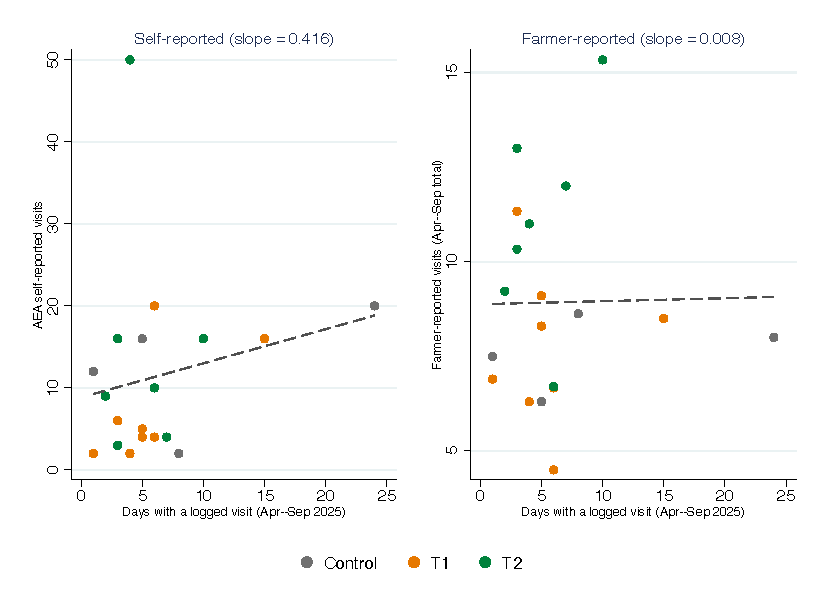
\includegraphics[height=0.62\textheight,keepaspectratio]{tmp/fig_stamp_visits.pdf}
	\begin{minipage}{0.94\textwidth}
		\notefont
		Note: 357 geo-tagged contacts logged by 19 stamp-arm AEAs, Apr--Sep 2025; logs are
		AEA-submitted, so they bound visits from below. The logged activity is unrelated to
		self-reported visits (Spearman $0.25$, $p=.30$) or farmer-reported visits
		($-0.02$, $p=.94$).
	\end{minipage}
\end{frame}

\begin{frame}{Appendix: AEA Effort --- What the Logged Visits Look Like}
	\centering
	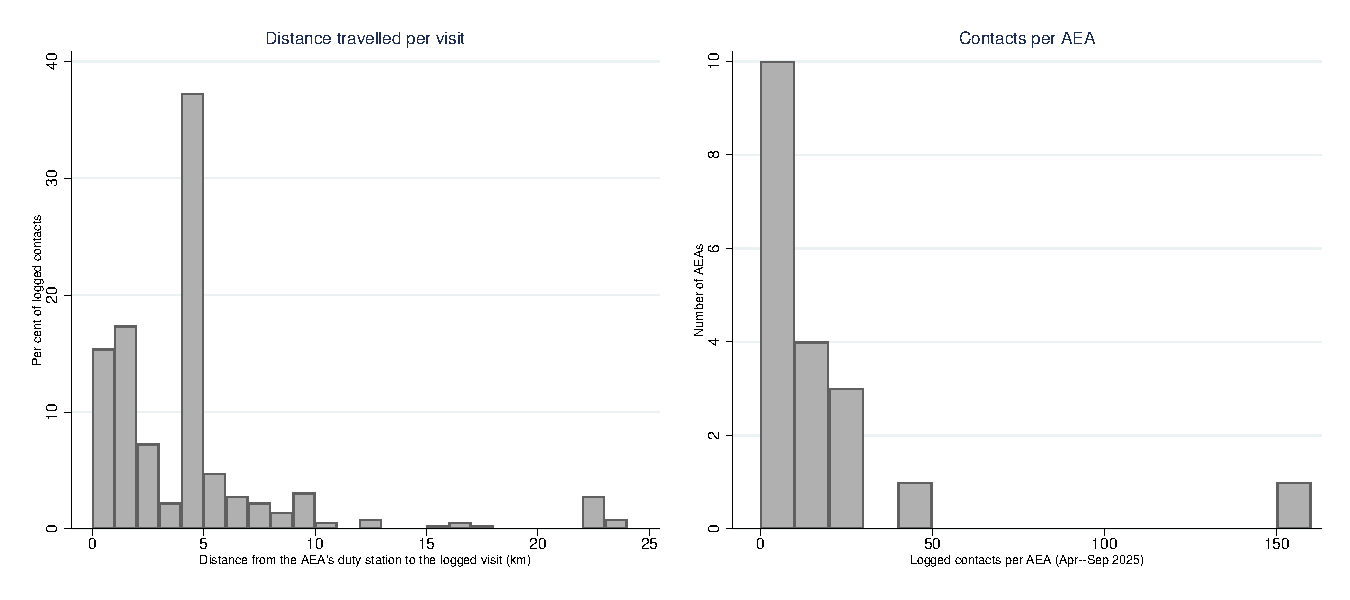
\includegraphics[width=\textwidth,keepaspectratio]{tmp/fig_stamp_activity.pdf}
	\begin{minipage}{0.94\textwidth}
		\notefont
		Note: 357 logged contacts, 19 AEAs. Distance travelled: mean 4.5\,km, median 4.9,
		maximum 23.5. The most active AEA logged 43.7\% of all contacts, the least active one
		visit in six months.
	\end{minipage}
\end{frame}

\begin{frame}{Prosocialness Answers: Baseline vs Endline (AEA)}
\begin{figure}
	\centering
	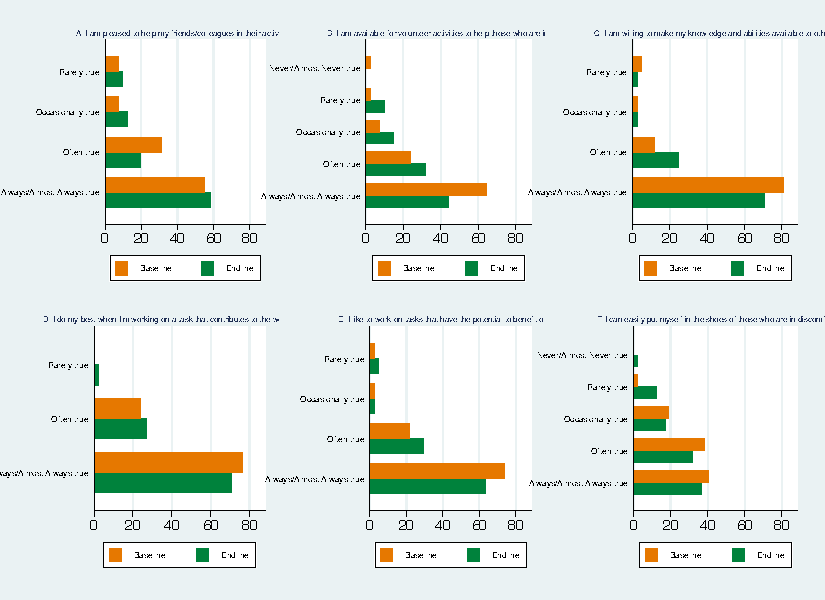
\includegraphics[height=0.78\textheight,keepaspectratio]{tmp/prosocial_be.pdf}
\end{figure}
\end{frame}

\begin{frame}{Locus of Control Answers (A--E): Baseline vs Endline (AEA)}
\begin{figure}
	\centering
	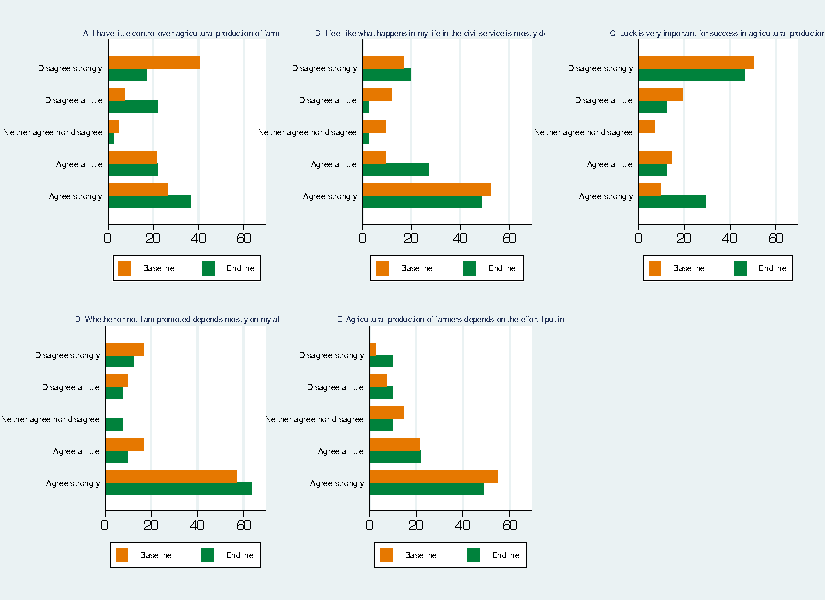
\includegraphics[height=0.78\textheight,keepaspectratio]{tmp/locus1_be.pdf}
\end{figure}
\end{frame}

\begin{frame}{Locus of Control Answers (F--J): Baseline vs Endline (AEA)}
\begin{figure}
	\centering
	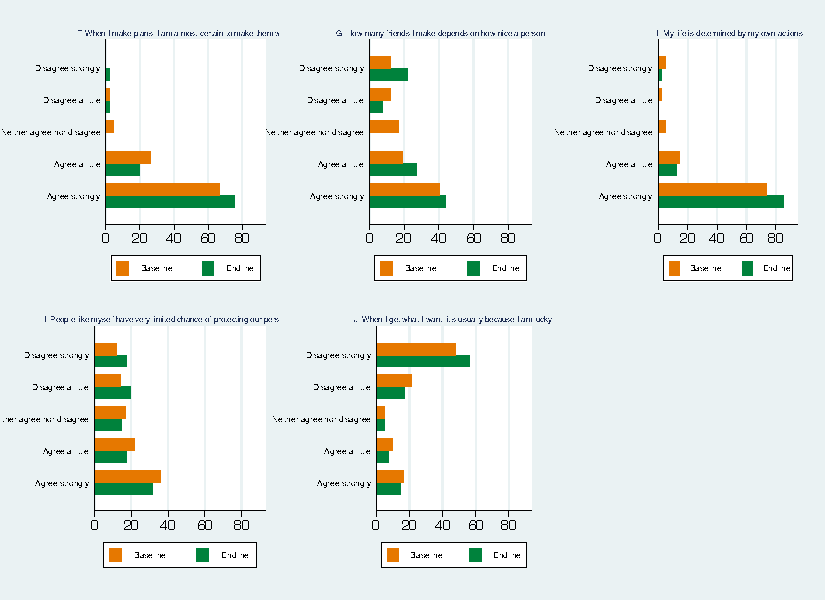
\includegraphics[height=0.78\textheight,keepaspectratio]{tmp/locus2_be.pdf}
\end{figure}
\end{frame}



\begin{frame}{Appendix: Sampling-Weighted Robustness (Production)}
	\centering
	\adjustbox{width=\textwidth,totalheight=0.70\textheight,keepaspectratio}{{
\def\sym#1{\ifmmode^{#1}\else\(^{#1}\)\fi}
\begin{tabular}{l*{16}{c}}
\toprule
                    &\multicolumn{1}{c}{(1)}&\multicolumn{1}{c}{(2)}&\multicolumn{1}{c}{(3)}&\multicolumn{1}{c}{(4)}&\multicolumn{1}{c}{(5)}&\multicolumn{1}{c}{(6)}&\multicolumn{1}{c}{(7)}&\multicolumn{1}{c}{(8)}&\multicolumn{1}{c}{(9)}&\multicolumn{1}{c}{(10)}&\multicolumn{1}{c}{(11)}&\multicolumn{1}{c}{(12)}&\multicolumn{1}{c}{(13)}&\multicolumn{1}{c}{(14)}&\multicolumn{1}{c}{(15)}&\multicolumn{1}{c}{(16)}\\
                    &\multicolumn{1}{c}{Revenue/ha}&\multicolumn{1}{c}{Income/ha}&\multicolumn{1}{c}{Profit/ha}&\multicolumn{1}{c}{Log profit}&\multicolumn{1}{c}{Yield}&\multicolumn{1}{c}{Log yield}&\multicolumn{1}{c}{Crop fail}&\multicolumn{1}{c}{Fert use}&\multicolumn{1}{c}{Herb use}&\multicolumn{1}{c}{Machine}&\multicolumn{1}{c}{Hired lab}&\multicolumn{1}{c}{Family lab}&\multicolumn{1}{c}{lnrincome}&\multicolumn{1}{c}{fincnb\_ha}&\multicolumn{1}{c}{lfincnb}&\multicolumn{1}{c}{famdnb\_ha}\\
\midrule
T1: Feedback        &     245.353         &     654.066         &    1260.677         &       7.143\sym{*}  &      -0.230         &       0.027         &      -0.049\sym{***}&       0.154\sym{***}&      -0.356\sym{***}&      -0.096\sym{**} &      46.559\sym{**} &     -18.671         &       5.493         &    1491.504         &       6.381         &      -7.794         \\
                    &  (3476.089)         &  (2548.681)         &  (2323.300)         &     (3.144)         &     (0.546)         &     (0.135)         &     (0.013)         &     (0.026)         &     (0.041)         &     (0.036)         &    (18.528)         &    (13.230)         &     (3.114)         &  (2425.613)         &     (3.400)         &    (10.969)         \\
T2: Feedback+Training&    3362.644         &    2018.416         &    7051.784\sym{**} &      10.052\sym{**} &       0.046         &       0.051         &      -0.007         &      -0.067\sym{***}&      -0.234\sym{***}&       0.184\sym{***}&     -17.036         &     -51.676\sym{**} &       4.332         &    5273.410\sym{*}  &       9.334\sym{**} &     -44.961\sym{**} \\
                    &  (3926.841)         &  (2872.932)         &  (2655.228)         &     (3.471)         &     (0.638)         &     (0.161)         &     (0.018)         &     (0.018)         &     (0.056)         &     (0.032)         &    (31.890)         &    (19.198)         &     (3.683)         &  (2532.104)         &     (3.799)         &    (16.306)         \\
Stamp (GPS)         &    2415.321         &    1769.793         &    4698.240         &       2.548         &       0.383         &       0.060         &      -0.067\sym{*}  &      -0.031         &      -0.064         &      -0.028         &       2.699         &     -26.737         &      -0.196         &    3606.971         &       1.092         &     -20.991         \\
                    &  (1545.152)         &  (1240.489)         &  (3661.880)         &     (2.727)         &     (0.215)         &     (0.052)         &     (0.031)         &     (0.068)         &     (0.084)         &     (0.044)         &    (13.459)         &    (25.224)         &     (1.182)         &  (2782.366)         &     (1.313)         &    (19.180)         \\
\midrule
T1=T2 [p]           &       0.340         &       0.632         &       0.014         &       0.187         &       0.592         &       0.862         &       0.170         &       0.000         &       0.101         &       0.000         &       0.193         &       0.315         &       0.677         &       0.098         &       0.172         &       0.175         \\
Ctrl mean (base, wtd)&    7400.976         &    3177.027         &    -125.634         &       1.302         &       0.790         &       0.518         &       0.029         &       0.732         &       0.613         &       0.857         &      41.425         &      66.053         &       4.091         &     904.323         &       1.800         &      45.454         \\
Ctrl mean (end, wtd)&    5189.997         &    1412.689         &   -1971.617         &      -5.436         &       1.096         &       0.589         &       0.037         &       0.653         &       0.856         &       0.784         &      36.480         &      54.741         &      -1.018         &    -943.949         &      -4.929         &      39.911         \\
Obs                 &         373         &         373         &         373         &         373         &         373         &         373         &         373         &         373         &         373         &         373         &         373         &         373         &         373         &         373         &         373         &         373         \\
\bottomrule
\end{tabular}
}
}
	\begin{minipage}{0.94\textwidth}
		\notefont
		Note: Population-representative estimates using inverse-probability sampling weights
		(rice-farmer population $/$ baseline sample size). Region FE and baseline-outcome control;
		SE clustered at district. Income defined as in the main production table (net of family labor).
		***, **, * : 1, 5, 10\%.
	\end{minipage}
\end{frame}

\begin{frame}{Appendix: Sampling-Weighted Robustness (Practices)}
	\centering
	\adjustbox{width=\textwidth,totalheight=0.70\textheight,keepaspectratio}{{
\def\sym#1{\ifmmode^{#1}\else\(^{#1}\)\fi}
\begin{tabular}{l*{8}{c}}
\toprule
                    &\multicolumn{1}{c}{(1)}&\multicolumn{1}{c}{(2)}&\multicolumn{1}{c}{(3)}&\multicolumn{1}{c}{(4)}&\multicolumn{1}{c}{(5)}&\multicolumn{1}{c}{(6)}&\multicolumn{1}{c}{(7)}&\multicolumn{1}{c}{(8)}\\
                    &\multicolumn{1}{c}{Any improved}&\multicolumn{1}{c}{Certified}&\multicolumn{1}{c}{Seed trt}&\multicolumn{1}{c}{Dibbling}&\multicolumn{1}{c}{Row trans}&\multicolumn{1}{c}{Bunds}&\multicolumn{1}{c}{Levelling}&\multicolumn{1}{c}{No. practices}\\
\midrule
T1: Feedback        &       0.359\sym{***}&      -0.133         &       0.005         &      -0.025         &      -0.016         &      -0.036         &       0.007         &       0.235         \\
                    &     (0.065)         &     (0.132)         &     (0.092)         &     (0.083)         &     (0.019)         &     (0.140)         &     (0.068)         &     (0.377)         \\
T2: Feedback+Training&       0.066         &       0.118         &       0.076         &       0.103         &      -0.045         &       0.100         &       0.203\sym{**} &       0.667         \\
                    &     (0.134)         &     (0.150)         &     (0.099)         &     (0.133)         &     (0.029)         &     (0.163)         &     (0.082)         &     (0.451)         \\
Stamp (GPS)         &       0.101         &       0.211         &       0.058         &       0.057         &      -0.022         &      -0.090\sym{**} &       0.258         &       0.484\sym{*}  \\
                    &     (0.054)         &     (0.188)         &     (0.066)         &     (0.097)         &     (0.025)         &     (0.038)         &     (0.152)         &     (0.223)         \\
\midrule
T1=T2 [p]           &       0.181         &       0.020         &       0.293         &       0.546         &       0.545         &       0.325         &       0.004         &       0.251         \\
Ctrl mean (base, wtd)&       0.277         &       0.130         &       0.056         &       0.008         &       0.032         &       0.023         &       0.162         &       0.688         \\
Ctrl mean (end, wtd)&       0.229         &       0.057         &       0.140         &       0.003         &       0.028         &       0.057         &       0.546         &       1.060         \\
Obs                 &         373         &         373         &         373         &         373         &         373         &         373         &         373         &         373         \\
\bottomrule
\end{tabular}
}
}
	\begin{minipage}{0.94\textwidth}
		\notefont
		Note: Population-representative estimates using inverse-probability sampling weights
		(rice-farmer population $/$ baseline sample size). Region FE and baseline-outcome control;
		SE clustered at district. ***, **, * : 1, 5, 10\%.
	\end{minipage}
\end{frame}

\begin{frame}{Appendix: Dispersion Effects (Glejser)}
	\centering
	\adjustbox{width=\textwidth,totalheight=0.70\textheight,keepaspectratio}{{
\def\sym#1{\ifmmode^{#1}\else\(^{#1}\)\fi}
\begin{tabular}{l*{4}{c}}
\toprule
                    &\multicolumn{1}{c}{(1)}&\multicolumn{1}{c}{(2)}&\multicolumn{1}{c}{(3)}&\multicolumn{1}{c}{(4)}\\
                    &\multicolumn{1}{c}{Yield}&\multicolumn{1}{c}{Log yield}&\multicolumn{1}{c}{Income/ha}&\multicolumn{1}{c}{Log income}\\
\midrule
T1: Feedback        &      -0.350         &      -0.050         &   -2676.221         &       0.973         \\
                    &     (0.265)         &     (0.072)         &  (2244.359)         &     (0.814)         \\
T2: Feedback+Training&      -0.169         &      -0.001         &   -2515.900         &       1.446\sym{*}  \\
                    &     (0.235)         &     (0.065)         &  (2014.489)         &     (0.717)         \\
Stamp (GPS)         &       0.042         &       0.008         &   -2463.424         &       0.245         \\
                    &     (0.088)         &     (0.024)         &  (1565.989)         &     (0.223)         \\
\midrule
T1=T2 [p]           &       0.432         &       0.400         &       0.920         &       0.529         \\
Ctrl mean |resid|   &       0.888         &       0.302         &    7552.770         &       6.462         \\
Wild-boot p (T1)    &       0.517         &       0.739         &       0.595         &       0.651         \\
Wild-boot p (T2)    &       0.816         &       0.996         &       0.724         &       0.175         \\
Obs                 &         373         &         373         &         373         &         373         \\
\bottomrule
\end{tabular}
}
}
	\begin{minipage}{0.94\textwidth}
		\notefont
		Note: Glejser test --- absolute residuals from the main ANCOVA regressed on
		treatment; negative coefficients $=$ lower dispersion. Wild-boot (Webb, 9{,}999)
		$p$-values. NB: the two extreme hired-labor records (297{,}000 / 252{,}000 GHS;
		hhID 311/381) behind the earlier variance discussion were in-kind data-entry errors,
		corrected in the revised labor file used throughout (current maximum 25{,}600 GHS).
		***, **, * : 1, 5, 10\%.
	\end{minipage}
\end{frame}

\begin{frame}{Appendix: Profit Excluding Bird-Scaring Labor}
	\centering
	\adjustbox{width=\textwidth,totalheight=0.70\textheight,keepaspectratio}{{
\def\sym#1{\ifmmode^{#1}\else\(^{#1}\)\fi}
\begin{tabular}{l*{3}{c}}
\toprule
                    &\multicolumn{1}{c}{(1)}&\multicolumn{1}{c}{(2)}&\multicolumn{1}{c}{(3)}\\
                    &\multicolumn{1}{c}{Profit excl. bird}&\multicolumn{1}{c}{Log profit excl. bird}&\multicolumn{1}{c}{Bird days/ha}\\
\midrule
T1: Feedback        &     746.224         &       3.310\sym{*}  &     -18.007         \\
                    &   (997.086)         &     (1.439)         &    (11.487)         \\
T2: Feedback+Training&    2014.714\sym{**} &       3.130\sym{**} &     -30.717\sym{**} \\
                    &   (749.093)         &     (1.318)         &    (10.755)         \\
Stamp (GPS)         &    2444.711         &      -0.164         &     -11.311         \\
                    &  (1335.265)         &     (1.202)         &    (15.989)         \\
\midrule
T1=T2 [p]           &       0.358         &       0.879         &       0.243         \\
Ctrl mean (base)    &    -495.675         &      -1.968         &      12.867         \\
Ctrl mean (end)     &   -1191.023         &      -3.750         &      50.261         \\
Wild-boot p (T1)    &       0.675         &       0.350         &       0.591         \\
Wild-boot p (T2)    &       0.169         &       0.200         &       0.398         \\
RI p (T1)           &       0.519         &       0.069         &       0.172         \\
RI p (T2)           &       0.020         &       0.059         &       0.011         \\
Obs                 &         373         &         373         &         373         \\
\bottomrule
\end{tabular}
}
}
	\begin{minipage}{0.94\textwidth}
		\notefont
		Note: bird scaring is a distinct operation in the labor module and absorbs many
		low-intensity days spent guarding the field, so valuing it at the hired wage is
		questionable. Columns (1)--(2) recompute profit deducting family labor
		\emph{excluding} bird-scaring days; column (3) is bird-scaring family labor itself.
		Control households devote 52.3 days/ha to bird scaring --- about half of all family
		labor (50.3\%) --- and excluding it turns the control-group profit from $-3{,}398$ to
		$+600$ GHS/ha. ANCOVA as in the main table; SE clustered at district; wild-boot
		(Webb, 9{,}999) and RI (1{,}000) $p$-values. ***, **, * : 1, 5, 10\%.
	\end{minipage}
\end{frame}



% ---- A1. FB/TR reparameterization ----
\begin{frame}{Appendix: FB/TR --- Bi-weekly Effort}
	\centering
	\adjustbox{width=\textwidth,totalheight=0.70\textheight,keepaspectratio}{{
\def\sym#1{\ifmmode^{#1}\else\(^{#1}\)\fi}
\begin{tabular}{l*{8}{c}}
\toprule
                    &\multicolumn{4}{c}{All rounds (Apr--Sep)}                                              &\multicolumn{4}{c}{Planting window (05-1--06-2)}                                       \\\cmidrule(lr){2-5}\cmidrule(lr){6-9}
                    &\multicolumn{1}{c}{(1)}&\multicolumn{1}{c}{(2)}&\multicolumn{1}{c}{(3)}&\multicolumn{1}{c}{(4)}&\multicolumn{1}{c}{(5)}&\multicolumn{1}{c}{(6)}&\multicolumn{1}{c}{(7)}&\multicolumn{1}{c}{(8)}\\
                    &\multicolumn{1}{c}{Number visits}&\multicolumn{1}{c}{At least 1 visit}&\multicolumn{1}{c}{Number contacts}&\multicolumn{1}{c}{At least 1 contact}&\multicolumn{1}{c}{Number visits}&\multicolumn{1}{c}{At least 1 visit}&\multicolumn{1}{c}{Number contacts}&\multicolumn{1}{c}{At least 1 contact}\\
\midrule
FB: Feedback (T1 or T2)&      -0.043         &       0.014         &      -0.057         &      -0.013         &       0.111         &       0.130         &       0.146\sym{**} &       0.060\sym{**} \\
                    &     (0.059)         &     (0.036)         &     (0.075)         &     (0.011)         &     (0.146)         &     (0.101)         &     (0.052)         &     (0.023)         \\
TR: Training increment (T2 vs T1)&       0.193\sym{**} &      -0.012         &       0.115         &      -0.035\sym{***}&       0.029         &      -0.101         &       0.013         &      -0.095\sym{***}\\
                    &     (0.069)         &     (0.020)         &     (0.124)         &     (0.010)         &     (0.081)         &     (0.056)         &     (0.074)         &     (0.016)         \\
Stamp (GPS)         &       0.121         &       0.056         &       0.046         &      -0.012         &       0.185         &       0.085\sym{**} &      -0.019         &      -0.042         \\
                    &     (0.114)         &     (0.034)         &     (0.186)         &     (0.053)         &     (0.106)         &     (0.035)         &     (0.201)         &     (0.073)         \\
\midrule
Control mean        &       0.511         &       0.318         &       0.239         &       0.182         &       0.683         &       0.448         &       0.410         &       0.339         \\
Wild-boot p (FB)    &       0.709         &       0.935         &       0.707         &       0.636         &       0.869         &       0.811         &       0.243         &       0.237         \\
Wild-boot p (TR)    &       0.214         &       0.814         &       0.749         &       0.181         &       0.854         &       0.361         &       0.945         &       0.101         \\
RI p (FB)           &       0.486         &       0.703         &       0.492         &       0.285         &       0.481         &       0.272         &       0.021         &       0.034         \\
RI p (TR)           &       0.027         &       0.599         &       0.394         &       0.009         &       0.733         &       0.123         &       0.877         &       0.000         \\
Obs                 &        4120         &        4120         &        4120         &        4120         &        1503         &        1503         &        1503         &        1503         \\
\bottomrule
\end{tabular}
}
}
	\begin{minipage}{0.94\textwidth}
		\notefont
		Note: same regression as the main table, reparameterized: FB $=1$\{T1 or T2\}
		(feedback effect $=$ T1 vs Control); TR $=1$\{T2\} (incremental effect of training on top
		of feedback $=$ T2 $-$ T1). Columns (1)--(4): all rounds; (5)--(8): planting window
		(05-1--06-2). Round and province FE; SE clustered at district; wild-boot (Webb, 9{,}999)
		and RI (1{,}000) $p$-values. ***, **, * : 1, 5, 10\%.
	\end{minipage}
\end{frame}

\begin{frame}{Appendix: FB/TR --- Bi-weekly Satisfaction}
	\centering
	\adjustbox{width=\textwidth,totalheight=0.70\textheight,keepaspectratio}{{
\def\sym#1{\ifmmode^{#1}\else\(^{#1}\)\fi}
\begin{tabular}{l*{8}{c}}
\toprule
                    &\multicolumn{4}{c}{All rounds (Apr--Sep)}                                              &\multicolumn{4}{c}{Planting window (05-1--06-2)}                                       \\\cmidrule(lr){2-5}\cmidrule(lr){6-9}
                    &\multicolumn{1}{c}{(1)}&\multicolumn{1}{c}{(2)}&\multicolumn{1}{c}{(3)}&\multicolumn{1}{c}{(4)}&\multicolumn{1}{c}{(5)}&\multicolumn{1}{c}{(6)}&\multicolumn{1}{c}{(7)}&\multicolumn{1}{c}{(8)}\\
                    &\multicolumn{1}{c}{Satisfied}&\multicolumn{1}{c}{Satisfied (full)}&\multicolumn{1}{c}{Add.\ ctrl}&\multicolumn{1}{c}{Full, add.\ ctrl}&\multicolumn{1}{c}{Satisfied}&\multicolumn{1}{c}{Satisfied (full)}&\multicolumn{1}{c}{Add.\ ctrl}&\multicolumn{1}{c}{Full, add.\ ctrl}\\
\midrule
FB: Feedback (T1 or T2)&       0.147\sym{**} &       0.055\sym{*}  &       0.152\sym{**} &       0.069\sym{**} &       0.161\sym{**} &       0.214\sym{***}&       0.167\sym{**} &       0.173\sym{***}\\
                    &     (0.047)         &     (0.027)         &     (0.047)         &     (0.026)         &     (0.048)         &     (0.047)         &     (0.057)         &     (0.011)         \\
TR: Training increment (T2 vs T1)&      -0.072         &      -0.012         &      -0.090         &      -0.067\sym{**} &      -0.117\sym{**} &      -0.120\sym{**} &      -0.132\sym{**} &      -0.130\sym{***}\\
                    &     (0.055)         &     (0.044)         &     (0.051)         &     (0.027)         &     (0.044)         &     (0.035)         &     (0.047)         &     (0.024)         \\
Stamp (GPS)         &       0.049         &       0.051         &       0.043         &       0.018         &       0.042         &       0.074         &       0.028         &       0.019         \\
                    &     (0.030)         &     (0.055)         &     (0.027)         &     (0.033)         &     (0.032)         &     (0.043)         &     (0.029)         &     (0.026)         \\
Number visits (2 weeks)&                     &                     &       0.062\sym{**} &       0.259\sym{***}&                     &                     &       0.100\sym{**} &       0.304\sym{***}\\
                    &                     &                     &     (0.018)         &     (0.033)         &                     &                     &     (0.030)         &     (0.037)         \\
Number contacts (2 weeks)&                     &                     &       0.006         &       0.048         &                     &                     &       0.010         &       0.051         \\
                    &                     &                     &     (0.005)         &     (0.025)         &                     &                     &     (0.012)         &     (0.033)         \\
\midrule
Control mean        &       0.750         &       0.239         &       0.750         &       0.239         &       0.750         &       0.369         &       0.750         &       0.369         \\
Wild-boot p (FB)    &       0.203         &       0.272         &       0.189         &       0.185         &       0.238         &       0.112         &       0.250         &       0.040         \\
Wild-boot p (TR)    &       0.724         &       0.920         &       0.641         &       0.343         &       0.574         &       0.257         &       0.574         &       0.059         \\
RI p (FB)           &       0.014         &       0.094         &       0.014         &       0.029         &       0.011         &       0.008         &       0.022         &       0.001         \\
RI p (TR)           &       0.233         &       0.817         &       0.142         &       0.047         &       0.027         &       0.013         &       0.027         &       0.000         \\
Obs                 &        2184         &        4120         &        2184         &        4120         &         846         &        1503         &         846         &        1503         \\
\bottomrule
\end{tabular}
}
}
	\begin{minipage}{0.94\textwidth}
		\notefont
		Note: FB $=1$\{T1 or T2\}; TR $=1$\{T2\} (T2 $-$ T1). Definitions as in the main
		satisfaction table. Columns (1)--(4): all rounds; (5)--(8): planting window (05-1--06-2).
		Round and province FE; SE clustered at district; wild-boot and RI $p$-values.
		***, **, * : 1, 5, 10\%.
	\end{minipage}
\end{frame}

\begin{frame}{Appendix: FB/TR --- AEA Attitudes (ANCOVA)}
	\centering
	\adjustbox{width=\textwidth,totalheight=0.70\textheight,keepaspectratio}{{
\def\sym#1{\ifmmode^{#1}\else\(^{#1}\)\fi}
\begin{tabular}{l*{5}{c}}
\toprule
                    &\multicolumn{1}{c}{(1)}&\multicolumn{1}{c}{(2)}&\multicolumn{1}{c}{(3)}&\multicolumn{1}{c}{(4)}&\multicolumn{1}{c}{(5)}\\
                    &\multicolumn{1}{c}{Intrinsic}&\multicolumn{1}{c}{Extrinsic}&\multicolumn{1}{c}{Prosocial}&\multicolumn{1}{c}{Locus: gen}&\multicolumn{1}{c}{Locus: agri}\\
\midrule
FB: Feedback (T1 or T2)&      -0.578         &       0.249         &       0.510         &       2.133\sym{***}&       2.709         \\
                    &     (1.087)         &     (0.269)         &     (1.090)         &     (0.412)         &     (1.576)         \\
TR: Training increment (T2 vs T1)&       0.010         &      -0.566         &      -0.782         &      -2.367\sym{***}&       0.420         \\
                    &     (0.978)         &     (0.338)         &     (0.819)         &     (0.649)         &     (1.444)         \\
Stamp (GPS)         &      -0.131         &       0.124         &       0.134         &       1.746         &      -0.613         \\
                    &     (0.423)         &     (0.702)         &     (0.632)         &     (1.175)         &     (1.618)         \\
\midrule
Ctrl mean (base)    &       6.500         &       5.000         &      26.900         &      18.300         &      17.300         \\
Ctrl mean (end)     &       7.000         &       5.000         &      25.900         &      18.800         &      13.900         \\
Wild-boot p (FB)    &       0.678         &       0.493         &       0.770         &       0.025         &       0.130         \\
Wild-boot p (TR)    &       0.985         &       0.093         &       0.440         &       0.044         &       0.724         \\
RI p (FB)           &       0.636         &       0.369         &       0.656         &       0.000         &       0.145         \\
RI p (TR)           &       0.993         &       0.138         &       0.408         &       0.005         &       0.809         \\
Obs                 &          41         &          41         &          41         &          41         &          41         \\
\bottomrule
\end{tabular}
}
}
	\begin{minipage}{0.94\textwidth}
		\notefont
		Note: FB $=1$\{T1 or T2\}; TR $=1$\{T2\} (T2 $-$ T1). ANCOVA with baseline-outcome
		control; SE clustered at district ($N=41$); wild-boot and RI $p$-values. ***, **, * : 1, 5, 10\%.
	\end{minipage}
\end{frame}

\begin{frame}{Appendix: FB/TR --- AEA Knowledge, Effort, Satisfaction}
	\centering
	\adjustbox{width=\textwidth,totalheight=0.70\textheight,keepaspectratio}{{
\def\sym#1{\ifmmode^{#1}\else\(^{#1}\)\fi}
\begin{tabular}{l*{3}{c}}
\toprule
                    &\multicolumn{1}{c}{(1)}&\multicolumn{1}{c}{(2)}&\multicolumn{1}{c}{(3)}\\
                    &\multicolumn{1}{c}{Knowledge}&\multicolumn{1}{c}{Self-rep. visits}&\multicolumn{1}{c}{Job satisf.}\\
\midrule
FB: Feedback (T1 or T2)&       0.472\sym{**} &      -4.327         &      -0.053         \\
                    &     (0.196)         &     (2.687)         &     (0.718)         \\
TR: Training increment (T2 vs T1)&       0.451         &       2.659         &       0.196         \\
                    &     (0.286)         &     (2.576)         &     (0.513)         \\
Stamp (GPS)         &      -0.686         &      -1.805         &      -0.218         \\
                    &     (0.416)         &     (5.428)         &     (0.243)         \\
\midrule
Ctrl mean (base)    &       2.300         &       6.500         &       3.500         \\
Ctrl mean (end)     &       2.300         &      14.700         &       3.900         \\
Wild-boot p (FB)    &       0.053         &       0.276         &       0.957         \\
Wild-boot p (TR)    &       0.303         &       0.337         &       0.818         \\
RI p (FB)           &       0.066         &       0.191         &       0.952         \\
RI p (TR)           &       0.177         &       0.344         &       0.728         \\
Obs                 &          41         &          41         &          41         \\
\bottomrule
\end{tabular}
}
}
	\begin{minipage}{0.94\textwidth}
		\notefont
		Note: FB $=1$\{T1 or T2\}; TR $=1$\{T2\} (T2 $-$ T1). ANCOVA; SE clustered at
		district; wild-boot and RI $p$-values. ***, **, * : 1, 5, 10\%.
	\end{minipage}
\end{frame}

\begin{frame}{Appendix: FB/TR --- Farmer Production and Income}
	\centering
	\adjustbox{width=\textwidth,totalheight=0.70\textheight,keepaspectratio}{{
\def\sym#1{\ifmmode^{#1}\else\(^{#1}\)\fi}
\begin{tabular}{l*{16}{c}}
\toprule
                    &\multicolumn{1}{c}{(1)}&\multicolumn{1}{c}{(2)}&\multicolumn{1}{c}{(3)}&\multicolumn{1}{c}{(4)}&\multicolumn{1}{c}{(5)}&\multicolumn{1}{c}{(6)}&\multicolumn{1}{c}{(7)}&\multicolumn{1}{c}{(8)}&\multicolumn{1}{c}{(9)}&\multicolumn{1}{c}{(10)}&\multicolumn{1}{c}{(11)}&\multicolumn{1}{c}{(12)}&\multicolumn{1}{c}{(13)}&\multicolumn{1}{c}{(14)}&\multicolumn{1}{c}{(15)}&\multicolumn{1}{c}{(16)}\\
                    &\multicolumn{1}{c}{Revenue/ha}&\multicolumn{1}{c}{Income/ha}&\multicolumn{1}{c}{Profit/ha}&\multicolumn{1}{c}{Log profit}&\multicolumn{1}{c}{Yield}&\multicolumn{1}{c}{Log yield}&\multicolumn{1}{c}{Crop fail}&\multicolumn{1}{c}{Fert use}&\multicolumn{1}{c}{Herb use}&\multicolumn{1}{c}{Machine}&\multicolumn{1}{c}{Hired lab}&\multicolumn{1}{c}{Family lab}&\multicolumn{1}{c}{lnrincome}&\multicolumn{1}{c}{fincnb\_ha}&\multicolumn{1}{c}{lfincnb}&\multicolumn{1}{c}{famdnb\_ha}\\
\midrule
FB: Feedback (T1 or T2)&    -929.438         &     -48.399         &    2650.676\sym{*}  &       3.488\sym{**} &      -0.372         &      -0.058         &      -0.056\sym{**} &       0.024         &      -0.135\sym{***}&       0.032         &      30.563\sym{***}&     -14.146         &       2.168         &     746.224         &       3.310\sym{*}  &       3.309         \\
                    &  (2409.685)         &  (1309.169)         &  (1124.603)         &     (1.462)         &     (0.387)         &     (0.128)         &     (0.021)         &     (0.053)         &     (0.029)         &     (0.067)         &     (3.241)         &    (16.952)         &     (1.827)         &   (997.086)         &     (1.439)         &     (6.164)         \\
TR: Training increment (T2 vs T1)&     805.663         &    -222.644         &    2152.383         &       0.228         &       0.014         &      -0.044         &       0.024         &      -0.034         &       0.035         &       0.105         &     -10.701\sym{*}  &     -36.596         &      -2.275\sym{*}  &    1268.489         &      -0.180         &     -23.515\sym{*}  \\
                    &  (1625.955)         &   (936.779)         &  (1857.255)         &     (1.168)         &     (0.240)         &     (0.069)         &     (0.020)         &     (0.039)         &     (0.026)         &     (0.081)         &     (4.562)         &    (21.000)         &     (1.125)         &  (1288.858)         &     (1.142)         &    (10.647)         \\
Stamp (GPS)         &     393.176         &     425.752         &    3261.548         &       0.220         &       0.056         &      -0.002         &      -0.016         &      -0.025         &      -0.063         &       0.044         &      -0.965         &     -38.318         &      -0.686         &    2444.711         &      -0.164         &     -25.892         \\
                    &   (536.310)         &   (718.046)         &  (2034.732)         &     (1.188)         &     (0.092)         &     (0.042)         &     (0.016)         &     (0.072)         &     (0.093)         &     (0.060)         &     (6.187)         &    (25.004)         &     (1.013)         &  (1335.265)         &     (1.202)         &    (13.954)         \\
\midrule
Ctrl mean (base)    &    7422.101         &    1355.693         &   -1139.048         &      -2.323         &       0.863         &       0.499         &       0.135         &       0.652         &       0.809         &       0.730         &      53.117         &      49.895         &       0.230         &    -495.675         &      -1.968         &      37.027         \\
Ctrl mean (end)     &    6878.326         &    2416.185         &   -4926.736         &      -4.659         &       1.438         &       0.732         &       0.067         &       0.633         &       0.833         &       0.600         &      33.470         &     101.672         &       1.910         &   -1191.023         &      -3.750         &      51.411         \\
Wild-boot p (FB)    &       0.870         &       0.986         &       0.227         &       0.334         &       0.626         &       0.837         &       0.252         &       0.850         &       0.177         &       0.820         &       0.056         &       0.715         &       0.768         &       0.675         &       0.350         &       0.737         \\
Wild-boot p (TR)    &       0.813         &       0.909         &       0.583         &       0.953         &       0.976         &       0.769         &       0.507         &       0.631         &       0.756         &       0.470         &       0.093         &       0.242         &       0.205         &       0.803         &       0.944         &       0.088         \\
RI p (FB)           &       0.749         &       0.962         &       0.047         &       0.055         &       0.376         &       0.669         &       0.041         &       0.663         &       0.001         &       0.663         &       0.000         &       0.493         &       0.289         &       0.519         &       0.069         &       0.687         \\
RI p (TR)           &       0.664         &       0.852         &       0.320         &       0.864         &       0.954         &       0.565         &       0.319         &       0.424         &       0.233         &       0.244         &       0.069         &       0.153         &       0.093         &       0.397         &       0.896         &       0.080         \\
Obs                 &         373         &         373         &         373         &         373         &         373         &         373         &         373         &         373         &         373         &         373         &         373         &         373         &         373         &         373         &         373         &         373         \\
\bottomrule
\end{tabular}
}
}
	\begin{minipage}{0.94\textwidth}
		\notefont
		Note: FB $=1$\{T1 or T2\}; TR $=1$\{T2\} (T2 $-$ T1). ANCOVA with region FE and
		baseline-outcome control; SE clustered at district; wild-boot and RI $p$-values.
		***, **, * : 1, 5, 10\%.
	\end{minipage}
\end{frame}

\begin{frame}{Appendix: FB/TR --- Farmer Management Practices}
	\centering
	\adjustbox{width=\textwidth,totalheight=0.70\textheight,keepaspectratio}{{
\def\sym#1{\ifmmode^{#1}\else\(^{#1}\)\fi}
\begin{tabular}{l*{8}{c}}
\toprule
                    &\multicolumn{1}{c}{(1)}&\multicolumn{1}{c}{(2)}&\multicolumn{1}{c}{(3)}&\multicolumn{1}{c}{(4)}&\multicolumn{1}{c}{(5)}&\multicolumn{1}{c}{(6)}&\multicolumn{1}{c}{(7)}&\multicolumn{1}{c}{(8)}\\
                    &\multicolumn{1}{c}{Any improved}&\multicolumn{1}{c}{Certified}&\multicolumn{1}{c}{Seed trt}&\multicolumn{1}{c}{Dibbling}&\multicolumn{1}{c}{Row trans}&\multicolumn{1}{c}{Bunds}&\multicolumn{1}{c}{Levelling}&\multicolumn{1}{c}{No. practices}\\
\midrule
FB: Feedback (T1 or T2)&       0.280\sym{***}&      -0.156\sym{*}  &      -0.127         &       0.028         &      -0.019         &      -0.063         &      -0.012         &      -0.014         \\
                    &     (0.052)         &     (0.074)         &     (0.106)         &     (0.042)         &     (0.011)         &     (0.121)         &     (0.070)         &     (0.309)         \\
TR: Training increment (T2 vs T1)&      -0.289\sym{**} &       0.070         &      -0.011         &      -0.074         &      -0.043\sym{**} &       0.115         &       0.073         &      -0.183         \\
                    &     (0.088)         &     (0.059)         &     (0.072)         &     (0.071)         &     (0.018)         &     (0.079)         &     (0.039)         &     (0.197)         \\
Stamp (GPS)         &      -0.031         &       0.041         &       0.088         &      -0.074         &      -0.024         &      -0.051         &       0.099         &       0.055         \\
                    &     (0.031)         &     (0.036)         &     (0.063)         &     (0.103)         &     (0.035)         &     (0.037)         &     (0.093)         &     (0.125)         \\
\midrule
Ctrl mean (base)    &       0.472         &       0.157         &       0.180         &       0.045         &       0.079         &       0.067         &       0.303         &       1.303         \\
Ctrl mean (end)     &       0.411         &       0.144         &       0.333         &       0.033         &       0.067         &       0.133         &       0.433         &       1.556         \\
Wild-boot p (FB)    &       0.086         &       0.127         &       0.701         &       0.753         &       0.076         &       0.827         &       0.946         &       0.989         \\
Wild-boot p (TR)    &       0.153         &       0.553         &       0.956         &       0.560         &       0.376         &       0.428         &       0.376         &       0.737         \\
RI p (FB)           &       0.002         &       0.089         &       0.307         &       0.537         &       0.113         &       0.631         &       0.882         &       0.964         \\
RI p (TR)           &       0.026         &       0.307         &       0.894         &       0.384         &       0.049         &       0.172         &       0.109         &       0.405         \\
Obs                 &         373         &         373         &         373         &         373         &         373         &         373         &         373         &         373         \\
\bottomrule
\end{tabular}
}
}
	\begin{minipage}{0.94\textwidth}
		\notefont
		Note: FB $=1$\{T1 or T2\}; TR $=1$\{T2\} (T2 $-$ T1). ANCOVA with region FE and
		baseline-outcome control; SE clustered at district; wild-boot and RI $p$-values.
		***, **, * : 1, 5, 10\%.
	\end{minipage}
\end{frame}




% ---- A2. 2SLS (4 endogenous x production/adoption, two panels per slide) ----
\begin{frame}{Appendix: 2SLS --- Production and Income}
	\centering
	{\notefont\textbf{Endogenous: cumulative visits (Apr--Sep)}}\\[1pt]
	\adjustbox{width=\textwidth,totalheight=0.32\textheight,keepaspectratio}{{
\def\sym#1{\ifmmode^{#1}\else\(^{#1}\)\fi}
\begin{tabular}{l*{10}{c}}
\toprule
                    &\multicolumn{1}{c}{(1)}&\multicolumn{1}{c}{(2)}&\multicolumn{1}{c}{(3)}&\multicolumn{1}{c}{(4)}&\multicolumn{1}{c}{(5)}&\multicolumn{1}{c}{(6)}&\multicolumn{1}{c}{(7)}&\multicolumn{1}{c}{(8)}&\multicolumn{1}{c}{(9)}&\multicolumn{1}{c}{(10)}\\
                    &\multicolumn{1}{c}{Profit/ha}&\multicolumn{1}{c}{Log profit}&\multicolumn{1}{c}{Yield}&\multicolumn{1}{c}{Log yield}&\multicolumn{1}{c}{Crop fail}&\multicolumn{1}{c}{Fert use}&\multicolumn{1}{c}{Herb use}&\multicolumn{1}{c}{Machine}&\multicolumn{1}{c}{Hired lab}&\multicolumn{1}{c}{Family lab}\\
\midrule
Cumulative visits (Apr--Sep)&    1395.281\sym{*}  &       0.631         &      -0.040         &      -0.028         &       0.002         &      -0.014         &      -0.005         &       0.053         &      -0.243         &     -19.192\sym{**} \\
                    &   (830.854)         &     (0.408)         &     (0.119)         &     (0.035)         &     (0.004)         &     (0.014)         &     (0.021)         &     (0.033)         &     (3.286)         &     (9.561)         \\
\midrule
Ctrl mean (end)     &   -4926.736         &      -4.659         &       1.438         &       0.732         &       0.067         &       0.633         &       0.833         &       0.600         &      33.470         &     101.672         \\
KP weak-ID F        &       67.25         &       69.10         &       46.89         &       50.32         &       62.18         &       38.30         &       83.70         &      110.84         &       80.43         &       71.07         \\
Hansen J p          &       0.142         &       0.011         &       0.029         &       0.279         &       0.074         &       0.761         &       0.039         &       0.539         &       0.001         &       0.481         \\
Obs                 &         372         &         372         &         372         &         372         &         372         &         372         &         372         &         372         &         372         &         372         \\
\bottomrule
\end{tabular}
}
}\\[4pt]
	{\notefont\textbf{Endogenous: mean satisfaction level (Apr--Sep), rounds with contact}}\\[1pt]
	\adjustbox{width=\textwidth,totalheight=0.32\textheight,keepaspectratio}{{
\def\sym#1{\ifmmode^{#1}\else\(^{#1}\)\fi}
\begin{tabular}{l*{10}{c}}
\toprule
                    &\multicolumn{1}{c}{(1)}&\multicolumn{1}{c}{(2)}&\multicolumn{1}{c}{(3)}&\multicolumn{1}{c}{(4)}&\multicolumn{1}{c}{(5)}&\multicolumn{1}{c}{(6)}&\multicolumn{1}{c}{(7)}&\multicolumn{1}{c}{(8)}&\multicolumn{1}{c}{(9)}&\multicolumn{1}{c}{(10)}\\
                    &\multicolumn{1}{c}{Profit/ha}&\multicolumn{1}{c}{Log profit}&\multicolumn{1}{c}{Yield}&\multicolumn{1}{c}{Log yield}&\multicolumn{1}{c}{Crop fail}&\multicolumn{1}{c}{Fert use}&\multicolumn{1}{c}{Herb use}&\multicolumn{1}{c}{Machine}&\multicolumn{1}{c}{Hired lab}&\multicolumn{1}{c}{Family lab}\\
\midrule
Mean satisfaction level (Apr--Sep)&   12178.759\sym{***}&      12.675\sym{***}&      -1.098         &      -0.223         &      -0.150\sym{**} &       0.048         &      -0.416\sym{***}&       0.214         &      87.745\sym{***}&     -96.488         \\
                    &  (2639.200)         &     (4.310)         &     (0.958)         &     (0.393)         &     (0.076)         &     (0.170)         &     (0.013)         &     (0.245)         &     (8.529)         &    (67.490)         \\
\midrule
Ctrl mean (end)     &   -4926.736         &      -4.659         &       1.438         &       0.732         &       0.067         &       0.633         &       0.833         &       0.600         &      33.470         &     101.672         \\
KP weak-ID F        &       44.10         &       63.41         &       46.86         &       75.69         &       54.31         &       42.39         &       54.88         &       53.85         &       49.79         &       53.01         \\
Hansen J p          &       0.179         &       0.564         &       0.935         &       0.406         &       0.449         &       0.477         &       0.710         &       0.036         &       0.507         &       0.074         \\
Obs                 &         368         &         368         &         368         &         368         &         368         &         368         &         368         &         368         &         368         &         368         \\
\bottomrule
\end{tabular}
}
}
	\begin{minipage}{0.94\textwidth}
		\notefont
		Note: 2SLS; the endogenous regressor (top: cumulative farmer-reported AEA visits
		over the bi-weekly rounds; bottom: mean 1--5 satisfaction level over the rounds with a visit or an interaction) is
		instrumented by T1/T2 assignment. Outcomes and controls as in the main production table
		(region FE, baseline-outcome control); SE clustered at district. KP $F$ $=$
		Kleibergen--Paap weak-ID $F$; Hansen J $p$ from the heteroskedasticity-robust VCE (the
		district-clustered version is not computable with 8 clusters).
		***, **, * : 1, 5, 10\%.
	\end{minipage}
\end{frame}

\begin{frame}{Appendix: 2SLS (combined IV) --- Production and Income}
	\centering
	{\notefont\textbf{Endogenous: cumulative visits (Apr--Sep)}}\\[1pt]
	\adjustbox{width=\textwidth,totalheight=0.32\textheight,keepaspectratio}{{
\def\sym#1{\ifmmode^{#1}\else\(^{#1}\)\fi}
\begin{tabular}{l*{10}{c}}
\toprule
                    &\multicolumn{1}{c}{(1)}&\multicolumn{1}{c}{(2)}&\multicolumn{1}{c}{(3)}&\multicolumn{1}{c}{(4)}&\multicolumn{1}{c}{(5)}&\multicolumn{1}{c}{(6)}&\multicolumn{1}{c}{(7)}&\multicolumn{1}{c}{(8)}&\multicolumn{1}{c}{(9)}&\multicolumn{1}{c}{(10)}\\
                    &\multicolumn{1}{c}{Profit/ha}&\multicolumn{1}{c}{Log profit}&\multicolumn{1}{c}{Yield}&\multicolumn{1}{c}{Log yield}&\multicolumn{1}{c}{Crop fail}&\multicolumn{1}{c}{Fert use}&\multicolumn{1}{c}{Herb use}&\multicolumn{1}{c}{Machine}&\multicolumn{1}{c}{Hired lab}&\multicolumn{1}{c}{Family lab}\\
\midrule
Cumulative visits (Apr--Sep)&    3730.210\sym{***}&       3.417\sym{*}  &      -0.362         &      -0.083         &      -0.036         &       0.005         &      -0.107\sym{***}&       0.086\sym{**} &      22.594\sym{***}&     -33.241\sym{***}\\
                    &   (271.758)         &     (1.817)         &     (0.239)         &     (0.102)         &     (0.024)         &     (0.050)         &     (0.015)         &     (0.043)         &     (5.954)         &    (11.498)         \\
\midrule
Ctrl mean (end)     &   -4926.736         &      -4.659         &       1.438         &       0.732         &       0.067         &       0.633         &       0.833         &       0.600         &      33.470         &     101.672         \\
KP weak-ID F        &       12.84         &       16.43         &       20.01         &       23.52         &       20.10         &       35.83         &       12.50         &       16.09         &       15.36         &       15.44         \\
Obs                 &         372         &         372         &         372         &         372         &         372         &         372         &         372         &         372         &         372         &         372         \\
\bottomrule
\end{tabular}
}
}\\[4pt]
	{\notefont\textbf{Endogenous: mean satisfaction level (Apr--Sep), rounds with contact}}\\[1pt]
	\adjustbox{width=\textwidth,totalheight=0.32\textheight,keepaspectratio}{{
\def\sym#1{\ifmmode^{#1}\else\(^{#1}\)\fi}
\begin{tabular}{l*{10}{c}}
\toprule
                    &\multicolumn{1}{c}{(1)}&\multicolumn{1}{c}{(2)}&\multicolumn{1}{c}{(3)}&\multicolumn{1}{c}{(4)}&\multicolumn{1}{c}{(5)}&\multicolumn{1}{c}{(6)}&\multicolumn{1}{c}{(7)}&\multicolumn{1}{c}{(8)}&\multicolumn{1}{c}{(9)}&\multicolumn{1}{c}{(10)}\\
                    &\multicolumn{1}{c}{Profit/ha}&\multicolumn{1}{c}{Log profit}&\multicolumn{1}{c}{Yield}&\multicolumn{1}{c}{Log yield}&\multicolumn{1}{c}{Crop fail}&\multicolumn{1}{c}{Fert use}&\multicolumn{1}{c}{Herb use}&\multicolumn{1}{c}{Machine}&\multicolumn{1}{c}{Hired lab}&\multicolumn{1}{c}{Family lab}\\
\midrule
Mean satisfaction level (Apr--Sep)&   13941.476\sym{***}&      13.181\sym{***}&      -1.108         &      -0.257         &      -0.139\sym{*}  &       0.022         &      -0.403\sym{***}&       0.301         &      83.477\sym{***}&    -123.109\sym{*}  \\
                    &  (2413.195)         &     (4.346)         &     (0.959)         &     (0.396)         &     (0.075)         &     (0.170)         &     (0.008)         &     (0.239)         &     (7.338)         &    (64.786)         \\
\midrule
Ctrl mean (end)     &   -4926.736         &      -4.659         &       1.438         &       0.732         &       0.067         &       0.633         &       0.833         &       0.600         &      33.470         &     101.672         \\
KP weak-ID F        &      220.93         &      421.99         &      244.18         &      563.10         &      309.19         &      212.85         &      315.59         &      378.35         &      276.37         &      311.36         \\
Obs                 &         368         &         368         &         368         &         368         &         368         &         368         &         368         &         368         &         368         &         368         \\
\bottomrule
\end{tabular}
}
}
	\begin{minipage}{0.94\textwidth}
		\notefont
		Note: as the corresponding slide above, but with a \emph{single combined}
		instrument $T = 1\{$T1 or T2$\}$ instead of separate T1/T2 instruments. SE clustered at
		district; KP $F$ $=$ Kleibergen--Paap weak-ID $F$. ***, **, * : 1, 5, 10\%.
	\end{minipage}
\end{frame}

\begin{frame}{Appendix: 2SLS --- Technology Adoption}
	\centering
	{\notefont\textbf{Endogenous: cumulative visits (Apr--Sep)}}\\[1pt]
	\adjustbox{width=\textwidth,totalheight=0.32\textheight,keepaspectratio}{{
\def\sym#1{\ifmmode^{#1}\else\(^{#1}\)\fi}
\begin{tabular}{l*{8}{c}}
\toprule
                    &\multicolumn{1}{c}{(1)}&\multicolumn{1}{c}{(2)}&\multicolumn{1}{c}{(3)}&\multicolumn{1}{c}{(4)}&\multicolumn{1}{c}{(5)}&\multicolumn{1}{c}{(6)}&\multicolumn{1}{c}{(7)}&\multicolumn{1}{c}{(8)}\\
                    &\multicolumn{1}{c}{Any improved}&\multicolumn{1}{c}{Certified}&\multicolumn{1}{c}{Seed trt}&\multicolumn{1}{c}{Dibbling}&\multicolumn{1}{c}{Row trans}&\multicolumn{1}{c}{Bunds}&\multicolumn{1}{c}{Levelling}&\multicolumn{1}{c}{No. practices}\\
\midrule
Cumulative visits (Apr--Sep)&      -0.092\sym{***}&       0.009         &      -0.025         &      -0.030         &      -0.021\sym{**} &       0.042         &       0.027\sym{**} &      -0.090         \\
                    &     (0.033)         &     (0.030)         &     (0.038)         &     (0.023)         &     (0.009)         &     (0.028)         &     (0.012)         &     (0.082)         \\
\midrule
Ctrl mean (end)     &       0.411         &       0.144         &       0.333         &       0.033         &       0.067         &       0.133         &       0.433         &       1.556         \\
KP weak-ID F        &       64.30         &       58.67         &      124.63         &       62.07         &       35.57         &       71.29         &       67.01         &       61.99         \\
Hansen J p          &       0.007         &       0.001         &       0.048         &       0.589         &       0.351         &       0.403         &       0.998         &       0.847         \\
Obs                 &         372         &         372         &         372         &         372         &         372         &         372         &         372         &         372         \\
\bottomrule
\end{tabular}
}
}\\[4pt]
	{\notefont\textbf{Endogenous: mean satisfaction level (Apr--Sep), rounds with contact}}\\[1pt]
	\adjustbox{width=\textwidth,totalheight=0.32\textheight,keepaspectratio}{{
\def\sym#1{\ifmmode^{#1}\else\(^{#1}\)\fi}
\begin{tabular}{l*{8}{c}}
\toprule
                    &\multicolumn{1}{c}{(1)}&\multicolumn{1}{c}{(2)}&\multicolumn{1}{c}{(3)}&\multicolumn{1}{c}{(4)}&\multicolumn{1}{c}{(5)}&\multicolumn{1}{c}{(6)}&\multicolumn{1}{c}{(7)}&\multicolumn{1}{c}{(8)}\\
                    &\multicolumn{1}{c}{Any improved}&\multicolumn{1}{c}{Certified}&\multicolumn{1}{c}{Seed trt}&\multicolumn{1}{c}{Dibbling}&\multicolumn{1}{c}{Row trans}&\multicolumn{1}{c}{Bunds}&\multicolumn{1}{c}{Levelling}&\multicolumn{1}{c}{No. practices}\\
\midrule
Mean satisfaction level (Apr--Sep)&       0.532\sym{**} &      -0.391\sym{***}&      -0.462         &       0.018         &      -0.116\sym{**} &      -0.074         &       0.055         &      -0.315         \\
                    &     (0.239)         &     (0.107)         &     (0.283)         &     (0.069)         &     (0.057)         &     (0.241)         &     (0.130)         &     (0.970)         \\
\midrule
Ctrl mean (end)     &       0.411         &       0.144         &       0.333         &       0.033         &       0.067         &       0.133         &       0.433         &       1.556         \\
KP weak-ID F        &      126.44         &       48.71         &       43.53         &       42.90         &       34.67         &       45.65         &       46.12         &       37.96         \\
Hansen J p          &       0.000         &       0.341         &       0.525         &       0.157         &       0.150         &       0.020         &       0.210         &       0.189         \\
Obs                 &         368         &         368         &         368         &         368         &         368         &         368         &         368         &         368         \\
\bottomrule
\end{tabular}
}
}
	\begin{minipage}{0.94\textwidth}
		\notefont
		Note: 2SLS as in the production tables above, for the management-practice outcomes
		of the main practice table (incl.\ No.\ practices). SE clustered at district; KP $F$ $=$
		Kleibergen--Paap weak-ID $F$; Hansen J $p$ from the heteroskedasticity-robust VCE.
		***, **, * : 1, 5, 10\%.
	\end{minipage}
\end{frame}

\begin{frame}{Appendix: 2SLS (combined IV) --- Technology Adoption}
	\centering
	{\notefont\textbf{Endogenous: cumulative visits (Apr--Sep)}}\\[1pt]
	\adjustbox{width=\textwidth,totalheight=0.32\textheight,keepaspectratio}{{
\def\sym#1{\ifmmode^{#1}\else\(^{#1}\)\fi}
\begin{tabular}{l*{8}{c}}
\toprule
                    &\multicolumn{1}{c}{(1)}&\multicolumn{1}{c}{(2)}&\multicolumn{1}{c}{(3)}&\multicolumn{1}{c}{(4)}&\multicolumn{1}{c}{(5)}&\multicolumn{1}{c}{(6)}&\multicolumn{1}{c}{(7)}&\multicolumn{1}{c}{(8)}\\
                    &\multicolumn{1}{c}{Any improved}&\multicolumn{1}{c}{Certified}&\multicolumn{1}{c}{Seed trt}&\multicolumn{1}{c}{Dibbling}&\multicolumn{1}{c}{Row trans}&\multicolumn{1}{c}{Bunds}&\multicolumn{1}{c}{Levelling}&\multicolumn{1}{c}{No. practices}\\
\midrule
Cumulative visits (Apr--Sep)&       0.105         &      -0.102\sym{***}&      -0.128\sym{**} &      -0.013         &      -0.047\sym{***}&       0.003         &       0.027         &      -0.117         \\
                    &     (0.077)         &     (0.015)         &     (0.052)         &     (0.010)         &     (0.009)         &     (0.064)         &     (0.043)         &     (0.259)         \\
\midrule
Ctrl mean (end)     &       0.411         &       0.144         &       0.333         &       0.033         &       0.067         &       0.133         &       0.433         &       1.556         \\
KP weak-ID F        &       17.33         &       16.21         &        9.69         &       14.70         &       18.06         &       14.23         &       15.70         &       14.93         \\
Obs                 &         372         &         372         &         372         &         372         &         372         &         372         &         372         &         372         \\
\bottomrule
\end{tabular}
}
}\\[4pt]
	{\notefont\textbf{Endogenous: mean satisfaction level (Apr--Sep), rounds with contact}}\\[1pt]
	\adjustbox{width=\textwidth,totalheight=0.32\textheight,keepaspectratio}{{
\def\sym#1{\ifmmode^{#1}\else\(^{#1}\)\fi}
\begin{tabular}{l*{8}{c}}
\toprule
                    &\multicolumn{1}{c}{(1)}&\multicolumn{1}{c}{(2)}&\multicolumn{1}{c}{(3)}&\multicolumn{1}{c}{(4)}&\multicolumn{1}{c}{(5)}&\multicolumn{1}{c}{(6)}&\multicolumn{1}{c}{(7)}&\multicolumn{1}{c}{(8)}\\
                    &\multicolumn{1}{c}{Any improved}&\multicolumn{1}{c}{Certified}&\multicolumn{1}{c}{Seed trt}&\multicolumn{1}{c}{Dibbling}&\multicolumn{1}{c}{Row trans}&\multicolumn{1}{c}{Bunds}&\multicolumn{1}{c}{Levelling}&\multicolumn{1}{c}{No. practices}\\
\midrule
Mean satisfaction level (Apr--Sep)&       0.350\sym{*}  &      -0.354\sym{***}&      -0.491\sym{*}  &      -0.046         &      -0.148\sym{***}&       0.000         &       0.114         &      -0.441         \\
                    &     (0.211)         &     (0.107)         &     (0.286)         &     (0.045)         &     (0.052)         &     (0.236)         &     (0.124)         &     (0.971)         \\
\midrule
Ctrl mean (end)     &       0.411         &       0.144         &       0.333         &       0.033         &       0.067         &       0.133         &       0.433         &       1.556         \\
KP weak-ID F        &     2227.66         &      300.34         &      230.92         &      319.71         &      166.71         &      270.28         &      329.22         &      176.82         \\
Obs                 &         368         &         368         &         368         &         368         &         368         &         368         &         368         &         368         \\
\bottomrule
\end{tabular}
}
}
	\begin{minipage}{0.94\textwidth}
		\notefont
		Note: as the slide above, but with a \emph{single combined} instrument instead of
		separate T1/T2 instruments; management-practice outcomes (incl.\ No.\ practices).
		Instrument $T = 1\{$T1 or T2$\}$. SE clustered at district;
		KP $F$ $=$ Kleibergen--Paap weak-ID $F$.
		***, **, * : 1, 5, 10\%.
	\end{minipage}
\end{frame}

\begin{frame}{Appendix: 2SLS --- Practice Count as Endogenous}
	\centering
	\adjustbox{width=\textwidth,totalheight=0.70\textheight,keepaspectratio}{{
\def\sym#1{\ifmmode^{#1}\else\(^{#1}\)\fi}
\begin{tabular}{l*{10}{c}}
\toprule
                    &\multicolumn{1}{c}{(1)}&\multicolumn{1}{c}{(2)}&\multicolumn{1}{c}{(3)}&\multicolumn{1}{c}{(4)}&\multicolumn{1}{c}{(5)}&\multicolumn{1}{c}{(6)}&\multicolumn{1}{c}{(7)}&\multicolumn{1}{c}{(8)}&\multicolumn{1}{c}{(9)}&\multicolumn{1}{c}{(10)}\\
                    &\multicolumn{1}{c}{Profit/ha}&\multicolumn{1}{c}{Log profit}&\multicolumn{1}{c}{Yield}&\multicolumn{1}{c}{Log yield}&\multicolumn{1}{c}{Crop fail}&\multicolumn{1}{c}{Fert use}&\multicolumn{1}{c}{Herb use}&\multicolumn{1}{c}{Machine}&\multicolumn{1}{c}{Hired lab}&\multicolumn{1}{c}{Family lab}\\
\midrule
No. of practices adopted&   -1.74e+04\sym{*}  &      -8.729         &       0.676         &       0.436\sym{*}  &       0.019         &       0.108         &       0.115         &      -0.928\sym{*}  &      22.643         &     216.204\sym{*}  \\
                    &  (9694.846)         &     (6.419)         &     (1.240)         &     (0.234)         &     (0.058)         &     (0.289)         &     (0.164)         &     (0.562)         &    (56.850)         &   (120.392)         \\
\midrule
Ctrl mean (end)     &   -4926.736         &      -4.659         &       1.438         &       0.732         &       0.067         &       0.633         &       0.833         &       0.600         &      33.470         &     101.672         \\
KP weak-ID F        &        0.58         &        0.58         &        0.58         &        0.58         &        0.58         &        0.58         &        0.58         &        0.58         &        0.58         &        0.58         \\
Hansen J p          &       0.451         &       0.085         &       0.035         &       0.497         &       0.036         &       0.964         &       0.045         &       0.980         &       0.000         &       0.779         \\
Obs                 &         373         &         373         &         373         &         373         &         373         &         373         &         373         &         373         &         373         &         373         \\
\bottomrule
\end{tabular}
}
}
	\begin{minipage}{0.94\textwidth}
		\notefont
		Note: endogenous regressor $=$ No.\ of practices adopted, instrumented by T1/T2
		assignment; outcomes as in the main production table. The first stage is the (null) ITT
		on the practice count, so the instruments are \emph{weak by construction} (KP $F$ $=$
		0.58) --- estimates are reported for completeness and are uninformative about the return
		to adoption. SE clustered at district; Hansen J $p$ from the heteroskedasticity-robust
		VCE. ***, **, * : 1, 5, 10\%.
	\end{minipage}
\end{frame}

\begin{frame}{Appendix: 2SLS (combined IV) --- Practice Count as Endogenous}
	\centering
	\adjustbox{width=\textwidth,totalheight=0.70\textheight,keepaspectratio}{{
\def\sym#1{\ifmmode^{#1}\else\(^{#1}\)\fi}
\begin{tabular}{l*{10}{c}}
\toprule
                    &\multicolumn{1}{c}{(1)}&\multicolumn{1}{c}{(2)}&\multicolumn{1}{c}{(3)}&\multicolumn{1}{c}{(4)}&\multicolumn{1}{c}{(5)}&\multicolumn{1}{c}{(6)}&\multicolumn{1}{c}{(7)}&\multicolumn{1}{c}{(8)}&\multicolumn{1}{c}{(9)}&\multicolumn{1}{c}{(10)}\\
                    &\multicolumn{1}{c}{Profit/ha}&\multicolumn{1}{c}{Log profit}&\multicolumn{1}{c}{Yield}&\multicolumn{1}{c}{Log yield}&\multicolumn{1}{c}{Crop fail}&\multicolumn{1}{c}{Fert use}&\multicolumn{1}{c}{Herb use}&\multicolumn{1}{c}{Machine}&\multicolumn{1}{c}{Hired lab}&\multicolumn{1}{c}{Family lab}\\
\midrule
No. of practices adopted&   -3.31e+04         &     -30.891         &       3.309         &       0.813         &       0.460         &       0.086         &       0.974         &      -0.954         &    -186.541         &     287.083         \\
                    & (73726.410)         &    (84.467)         &     (5.413)         &     (0.862)         &     (1.398)         &     (0.622)         &     (2.251)         &     (1.434)         &   (490.602)         &   (537.854)         \\
\midrule
Ctrl mean (end)     &   -4926.736         &      -4.659         &       1.438         &       0.732         &       0.067         &       0.633         &       0.833         &       0.600         &      33.470         &     101.672         \\
KP weak-ID F        &        0.14         &        0.14         &        0.14         &        0.14         &        0.14         &        0.14         &        0.14         &        0.14         &        0.14         &        0.14         \\
Obs                 &         373         &         373         &         373         &         373         &         373         &         373         &         373         &         373         &         373         &         373         \\
\bottomrule
\end{tabular}
}
}
	\begin{minipage}{0.94\textwidth}
		\notefont
		Note: endogenous regressor $=$ No.\ of practices adopted, instrumented by the
		single combined $T = 1\{$T1 or T2$\}$; outcomes as in the main production table. As in
		the two-instrument version, the first stage is the (null) ITT on the practice count, so
		the instrument is \emph{weak by construction} (KP $F$ $=$ 0.16) --- reported for
		completeness and uninformative about the return to adoption. SE clustered at district.
		***, **, * : 1, 5, 10\%.
	\end{minipage}
\end{frame}



















\end{document}
